%%%%%%%%%%%%%%%%%%%%%%%%%%%%%%%%%%%%%%%%%%%%%%%%%%%%%%%%%%%%%%%%%%%%%%%%%%
%%%%%                         CHAPITRE 2                            %%%%%%
%%%%%%%%%%%%%%%%%%%%%%%%%%%%%%%%%%%%%%%%%%%%%%%%%%%%%%%%%%%%%%%%%%%%%%%%%%

\lhead[\fancyplain{}{\leftmark}]%Pour les pages paires \bfseries
      {\fancyplain{}{}} %Pour les pages impaires
\chead[\fancyplain{}{}]%
      {\fancyplain{}{}}
\rhead[\fancyplain{}{}]%Pour les pages paires 
      {\fancyplain{}{\rightmark}}%Pour les pages impaires \bfseries
\lfoot[\fancyplain{}{}]%
      {\fancyplain{}{}}
\cfoot[\fancyplain{}{\thepage}]%\bfseries
      {\fancyplain{}{\thepage}} %\bfseries
\rfoot[\fancyplain{}{}]%
     {\fancyplain{}{\scriptsize}}


%%%%%%%%%%%%%%%%%%%%%%%%%%%%%%%%%%%%%%%%%%%%%%%%%%%%%%%%%%%%%%%%%%%%%%%%%%
%%%%%                      Start part here                          %%%%%%
%%%%%%%%%%%%%%%%%%%%%%%%%%%%%%%%%%%%%%%%%%%%%%%%%%%%%%%%%%%%%%%%%%%%%%%%%%

\chapter{Entropic Descent Archetypal Analysis for Blind Hyperspectral Unmixing}
\label{ch:EDAA}

%==============================================================================	Résumé du chapitre

\begin{tcolorbox}[colback=gray!5!white,colframe=gray!75!black]

        \paragraph{Chapter abstract:}
        In this chapter, we introduce a new algorithm based on archetypal analysis for blind hyperspectral unmixing, assuming linear mixing of endmembers.
        Archetypal analysis is a natural formulation for this task.
        This method does not require the presence of pure pixels (i.e., pixels containing a single material) but instead represents endmembers as convex combinations of a few pixels present in the original hyperspectral image.
        Our approach leverages an entropic gradient descent strategy, which (i) provides better solutions for hyperspectral unmixing than traditional archetypal analysis algorithms, and (ii) leads to efficient GPU implementations.
        Since running a single instance of our algorithm is fast, we also propose an ensembling mechanism along with an appropriate model selection procedure that make our method robust to hyper-parameter choices while keeping the computational complexity reasonable.
        By using six standard real datasets, we show that our approach outperforms state-of-the-art matrix factorization and recent deep learning methods.

        \vspace{1em}
        The source code is freely available at \href{https://github.com/inria-thoth/EDAA}{https://github.com/inria-thoth/EDAA}.
        
        \vspace{1em}
        The chapter is based on the following publication:

        \vspace{0.5em}

        A. Zouaoui, G. Muhawenayo, B. Rasti, J. Chanussot, and J. Mairal. Entropic descent archetypal analysis for blind hyperspectral unmixing. In \emph{IEEE Transactions on Image Processing}, 2023
    \end{tcolorbox}

\newpage
\minitoc

\section{Introduction}

Hyperspectral (HS) imaging  \cite{landgrebe_hyperspectral_2002, plaza_recent_2009, schaepman_earth_2009, goetz_imaging_1985, green_imaging_1998} consists of measuring the electromagnetic spectrum in a scene by using multiple narrow spectral bands.
Thanks to its richer spectral information compared to traditional RGB images, HS images enable more accurate materials identification, leading to a broad range of applications including crop monitoring in agriculture \cite{adao_hyperspectral_2017}, waste sorting \cite{karaca_automatic_2013}, food safety inspection \cite{gowen_hyperspectral_2007}, or mineralogy~\cite{fox_applications_2017}.

Remote sensing \cite{clark_imaging_2003, bioucas-dias_hyperspectral_2013}, such as airborne or satellite imagery, yields HS images whose pixels capture several objects or materials.
As such, each pixel can include several pure spectral components (called \emph{endmembers}), mixed in different proportions \cite{ghamisi_advances_2017}.
Any further analysis hence requires identifying and disentangling endmembers present in a scene before estimating their respective proportions, or fractional \emph{abundances}, within each pixel of the HSI \cite{parra_unmixing_1999}.
Since the endmembers spectrum signatures are not known beforehand and must be estimated from data, this operation is named \emph{blind} HS unmixing \cite{keshava_spectral_2002, bioucas-dias_hyperspectral_2012} owing to its link with blind source separation \cite{comon_handbook_2010}.

In this chapter, we adopt a linear mixing model since it is often relevant in remote sensing scenes where mixtures occur between macroscopic materials.
Therefore, we assume that each observed pixel can be represented as a linear combination of endmembers and some additive noise.
In other words, we are interested in tackling unsupervised linear HS unmixing \cite{parra_unmixing_1999}.

Further assumptions on the nature of endmembers are generally needed to estimate meaningful spectra.
For instance, it can be assumed that there exists at least one pure pixel for each material present in the scene.
The problem then requires finding these pure pixels within the original image.
The pure pixel assumption is at the core of several geometrical endmember extraction methods including pixel purity index (PPI) \cite{boardman_mapping_1995}, N-FINDR \cite{winter_n-findr_1999} and vertex component analysis (VCA) \cite{nascimento_vertex_2005}.
Once endmembers have been extracted, abundances can be estimated by minimizing the least squares errors between the original input spectra and the linearly reconstructed spectra as long as the abundances fractions satisfy the two physical constraints stating that they should be non-negative and sum to one for each pixel \cite{heinz_fully_2001}. 
That being said, pure pixels are often missing in real scenarios.
In the absence of pure pixels and in the case of linear models, endmembers and abundances can be simultaneously estimated by solving a constrained or penalized non-negative matrix factorization problem (NMF) \cite{lee_algorithms_2000}.
For example, the authors of \cite{zhuang_regularization_2019} have proposed a formulation that involves a data fidelity term and a minimum volume regularization term on endmembers, whose minimization consists in alternating between solving for endmembers and abundances.

In this work, we do not assume the existence of pure pixels as they are often missing in real data, since, for instance, the spectral signatures of endmembers in HS images can be significantly affected by various changes in atmospheric, illumination, and environmental conditions within the scene~\cite{borsoi_spectral_2021}. 
\rev{There are multiple strategies that can be employed to tackle spectral variability such as (i) augmenting the linear mixing model~\cite{hong_augmented_2018}, (ii) using a tensor-based approach, like the Sparsity-Enhanced Convolutional Decomposition (SeCoDe) method~\cite{yao_sparsity-enhanced_2021}, (iii) performing unmixing in orthogonal subspaces as in~\cite{ren_orthogonal_2023}.}
Instead, we mitigate the effect of spectral variability by (i) normalizing each pixel by the $\ell_2$-norm of its spectrum as a pre-processing step and (ii) modeling endmembers as convex combinations of pixels present in the scene.
Not only HS pixels are linear combinations of the estimated endmembers under the linear mixing model, but the estimated endmembers are also convex combinations of pixels. 
This corresponds to the archetypal analysis (AA) formulation introduced by Cutler and Breiman in \cite{cutler_archetypal_1994}.
\rev{AA has the advantage to be more interpretable than NMF because the basis elements (\emph{i.e. endmembers}) are directly constructed from the data points (\emph{i.e. pixels}).}
In addition, since the estimated endmembers spectral signatures generally correspond to averaging the contributions of several pixels, the resulting estimation appears to be more robust to noise and spectral variability than pure pixel methods \rev{that only select one pixel per endmember}.
\rev{However, AA usually suffers from a high data fitting error because the basis elements are constrained to be contained in the convex cone of the data points~\cite{de_handschutter_near-convex_2019}.}

\revision{The contributions and innovations of this article are as follows:}
  \begin{enumerate}
  \item We propose a new hyperspectral unmixing algorithm relying on entropic gradient descent for archetypal analysis. 
  Our approach (i) provides solutions for hyperspectral unmixing \revision{as good as} traditional alternating optimization schemes based on projected gradient methods or active set algorithms, and (ii) allows more efficient GPU implementations.
  \item The efficiency of our method enables us to make a key practical contribution, consisting of an ensembling mechanism along with an appropriate model selection procedure, which makes our method almost parameter-free and thus easy to use (the only sensitive parameter is the number of endmembers we want to estimate).
  \item Our approach, available in an open-source package\footnote{Code is available at \href{https://github.com/inria-thoth/EDAA}{https://github.com/inria-thoth/EDAA}}, outperforms state-of-the-art matrix factorization and deep learning methods on six standard real datasets.
  \end{enumerate}


The remainder of this chapter is organized as follows.
Section~\ref{sec:EDAA_method} introduces our method.
Section~\ref{sec:EDAA_exp} presents experimental results highlighting the performance of our proposed approach.
Finally, we conclude the article and underline future research directions in Section~\ref{sec:EDAA_ccl}.

\section{Method}
\label{sec:EDAA_method}
In this section, we present our model formulation before describing its optimization. 
Next, we mention implementation details required to run our approach. 
Finally, we explain how to leverage our efficient GPU implementation and propose a procedure to make our model robust to hyper-parameter choices and thus easy to use in practice.

\subsection{Model formulation}
\label{subsec:assumptions}
Under the linear mixing model (LMM) presented in (\ref{eq:LMM}), we recall the archetypal analysis formulation introduced in (\ref{eq:AA}):

\begin{argmini}
  {\B,\A}{\frac{1}{2}\|\Y - \Y \B \A\|_F^2,}{\label{eq:AA2}}{}
  \addConstraint{\bb_{j}}{\in \Delta_n \; \text{for} \; 1 \leq j \leq r}
  \addConstraint{\abold_{i}}{\in \Delta_r \; \text{for} \; 1 \leq i \leq n},
\end{argmini}
where $\B = \left[\bb_1, \ldots, \bb_r\right] \in \Real^{n \times r}$ is the pixel contributions matrix such that the endmembers matrix becomes $\Y \B$, and the columns of $\B$ are constrained to lie within the simplex $\Delta_n$, $\A = \left[\abold_1, \ldots, \abold_n\right] \in \Real^{r \times n}$ is the abundance matrix, and its columns are constrained to lie within the simplex $\Delta_r$.
Finally, $\Y \in \Real^{p \times n}$ is the HS image containing $n$ spectra of length $p$, cast in two dimensions obtained by flattening the spatial dimensions.


\subsection{Optimization}
\label{subsec:optim}
As explained in Section \ref{sub:intro_optim}, solving (\ref{eq:AA2}) is difficult since the objective function is not jointly convex in $(\A, \B)$.
However, it is convex with respect to one of the variables when the other one is fixed, as demonstrated in \cite{morup_archetypal_2012}.
We have seen in Section \ref{sub:intro_optim} that we essentially need to tackle a quadratic program (QP) under simplicial constraints -- \emph{e.g.}, (\ref{eq:QP2}) , that we recall here:
\begin{equation}
    \label{eq:QP3}
    \min_{\abold \in \Delta_r} \left[f(\abold) = \parallel \yy - \Z \abold \parallel_2^2\right],
\end{equation}
where $\yy$ is in $\Real^p$, $\Z$ is in $\Real^{p \times r}$, $\abold$ is in $\Real^r$, and $f$ is a convex Lipschitz continuous function with a gradient at $\abold \in \Delta_r$ denoted by $\nabla f(\abold)$.

In this chapter, we adopt entropic gradient descent as our optimization scheme.
As introduced in Section \ref{subsubsec:EDA_intro}, it corresponds to considering the following update: for all $j$ in $\{1, \ldots, r\}$,
\begin{equation}
    \label{eq:update_EDAA_main2}
    \abold_j^{k+1} = \frac{\abold_j^k e^{-\eta^k \nabla f (\abold^k)_j}}{\sum_{l=1}^r \abold_l^k e^{-\eta^k \nabla f (\abold^k)_l}},
\end{equation}
where $\abold_j^k$ is the $j$-th entry of the vector $\abold^k$ and similarly, $\nabla f(\abold^k)_j$ is the $j$-th entry of $\nabla f(\abold^k)$, and $\eta^k$ corresponds to a step size.

We now detail the calculation that leads to (\ref{eq:update_EDAA_main2}).
We start by writing the Lagrangian of (\ref{eq:QP3}) corresponding to the constraint $\sum_{j=1}^r \abold_j = 1$ using the definition of $D_h$ (\ref{eq:breg_div}), the Bregman divergence \cite{bregman_relaxation_1967} endowed by the negative entropy function $h$ (\ref{eq:neg_ent}):
\revision{
\begin{equation}
    \label{eq:lagrangian}
  %\begin{aligned}
  \mathcal{L}(\abold, \nu) = \nabla f(\abold^k)^\top \abold + \frac{1}{\eta^k}\sum_{j=1}^d \abold_j \text{ln}(\abold_j) - \frac{1}{\eta^k}\sum_{j=1}^d\abold_j \text{ln}(\abold^k_j) + \nu \left( \sum_{j=1}^d \abold_j - 1 \right).
  %\end{aligned}
\end{equation}
}

Next, for $j \in \{1, \ldots, r\}$, we consider the derivative of $\mathcal{L}$ with respect to the $j$-th component of $\abold \in \Delta_r$:
 \revision{
 \begin{equation}
   \label{eq:derivlagrangian}
   \begin{aligned}
     \nabla_{\abold_j} \mathcal{L}(\abold, \nu) = \nabla f(\abold^k)_j + \frac{1}{\eta^k} \text{ln}(\abold_j) - \frac{1}{\eta^k} \text{ln}(\abold_j^k) + \nu + \frac{1}{\eta^k},
   \end{aligned}
 \end{equation}
}
By considering the equation $\nabla_{\abold_j} \mathcal{L}(\abold, \nu) = 0$, we obtain:

\revision{\begin{equation}
 \text{ln}(\abold_j) = \text{ln}(\abold_j^k) - \eta^k \nabla f(\abold^k)_j - \eta^k \nu - 1,
 \end{equation}
 }
 \revision{and}
 
 \revision{\begin{equation}
   \abold_j^{k+1} = \abold_j^k e^{-\eta^k \nabla f(\abold^k)_j} e^{-\eta^k \nu - 1}.
 \end{equation}}

As a result, $\abold_j^{k+1} \geq 0$ and it remains to choose $\nu$ such that $\sum_{j=1}^r \abold_j^{k+1} = 1$ as done in (\ref{eq:update_EDAA_main2}), 

Assuming that the entries of $\abold^k$ are positive, (\ref{eq:update_EDAA_main2}) can be efficiently implemented by using the softmax function:
\begin{equation}
    \label{eq:update_EDAA_softmax2}
    \abold^{k+1} = \text{softmax} \left( \text{log}(\abold^k) - \eta^k \nabla f (\abold^k)\right),
\end{equation}
where $\text{log}(\abold^k)$ is the vector carrying the logarithm of each entry of $\abold^k$.

We are now in shape to describe the alternating optimization scheme, by performing, alternatively, $K_1$ updates of entropic gradient descent for minimizing $\A$ when $\B$ is fixed, and vice versa using $K_2$ updates.
This strategy is presented in Algorithm \ref{alg:EDAA}.
Formally, by replacing the generic function~$f$ with the functions corresponding
to the two optimization sub-problems, we obtain the following updates:
\begin{equation} \label{eq:update_A}
\A^{k+1} = \text{softmax}\left( \log(\A^k) + \eta_1^k \B^\top \Y^\top (\Y - \Y \B \A^k) \right),
\end{equation}

\begin{equation} \label{eq:update_B}
  \B^{k+1} = \text{softmax}\left( \log(\B^k) + \eta_2^k \Y^\top (\Y - \Y \B^k \A) \A^\top \right),
\end{equation}

where $\log(\A^k)$ is the matrix carrying the logarithm of each entry of $\A^k$
while $\text{softmax}$ is applied in parallel on the columns of $\log(\A^k) +
\eta_1^k \B^\top \Y^\top (\Y - \Y \B \A^k)$. Note that when $\A$ and $\B$ are
initialized with positive values, these iterates keep them positive.
\rev{In addition, our optimization strategy does not require inverting any matrix contrarily to ADMM-based approaches~\cite{bioucas-dias_alternating_2010}.}


\begin{algorithm}[h]
  \caption{Entropic Descent Archetypal Analysis (EDAA)}\label{alg:EDAA}
  \begin{algorithmic}[1]
    \State \textbf{Input:} $\ell_2$-normalized data $\Y$ in $\Real^{p \times n}$; $r$ (number of
    endmembers); $T$ (number of outer iterations); $K_1$ (number of inner
    iterations for $\hat{\A}$); $K_2$ (number of inner iterations for $\hat{\B}$).
    \State Initialize $\hat{\A}  \in \Real^{r \times n}$ using (\ref{eq:initA0}).
    \State Initialize $\hat{\B} \in \Real^{n \times r}$ using (\ref{eq:initB0}).

    \State Set $\eta_1$ according to (\ref{eq:eta0A}).
    \State Set $\eta_2$ according to (\ref{eq:eta0B}).
    \For{$t = 1,\ldots, T$}
      \For{$k = 1,\ldots,K_1$} 
      \State $\hat{\A} \gets \text{softmax}\left( \log(\hat{\A}) + \eta_1
        \hat{\B}^\top \Y^\top (\Y - \Y \hat{\B} \hat{\A}) \right)$\\
      \Comment{$\log$ is applied element-wise;}\\
      \Comment{$\text{softmax}$ is applied along the first dimension.}
      \EndFor
      \For{$k = 1, \ldots, K_2$}
      \State $\hat{\B} \gets \text{softmax} \left( \log(\hat{\B}) + \eta_2
        \Y^\top (\Y - \Y \hat{\B} \hat{\A}) \hat{\A}^\top \right)$
      \EndFor
    \EndFor
    \State $\hat{\E} \gets \Y \hat{\B}$
    \State \textbf{Return} $\hat{\E}$, $\hat{\A}$ \Comment{Estimated endmembers, abundances.}
  \end{algorithmic}
\end{algorithm}

\subsection{Implementation details}
\label{subsec:details}

\paragraph{Normalization}

The input image $\Y = [\yy_1, \ldots, \yy_n]$ is $\ell_2$-normalized for
each pixel: for all $i$ in $\{1, \ldots, n\}$,
\begin{equation} \label{eq:normalization}
  \yy_i \gets \frac{\yy_i}{||\yy_i||_2},
\end{equation}
where $\yy_i$ denotes the $i$-th pixel. 
This step is important to gain invariance to illumination changes.


\paragraph{Initialization}

We initialize the abundance matrix $\A$ uniformly,

\begin{equation}
  \label{eq:initA0}
  \hat{\A}^0 = \frac{1}{r} \1_r \1_n^T,
\end{equation}
where $\1_d$ denotes a $d$-dimensional vector of ones.
This corresponds to the maximal entropy configuration for each pixel.
The entropy for each pixel will naturally decrease as a result of the optimization, but the high entropy of the initialization will have a regularization effect.

The initialization of the pixel contribution matrix $\B$ is then also close to uniform. 
Nevertheless, we introduce a small random perturbation which is necessary to break the symmetry between the columns of $\B$ (otherwise, the updates of $\A$ and~$\B$ will keep them invariant).
Concretely, the entries of $\B$ are randomly sampled according to the uniform distribution on $[0,1]$, $\mathcal{U}_{[0,1]}$.
Next, they are rescaled by a factor $0.1$.
Finally, we apply the softmax function on each column so that the columns of $\B$ belong to the simplex $\Delta_n$, for $j$ in $\{1, \ldots, r\}$,

\begin{equation}
  \label{eq:initB0}
  \bb^0_j = \text{softmax}(0.1 \; \uu),
\end{equation}
where $\uu \sim \mathcal{U}_{[0,1]^n}$. In practice, we observe that such an initialization leads to 
a matrix $\hat{\B}^0$ that is very close to a uniform initialization $\frac{1}{n} \1_n \1_r^T$.

\paragraph{Step sizes}

We use constant step sizes $\eta_1$ and $\eta_2$, for $\A$ and $\B$
respectively.

\begin{equation}
  \label{eq:eta0A}
  \eta_1 = \frac{\gamma}{\sigma^2_{\max}},
\end{equation}
where $\gamma$ is a value in $S = \{0.125, 0.25, 0.5, 1, 2, 4, 8\}$ and $\sigma_{\max}$ is the largest singular value of the matrix $\Y \B^0$.
We recover the classical convergence of gradient descent with fixed step size \cite{nesterov_introductory_2003} up
to the factor $\gamma$, since $\sigma^2_{\max}$ corresponds to the Lipschitz constant of the sub-problem
related to (\ref{eq:AA2}) when minimizing w.r.t $\A$, $\B$ being fixed.
Having $\gamma$ in $S$ allows us to use slightly different step sizes and yields better performance in practice. 
Note that our model selection procedure, presented later, will automatically choose the right parameter $\gamma$, thus removing the burden for the user of having to deal with an extra hyper-parameter.
Finally, $\eta_2$ is simply a rescaled version of $\eta_1$ to account for the matrices being of transposed dimensions:
\begin{equation}
  \label{eq:eta0B}
  \eta_2 = \sqrt{\frac{r}{n}} \; \eta_1.
\end{equation}

\paragraph{Hyperparameters}

For all experiments, \rev{if not stated otherwise}, we set $T=100$ and $K_1 = K_2 = 5$ as it provides a good trade-off between convergence speed and unmixing accuracy. 
Note also that these hyper-parameters are robust to different real datasets as detailed in section \ref{sec:EDAA_exp}.

\subsection{Model selection procedure}

As stated above, the initialization of the matrix $\B$ is random, leading to different solutions for each run of the algorithm since the overall optimization problem is non convex. 
Besides, we allow for different step-sizes $\gamma$, which we draw randomly from the set $S$ in practice.
Since the convergence of the algorithm is very fast (see experimental section for concrete benchmarks), we are able to provide a large diversity of solutions given a dataset by running $M$ times our method with different random seeds, while keeping the global computational complexity reasonable.
A major question we address next is then \emph{how to select optimally the best solution in terms of unmixing accuracy}.

For this, we take inspiration from classical model selection and sparse estimation theory~\cite{hastie_elements_2009}. First, we measure the fit of each solution in terms of residual error $\|\Y - \Y\B\A\|_1$, choosing the $\ell_1$-norm which is known to be more robust to outliers than the mean squared error. 
Second, we \emph{select} the set of solutions that are in the same ball park as the best solution we have obtained in terms of $\ell_1$ fit.
This selection process is illustrated by the red dotted line in Figure~\ref{fig:MSP}, while the precise criterion is described in Algorithm~\ref{alg:criterion}.

From the subset of solutions with good fit, we then choose the one whose endmembers have the best incoherence, a desired property, which is classical in the theory of sparse estimation~\cite{elad_generalized_2002, gribonval_sparse_2003, mairal_sparse_2014}. 
Indeed, dictionaries (here endmembers) with more incoherence will benefit from better theoretical guarantees in terms of estimation of abundances, making it a natural criterion for model selection in the context of unmixing.
Formally, the coherence is simply defined as the maximal pairwise spectral correlation between the estimated endmembers.
More precisely, for $\hat{\E} = [\hat{\ee}_1, \ldots, \hat{\ee}_p]$ the endmembers matrix, the coherence $\mu$ is defined as:
\begin{equation} \label{eq:coherence}
\mu = \max_{k \neq k'}\langle \hat{\ee}_k, \hat{\ee}_{k'} \rangle,
\end{equation}
where $\langle . \rangle$ denotes the inner product.

To the best of our knowledge, this is the first time the coherence $\mu$ is used as a model selection criterion for archetypal analysis. 
Our experiments, see next section, show that it is highly effective.

In summary, we automatically select the model whose endmembers have the lowest maximal pairwise spectral correlation among the ones that have a good $\ell_1$ fit.
This strategy is illustrated in figure \ref{fig:MSP} and described in Algorithm \ref{alg:criterion}.
In the experiments, the number of runs $M$ was set to 50.

\begin{figure*}[h]
  \centering
  \subfloat[Samson]{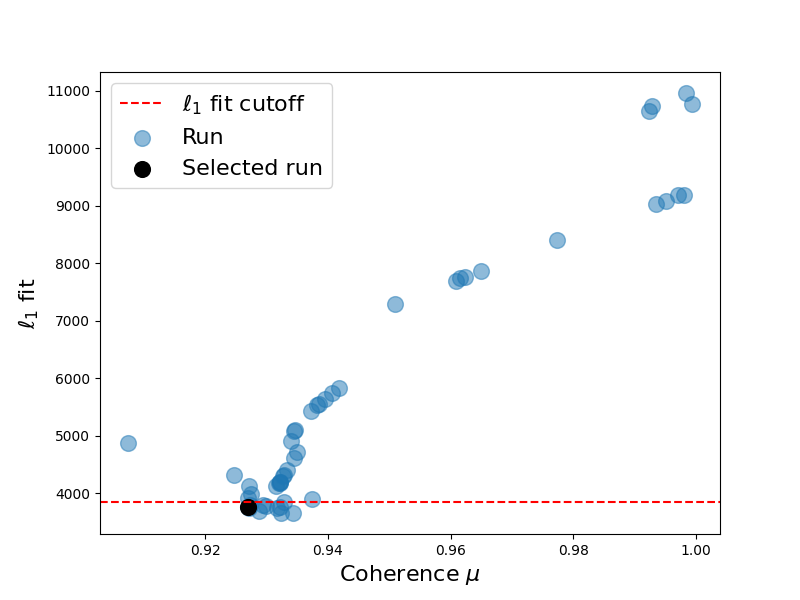
\includegraphics[width=0.33\textwidth]{fichiers_latex/Chap2/figs/fit_Samson.png}}
  \hfil
  \subfloat[Jasper Ridge]{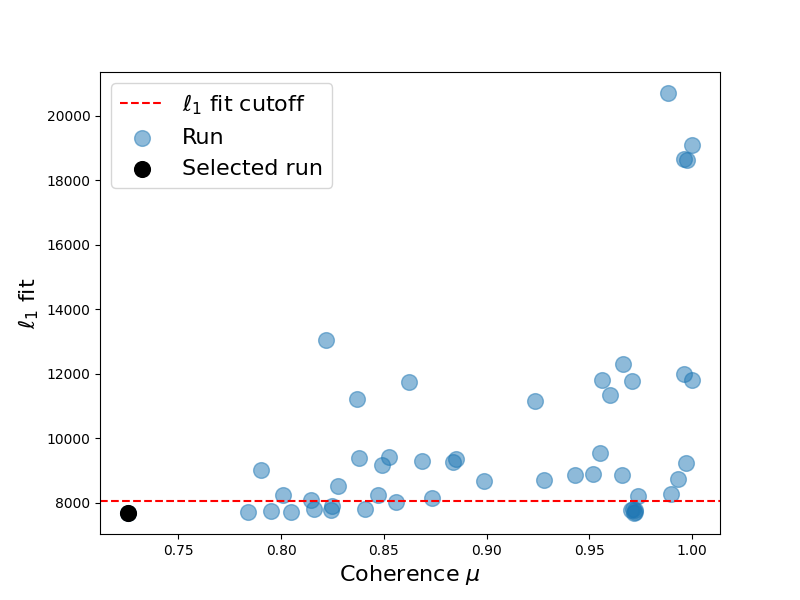
\includegraphics[width=0.33\textwidth]{fichiers_latex/Chap2/figs/fit_JR.png}}
  \hfil
  \subfloat[Urban4]{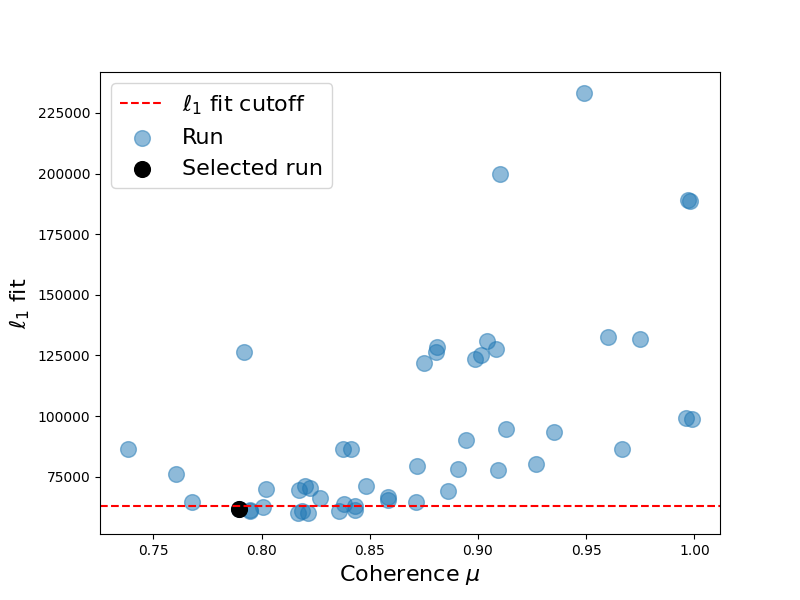
\includegraphics[width=0.33\textwidth]{fichiers_latex/Chap2/figs/fit_U4.png}}
  \hfil
  \subfloat[Urban6]{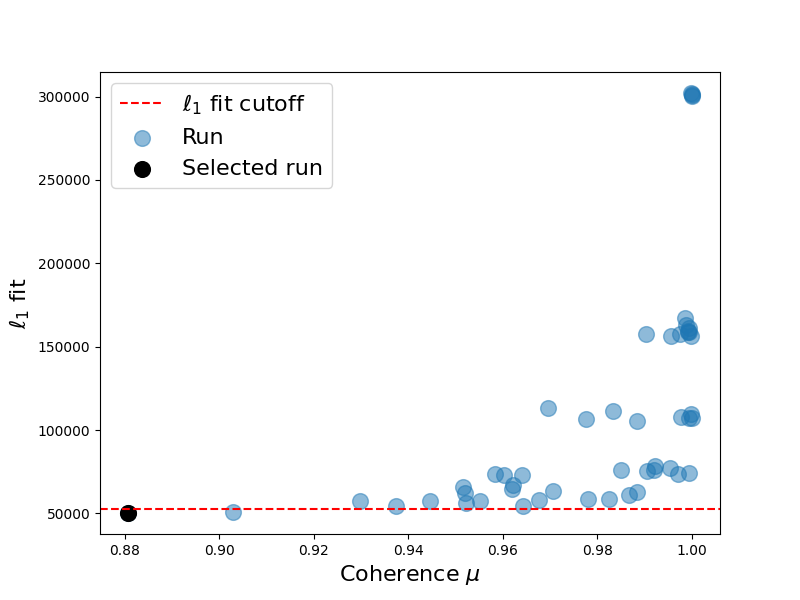
\includegraphics[width=0.33\textwidth]{fichiers_latex/Chap2/figs/fit_U6.png}}
  \hfil
  \subfloat[APEX]{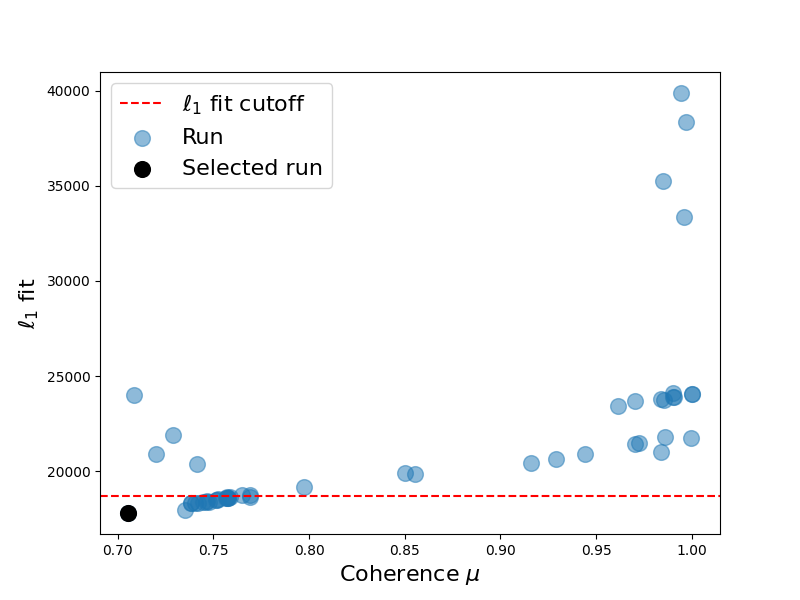
\includegraphics[width=0.33\textwidth]{fichiers_latex/Chap2/figs/fit_APEX.png}}
  \hfil
  \subfloat[WDC]{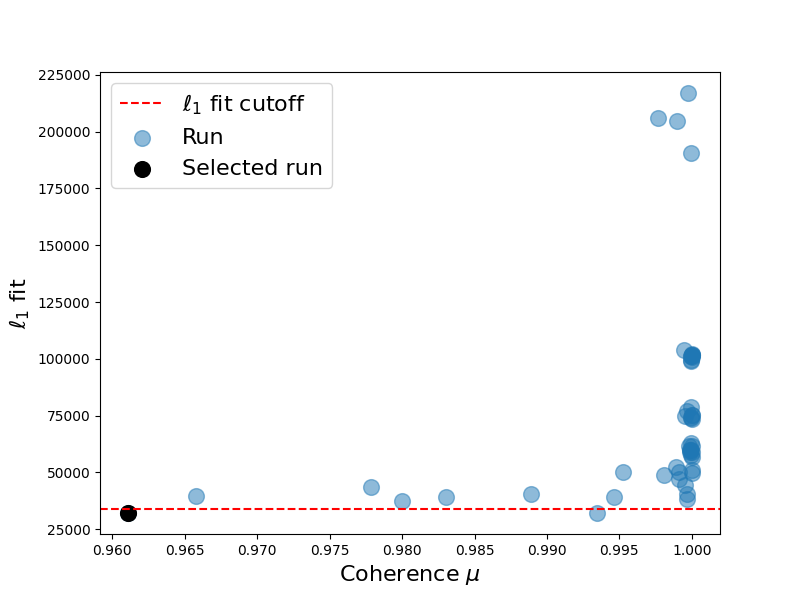
\includegraphics[width=0.33\textwidth]{fichiers_latex/Chap2/figs/fit_WDC.png}}
  \caption{\revision{Illustration of the model selection procedure on six datasets
    using $M=50$ runs. Runs are illustrated by blue dots and the
    selected one is in black. The selected run is the one with lowest coherence
    $\mu$ under the dashed red line representing the $\ell_1$ fit threshold, see Alg.~\ref{alg:criterion}.}}
  \label{fig:MSP}
\end{figure*}


\begin{algorithm}[h]
  \caption{Model Selection Procedure}\label{alg:criterion}
  \begin{algorithmic}[1]
    \State \textbf{Input:} $M$ (number of runs); $\ell_2$-normalized data $\Y$ in $\Real^{p \times n}$; $r$ (number of
    endmembers); $T$ (number of outer iterations); $K_1$ (number of inner
    iterations for $\hat{\A}$); $K_2$ (number of inner iterations for $\hat{\B}$).
    \For{$m = 1, \ldots, M$} 
       \State Set random seed $s_m$.
       \State $\hat{\E}_m, \hat{\A}_m \gets \text{EDAA}(\Y, r, T, K_1, K_2, s_m)$ 
       \Comment{See (\ref{alg:EDAA})}
       \State $\text{fit}_m \gets ||\Y - \hat{\E}_m \hat{\A}_m||_1$
       % \State Compute maximal pairwise spectral correlation $\mu_m$ on $\hat{\E}_m$.
       \State Compute coherence $\mu_m$ on $\hat{\E}_m$.
       \Comment{See (\ref{eq:coherence})}
    \EndFor
    \State $\text{fit}_{\min} \gets \min \{ \text{fit}_1, \ldots, \text{fit}_M \}$
    \State $\mathcal{I} \gets \{m \; | \; \text{fit}_m \leq 1.05 \times \text{fit}_{\min} \}$
    \Comment{Subset of models.}
    \State $\text{best} \gets \arg \min \{\mu_i, i \in \mathcal{I}\}$
    \State \textbf{Return:} $\hat{\E}_{\text{best}}$, $\hat{\A}_{\text{best}}$.
  \end{algorithmic}
\end{algorithm}

\section{Experiments}
\label{sec:EDAA_exp}

\revision{We have performed experiments on one simulated dataset with different noise and purity levels as well as six standard real datasets whose descriptions are given below.}

\subsection{Data description}

\begin{enumerate}

\item Simulated dataset:
\revision{For our study, we chose six endmembers from the USGS library and generated a 1000-pixel data cube using the methodology outlined in~\cite{ambikapathi_chance-constrained_2011}. This approach allowed us to vary the purity level of the pixels by adjusting the parameter $\rho$, which is used in Table \ref{table:sim}. Specifically, lower values of $\rho$ correspond to pixels that are less pure, while higher values indicate greater purity. By manipulating this parameter, we were able to simulate a range of real-world scenarios and evaluate the robustness of our algorithm under different conditions.}

\item Samson: 
  The Samson\footnote{downloaded at \href{https://rslab.ut.ac.ir/data}{https://rslab.ut.ac.ir/data}} hyperspectral
image is a 95x95 pixels sub-region of a larger image captured using 156 bands spanning from 401 to 889 nm.
Three main materials have been identified: Tree, Soil and Water.
Note that we use a different ground truth from \cite{rasti_misicnet_2022} that we selected for its sharper details on the abundances.

\item Jasper Ridge:
\addtocounter{footnote}{-1}
The Jasper Ridge\footnotemark~hyperspectral
image is a 100x100 pixels sub-region of a larger image initially captured
using 224 bands spanning from 380 to 2500 nm.
In total, 198 bands remain as 26 were removed as a pre-processing step due to
dense water vapor and atmospheric effects.
Four main materials have been identified: Tree, Dirt, Water and Road.

\item Urban4 and Urban6:
\addtocounter{footnote}{-1}
The Urban\footnotemark~hyperspectral image is a 307x307 pixels image collected by the
Hyperspectral Digital Image Collection Experiment (HYDICE) \cite{rickard_hydice_1993} sensor using
210 bands spanning from 400 to 2500 nm.
In total, 162 bands remain as 48 were removed as a pre-processing step due to
dense water vapor and atmospheric effects.
There exists three versions of this dataset w.r.t. the number of endmembers.
In this study, we focus on the two extremes: Urban4 contains 4 endmembers
(Asphalt Road, Grass, Tree and Roof) and
Urban6 contains two additional materials: Dirt and Metal, making it more challenging.

\item APEX:
The APEX \cite{schaepman_advanced_2015} hyperspectral image that we consider in
this paper is a 111x122 pixels cropped region\footnote{downloaded at \href{https://github.com/BehnoodRasti/MiSiCNet}{https://github.com/BehnoodRasti/MiSiCNet}} of a larger image captured over
285 bands spanning from 413 to 2420nm.
Four main materials were identified: Road, Tree, Roof and Water.
\rev{Note that the ground truth abundance map for water appears to contain shadows due to the sunlight direction (see figure~\ref{fig:APEX}). This is a common issue when dealing with real remote sensing data and we cannot expect the semi-automated ground truth abundances map generation to be perfect.}


\item Washington DC Mall:
\addtocounter{footnote}{-1}
The Washington DC Mall (WDC) hyperspectral dataset\footnotemark~consists in a
319x292 pixels image captured by the HYDICE \cite{rickard_hydice_1993} sensor
over 191 bands spanning from 400 to 2400 nm.
Six main materials were identified: Grass, Tree, Roof, Road, Water and Trail.

\end{enumerate}

According to \cite{zhu_hyperspectral_2017} (Samson, Jasper Ridge and Urban) and
\cite{rasti_misicnet_2022} (APEX and WDC), the endmembers
spectra were manually selected from the images and the ground truth abundances
were set by the fully constrained least squares (FCLS) unmixing algorithm.
Illustrations of the datasets and their ground truth endmembers are available in
the supplementary material.

\subsection{Experimental setup}

\rev{
We compare our approach to nine competitive methods from different unmixing
categories:}

\begin{itemize}

  \item \rev{Geometrical unmixing baseline: FCLS \cite{heinz_fully_2001} using VCA
    \cite{nascimento_vertex_2005} to extract endmembers.
    Our implementation of the FCLS algorithm uses the \emph{DecompSimplex}
    routine implemented in SPAMS\footnote{\href{http://thoth.inrialpes.fr/people/mairal/spams/}{http://thoth.inrialpes.fr/people/mairal/spams/}}.
    This method relies on the active-set algorithm \cite{nocedal_numerical_1999}
    that enables significantly faster convergence than generic quadratic
    programming solvers by leveraging the underlying sparsity of the abundances
    as noted by \cite{chen_fast_2014}.}

  \item \rev{Deep learning unmixing: Endnet\footnote{implementation at \href{https://github.com/burknipalsson/hu\_autoencoders}{https://github.com/burknipalsson/hu\_autoencoders}}
    \cite{ozkan_endnet_2018} using VCA \cite{nascimento_vertex_2005} to
    initialize the endmembers, MiSiCNet\footnote{implementation at
      \href{https://github.com/BehnoodRasti/MiSiCNet}{https://github.com/BehnoodRasti/MiSiCNet}}
    \cite{rasti_misicnet_2022} and the deep unrolling network ADMMNet\footnote{no implementation available online} \cite{zhou_admm-based_2021}.}

  \item \rev{NMF-based blind unmixing: minimum-volume-constraint non-negative matrix factorization (MVCNMF)\footnote{implementation found \href{https://www.dropbox.com/s/6pk77pgsz48o303/NCAA\_v1.zip?dl=0}{here}}~\cite{miao_endmember_2007}, non-negative matrix factorization quadratic
    minimum volume (NMF-QMV)\footnote{implementation at
      \href{https://github.com/LinaZhuang/NMF-QMV\_demo}{https://github.com/LinaZhuang/NMF-QMV\_demo}}
    \cite{zhuang_regularization_2019} using the \emph{boundary} term as the
    quadratic minimum volume penalty, near-convex archetypal analysis (NCAA)\footnote{implementation found \href{https://www.dropbox.com/s/6pk77pgsz48o303/NCAA\_v1.zip?dl=0}{here}}~\cite{de_handschutter_near-convex_2019} and AA \cite{cutler_archetypal_1994} using
    the implementation from~\cite{chen_fast_2014} developed in SPAMS.}

    \revision{The approach denoted as AA involves solving~(\ref{eq:AA2}) using an active-set method to optimize the convex sub-problems. This method is a conventional alternating approach that uses a fixed initialization ($\A$ and $\B$ entries are set to 0) and a fixed number of iterations ($T=100$). While AA is a well-known method, it has not been thoroughly evaluated on various real-world unmixing datasets. Therefore, we include it as a competing method in our study to compare its performance with other state-of-the-art algorithms. By using AA, we can also assess the improvements in optimization achieved by EDAA since the underlying model (\ref{eq:AA2}) is the same for both methods. This comparison enables us to gain insights into the benefits of EDAA for hyperspectral unmixing.}  

    \item \rev{Finally, we include a recent technique addressing spectral variability: SeCoDe\footnote{implementation at \href{https://github.com/danfenghong/IEEE\_TGRS\_SeCoDe}{https://github.com/danfenghong/IEEE\_TGRS\_SeCoDe}}~\cite{yao_sparsity-enhanced_2021}.}
\end{itemize}

  
To quantitatively evaluate the performance of the selected methods, we consider two metrics that are computed both globally and individually for each endmember.
On one hand, we measure the quality of the generated abundances by means of the
abundances root mean square error (RMSE) in percent between the ground truth and the
estimated abundances:

\begin{equation} \label{eq:RMSE}
  \text{RMSE}(\A, \hat{\A}) = 100 \times \sqrt{\frac{1}{r n} \sum_{i=1}^r \sum_{j=1}^n \left( \A_{i, j} - \hat{\A}_{i, j} \right)^2}.
\end{equation}

On the other hand, we assess the quality of the estimated endmembers spectra by
using the spectral angle distance (SAD) in degrees between the ground truth and
the generated endmembers:

\begin{equation}  \label{eq:SAD}
  \text{SAD}(\E, \hat{\E}) = \frac{180}{\pi} \times \frac{1}{r} \sum_{i=1}^r \arccos \left( \frac{\langle \ee_i, \hat{\ee}_i \rangle}{||\ee_i||_2 ||\hat{\ee}_i||_2} \right),
\end{equation}

where $\ee_i$ denotes the
$i$-th column of $\E$, \ie the spectrum of the $i$-th endmember.

\subsection{Unmixing experiments}

\begin{table}[h]
  \centering
  \captionof{table}{\revision{Abundances RMSE and endmembers SAD for the simulated dataset with different noise and purity levels. The best results are shown in bold. The second best results are underlined.}}
  % \begin{adjustbox}{width=\textwidth}
    \resizebox{\textwidth}{!}{
\begin{tabular}{c|c|ccc|ccc}
\toprule
\multirow{3}{*}{Methods} & \multirow{3}{*}{$\rho$} & \multicolumn{3}{c|}{RMSE}                                                   & \multicolumn{3}{c}{SAD}                               \\ \cline{3-8} 
                         &                      & \multicolumn{3}{c|}{SNR (dB)}                                               & \multicolumn{3}{c}{SNR (dB)}                          \\ \cline{3-8} 
                         &                      & \multicolumn{1}{c|}{20} & \multicolumn{1}{c|}{30} & \multicolumn{1}{c|}{40} & \multicolumn{1}{c|}{20} & \multicolumn{1}{c|}{30} & 40 \\ \hline
\multirow{3}{*}{FCLS \cite{heinz_fully_2001}}   
      & 0.7     &  16.53   &   17.15   &   17.97   &   7.20    &   7.18    & 7.38  \\
     & 0.85     &  12.96   &   11.44   &  10.15    &   3.86    &  3.05     &  2.45  \\
      & 1.0     &  8.03   &  4.43    &  3.31    &   1.84    &   0.58    &  \textbf{0.17}  \\ 
\hline
%\multirow{3}{*}{MiSiCNet \cite{rasti_misicnet_2022}}   
%      & 0.7      &  28.01   &  27.78    &   26.91   &   14.35    &   14.43    &  14.45 \\
%      & 0.85     &   15.35  &  15.58    &   15.63   &   12.92    &    12.95   &  12.97  \\
%      & 1.0      &  3.04   &   3.03   &  3.04    &   11.99    &   12.07    &   12.08 \\ 
%\hline
\multirow{3}{*}{MiSiCNet \cite{rasti_misicnet_2022} ($\lambda=0.1$)}   
      & 0.7      &  \underline{10.60}   &  \underline{8.64}   &   \underline{8.31}   &   \textbf{3.94}   &   \textbf{1.88}   &  \textbf{1.58} \\
      & 0.85     &   13.76  &   8.62  &   \underline{7.68}   &   4.70   &  1.20    &  \textbf{0.75}  \\
      & 1.0      &   15.08  &  6.42   &  3.73    &   5.11   &   1.12   &  0.39  \\ 
\hline
\multirow{3}{*}{\rev{ADMMNet} \cite{zhou_admm-based_2021}}   
      & 0.7      &   15.49  &  16.92    &  16.68   &   11.44    &  13.76   &  13.48 \\
      & 0.85     &  17.18   &   19.54   &  19.58   &   8.52    &  10.23   &  9.93 \\
      & 1.0      &   21.13  &  16.57    &  16.60   &   9.03    &   6.26  &  6.55 \\
\hline
\multirow{3}{*}{\rev{MVCNMF} \cite{miao_endmember_2007}}   
      & 0.7      &   15.80  &   9.75   &  15.53   &    6.85   &  2.52   &  6.85 \\
      & 0.85     &  9.88   &   9.80   &  9.54   &    \textbf{1.85}   &  \textbf{1.16}   &  \underline{0.76} \\
      & 1.0      &   6.84  &   7.03   &   3.55  &   1.12    &  0.78   &  \textbf{0.17} \\
\hline
\multirow{3}{*}{NMFQMV \cite{zhuang_regularization_2019}}   
      & 0.7      &  \textbf{10.11}   &   \textbf{8.32}   &   \textbf{7.36}   &   \underline{4.96}    &   \underline{4.76}    &  \underline{3.32} \\
      & 0.85     &  10.58   &   \textbf{7.11}   &  \textbf{6.79}    &   2.91    &   \underline{1.18}    &  0.98  \\
      & 1.0      &   11.24  &   6.62   &   3.80   &   3.25    &  1.54     &  0.41  \\
\hline

\multirow{3}{*}{\rev{SeCoDe} \cite{yao_sparsity-enhanced_2021}}   
           & 0.7      &  13.49   &   13.36   &  13.62   &   16.06    &  16.38   &  16.54 \\
      & 0.85     &  13.56   &   14.76   &  14.69   &  14.62     &   15.79  & 15.73  \\
      & 1.0      &   7.88  &   4.74   &  4.35   &    7.76   &   5.07  &  4.76 \\
\hline
\multirow{3}{*}{\rev{NCAA} \cite{de_handschutter_near-convex_2019}}   
           & 0.7      &   14.62  &   13.43   &   14.64  &   8.32    &   8.00  &  7.44 \\
      & 0.85     &  12.15   &   7.66   &  7.19   &   5.72    &  2.56   &  1.10 \\
      & 1.0      &   11.61  &   \underline{3.20}   &  3.25   &    5.37   &  1.70   &  0.71 \\
\hline


\multirow{3}{*}{AA ($T=100$)}   
      & 0.7      &  17.67   &   17.23   &  17.18    &   7.61    &   6.71    &  6.43 \\
      & 0.85     &   \underline{9.44}  &  \underline{8.23}    &   8.04   &   \underline{2.55}    &   2.09    &  1.86  \\
      & 1.0      &   \textbf{5.13}  &   \textbf{2.98}   &   \textbf{2.75}   &   \textbf{0.88}    &   \textbf{0.45}    &  0.34  \\ 
\hline
%\multirow{3}{*}{EDAA}   
%      & 0.7      &   15.87  &   15.93   &   15.66   &   7.73    &    6.87   &  6.85 \\
%      & 0.85     &  13.03   &   11.59   &   11.48   &   2.96    &   2.32    &  2.23  \\
%      & 1.0      &   8.67  &   6.79   &   6.55   &   1.07    &   0.53    &  0.39  \\ 
%\hline
%\multirow{3}{*}{EDAA ($K_1=K_2=20$)}   
%      & 0.7      &   15.76   &  14.33   &   15.04   &   6.27   &   5.62   &  5.78 \\
%      & 0.85     &  9.94   &  8.99   &  8.70    &   2.74   &   2.33   &  1.97  \\
%      & 1.0      &  7.38   &  3.74   &   3.23   &   1.07   &  0.54    &  0.34  \\
%\hline
\multirow{3}{*}{EDAA ($K_1=K_2=30$)}   
      & 0.7      &   14.35   &  13.75   &   14.91   &   5.50   &   5.01   &  6.52 \\
      & 0.85     &  \textbf{8.84}   &  8.37   &  8.37    &   2.63   &   2.18   &  1.92  \\
      & 1.0      &  \underline{5.82}   &  4.26   &   \underline{2.89}   &   \underline{0.96}   &  \underline{0.51}    &  0.33  \\
\bottomrule
\end{tabular}
}
  % \end{adjustbox}
  \label{table:sim}
\end{table}

\revision{
Table~\ref{table:sim} presents the results of our unmixing accuracy evaluation on the simulated dataset. Our analysis indicates that the performance of the AA variants (active-set based and EDAA) is lower in scenarios where the pixels are highly mixed ($\rho=0.7$) when compared to geometrically motivated methods, such as MiSiCNet, MVCNMF and NMF-QMV, which do not rely directly on the pixel values to estimate the endmembers. However, it is worth noting that the EDAA method performs better than the plain AA method in this setting, thanks to its advanced model selection. In the case where pure pixels are present ($\rho=1.0$), the AA model formulation~(\ref{eq:AA2}) yields the best results, as it estimates the endmembers as convex combinations of the pixels. This approach is more robust to noise than the FCLS method. For the medium case ($\rho=0.85$), both AA and EDAA exhibit better performance than MiSiCNet and NMF-QMV for low Signal-to-Noise Ratio (SNR) due to their greater robustness to noise. However, they are outperformed by MiSiCNet and NMF-QMV for high SNR, as there are no pure pixels available for these methods to leverage.
}

\begin{table}[h]
  \centering
  \captionof{table}{Abundances RMSE on six real datasets. The best results are
    shown in bold. The second best results are underlined.}
  % \begin{adjustbox}{width=\textwidth}
    % \begin{tabular}{c | c | c c c c c c c}
%   \toprule
%   & & FCLSU & NMF-QMV & AA & RAA & CNNAEU & MiSiCNet & EDAA \\
%   \hline
%   \multirow{4}{*}{Samson}
%   & Soil & 11.28 & 13.67 & 6.16 & 6.02 & 25.82 & 18.18 & \textbf{5.91} \\
%   & Tree & 9.13 & 8.4 & 4.00 & 4.12 & 22.88 & 17.91 & \textbf{3.84} \\
%   & Water & 5.05 & 11.61 & 2.30 & \textbf{2.08} & 25.32 & 31.30 & 2.73\\
%   \cline{2-9}
%   & Overall & 8.88 & 11.44 & 4.44 & 4.38 & 25.18 & 23.32 & \textbf{4.36}\\
%   \hline
%   \hline
%   \multirow{5}{*}{Jasper Ridge}
%   & Dirt & 21.23 & 19.97 & 10.24 & 10.54 & 38.42 & 22.11 & \textbf{8.10} \\
%   & Road & 24.72 & 26.13 & 9.79 & 8.75 & 31.22 & 24.89 & \textbf{7.84} \\
%   & Tree & 11.20 & 14.55 & \textbf{6.32} & 9.87 & 27.82 & 9.57 & 7.76 \\
%   & Water & 13.61 & 19.81 & 6.77 & \textbf{5.00} & 21.28 & 11.44 & 5.66 \\
%   \cline{2-9}
%   & Overall & 18.52 & 20.53 & 8.46 & 8.81 & 30.75 & 18.24 & \textbf{7.41} \\
%   \hline
%   \hline
%   \multirow{5}{*}{Urban4}
%   & Road & 30.54 & 20.25 & 11.12 & \textbf{8.80} & 26.74 & 37.69 & 13.00 \\
%   & Grass & 32.99 & 20.22 & 11.55 & 11.29 & 30.53 & 31.64 & \textbf{9.55} \\
%   & Roof & 15.40 & 13.29 & 7.28 & \textbf{5.31} & 20.24 & 15.63 & 8.21 \\
%   & Tree & 20.02 & 21.56 & 8.62 & 8.41 & 21.33 & 24.52 & \textbf{6.96} \\
%   \cline{2-9}
%   & Overall & 25.78 & 19.11 & 9.80 & \textbf{8.71} & 25.22 & 28.58 & 9.70\\
%   \hline
%   \hline
%   \multirow{7}{*}{Urban6}
%   & Road & 31.61 & 24.81 & 19.23 & 19.97 & 27.86 & 19.32 & \textbf{13.63} \\
%   & Grass & 23.62 & 27.97 & \textbf{9.73} & 27.02 & 36.36 & 25.67 & 10.05 \\
%   & Roof & 13.00 & 16.39 & 10.92 & \textbf{5.89} & 13.36 & 13.76 & 9.22 \\
%   & Tree & 16.14 & 19.95 & 14.45 & 20.07 & 22.41 & 24.53 &\textbf{8.79} \\
%   & Dirt & 25.06 & 24.31 & 27.76 & 24.82 & 29.27 & 15.58 & \textbf{9.70} \\
%   & Metal & \textbf{12.99} & 13.40 & 17.53 & 19.22 & 26.11 & 33.67 & 19.25 \\
%   \cline{2-9}
%   & Overall & 21.54 & 21.74 & 17.66 & 20.62 & 27.25 & 23.09 & \textbf{12.34} \\
%   \hline
%   \hline
%   \multirow{5}{*}{APEX}
%   & Road & 33.31 & 31.43 & 34.12 & 35.68 & 35.34 & 13.67 & \textbf{13.12} \\
%   & Tree & 20.97 & 24.62 & 22.49 & 24.61 & 14.29 & 14.92 & \textbf{14.13} \\
%   & Roof & 14.15 & 14.73 & 18.54 & 19.81 & 28.29 & \textbf{11.38} & 11.79 \\
%   & Water & 18.03 & 17.99 & 16.90 & \textbf{16.85} & 35.40 & 19.84 & 16.95 \\
%   \cline{2-9}
%   & Overall & 22.77 & 23.10 & 23.98 & 25.27 & 24.10 & 15.27 & \textbf{14.13} \\
%   \hline
%   \hline
%   \multirow{7}{*}{WDC}
%   & Grass & 30.90 & 34.69 & 31.92 & 31.03 & 43.05 & \textbf{24.51} & 31.75 \\
%   & Tree & 22.42 & 19.90 & 20.13 & 15.96 & 35.03 & \textbf{10.55} & 11.08 \\
%   & Road & 27.90 & 22.49 & 38.87 & 35.42 & 28.57 & 18.16 & \textbf{9.48} \\
%   & Roof & \textbf{8.71} & 19.81 & 20.89 & 20.45 & 23.92 & 18.88 & 33.99 \\
%   & Water & 17.76 & 20.34 & 14.06 & 14.00 & 36.17 & 18.02 & \textbf{9.96} \\
%   & Trail & 12.80 & 12.36 & 15.24 & 15.92 & 28.40 & 9.66 & \textbf{7.29} \\
%   \cline{2-9}
%   & Overall & 21.57 & 22.60 & 25.17 & 23.59 & 33.59 & \textbf{17.40} & 20.53\\
%   \bottomrule
% \end{tabular}

% \begin{tabular}{c | c | c c c c c c c}
%   \toprule
%   & & FCLSU & CNNAEU & MiSiCNet & NMF-QMV & AA & RAA & EDAA \\
%   \hline
%   \multirow{4}{*}{Samson}
%   & Soil & 11.28 & 25.82 & 18.18 & 13.67 & 6.16 & 6.02 & \textbf{5.91} \\
%   & Tree & 9.13 & 22.88 & 17.91 & 8.4 & 4.00 & 4.12 & \textbf{3.84} \\
%   & Water & 5.05 & 25.32 & 31.30 & 11.61 & 2.30 & \textbf{2.08} & 2.73\\
%   \cline{2-9}
%   & Overall & 8.88 & 25.18 & 23.32 & 11.44 & 4.44 & 4.38 & \textbf{4.36}\\
%   \hline
%   \hline
%   \multirow{5}{*}{Jasper Ridge}
%   & Dirt & 21.23 & 38.42 & 22.11 & 19.97 & 10.24 & 10.54 & \textbf{8.10} \\
%   & Road & 24.72 & 31.22 & 24.89 & 26.13 & 9.79 & 8.75 & \textbf{7.84} \\
%   & Tree & 11.20 & 27.82 & 9.57 & 14.55 & \textbf{6.32} & 9.87 & 7.76 \\
%   & Water & 13.61 & 21.28 & 11.44 & 19.81 & 6.77 & \textbf{5.00} & 5.66 \\
%   \cline{2-9}
%   & Overall & 18.52 & 30.75 & 18.24 & 20.53 & 8.46 & 8.81 & \textbf{7.41} \\
%   \hline
%   \hline
%   \multirow{5}{*}{Urban4}
%   & Road & 30.54 & 26.74 & 37.69 & 20.25 & 11.12 & \textbf{8.80} & 13.00 \\
%   & Grass & 32.99 & 30.53 & 31.64 & 20.22 & 11.55 & 11.29 & \textbf{9.55} \\
%   & Roof & 15.40 & 20.24 & 15.63 & 13.29 & 7.28 & \textbf{5.31} & 8.21 \\
%   & Tree & 20.02 & 21.33 & 24.52 & 21.56 & 8.62 & 8.41 & \textbf{6.96} \\
%   \cline{2-9}
%   & Overall & 25.78 & 25.22 & 28.58 & 19.11 & 9.80 & \textbf{8.71} & 9.70\\
%   \hline
%   \hline
%   \multirow{7}{*}{Urban6}
%   & Road & 31.61 & 27.86 & 19.32 & 24.81 & 19.23 & 19.97 & \textbf{13.63} \\
%   & Grass & 23.62 & 36.36 & 25.67 & 27.97 & \textbf{9.73} & 27.02 & 10.05 \\
%   & Roof & 13.00 & 13.36 & 13.76 & 16.39 & 10.92 & \textbf{5.89} & 9.22 \\
%   & Tree & 16.14 & 22.41 & 24.53 & 19.95 & 14.45 & 20.07 &\textbf{8.79} \\
%   & Dirt & 25.06 & 29.27 & 15.58 & 24.31 & 27.76 & 24.82 & \textbf{9.70} \\
%   & Metal & \textbf{12.99} & 26.11 & 33.67 & 13.40 & 17.53 & 19.22 & 19.25 \\
%   \cline{2-9}
%   & Overall & 21.54 & 27.25 & 23.09 & 21.74 & 17.66 & 20.62 & \textbf{12.34} \\
%   \hline
%   \hline
%   \multirow{5}{*}{APEX}
%   & Road & 33.31 & 35.34 & 13.67 & 31.43 & 34.12 & 35.68 & \textbf{13.12} \\
%   & Tree & 20.97 & 14.29 & 14.92 & 24.62 & 22.49 & 24.61 & \textbf{14.13} \\
%   & Roof & 14.15 & 28.29 & \textbf{11.38} & 14.73 & 18.54 & 19.81 & 11.79 \\
%   & Water & 18.03 & 35.40 & 19.84 & 17.99 & 16.90 & \textbf{16.85} & 16.95 \\
%   \cline{2-9}
%   & Overall & 22.77 & 24.10 & 15.27 & 23.10 & 23.98 & 25.27 & \textbf{14.13} \\
%   \hline
%   \hline
%   \multirow{7}{*}{WDC}
%   & Grass & 30.90 & 43.05 & \textbf{24.51} & 34.69 & 31.92 & 31.03 & 31.75 \\
%   & Tree & 22.42 & 35.03 & \textbf{10.55} & 19.90 & 20.13 & 15.96 & 11.08 \\
%   & Road & 27.90 & 28.57 & 18.16 & 22.49 & 38.87 & 35.42 & \textbf{9.48} \\
%   & Roof & \textbf{8.71} & 23.92 & 18.88 & 19.81 & 20.89 & 20.45 & 33.99 \\
%   & Water & 17.76 & 36.17 & 18.02 & 20.34 & 14.06 & 14.00 & \textbf{9.96} \\
%   & Trail & 12.80 & 28.40 & 9.66 & 12.36 & 15.24 & 15.92 & \textbf{7.29} \\
%   \cline{2-9}
%   & Overall & 21.57 & 33.59 & \textbf{17.40} & 22.60 & 25.17 & 23.59 & 20.53\\
%   \bottomrule
% \end{tabular}
% \begin{tabular}{c | c | c c c c c c c}
%   \toprule
%   & & FCLSU \cite{nascimento_vertex_2005, heinz_fully_2001} & CNNAEU \cite{palsson_convolutional_2021} & MiSiCNet \cite{rasti_misicnet_2022} & NMF-QMV \cite{zhuang_regularization_2019} & AA & RAA & EDAA \\
%   \hline
%   \multirow{4}{*}{Samson}
%   & Soil & 11.28 & 45.23 & 6.47 & 13.67 & 6.16 & \underline{6.02} & \textbf{5.91} \\
%   & Tree & 9.13 & 45.83 & 5.38 & 8.4 & \underline{4.00} & 4.12 & \textbf{3.84} \\
%   & Water & 5.05 & 18.78 & 3.47 & 11.61 & \underline{2.30} & \textbf{2.08} & 2.73\\
%   \cline{2-9}
%   & Overall & 8.88 & 39.02 & 5.25 & 11.44 & 4.44 & \underline{4.38} & \textbf{4.36}\\
%   \hline
%   \hline
%   \multirow{5}{*}{Jasper Ridge}
%   & Dirt & 21.23 & 38.17 & 21.68 & 19.97 & \underline{10.24} & 10.54 & \textbf{8.10} \\
%   & Road & 24.72 & 43.87 & 24.94 & 26.13 & 9.79 & \underline{8.75} & \textbf{7.84} \\
%   & Tree & 11.20 & 32.93 & \textbf{3.41} & 14.55 & \underline{6.32} & 9.87 & 7.76 \\
%   & Water & 13.61 & 28.28 & 7.07 & 19.81 & 6.77 & \textbf{5.00} & \underline{5.66} \\
%   \cline{2-9}
%   & Overall & 18.52 & 37.83 & 16.98 & 20.53 & \underline{8.46} & 8.81 & \textbf{7.41} \\
%   \hline
%   \hline
%   \multirow{5}{*}{Urban4}
%   & Road & 30.54 & 38.22 & \underline{10.30} & 20.25 & 11.12 & \textbf{8.80} & 13.00 \\
%   & Grass & 32.99 & 49.72 & 12.35 & 20.22 & 11.55 & \underline{11.29} & \textbf{9.55} \\
%   & Roof & 15.40 & 25.15 & 8.01 & 13.29 & \underline{7.28} & \textbf{5.31} & 8.21 \\
%   & Tree & 20.02 & 41.04 & 8.78 & 21.56 & 8.62 & \underline{8.41} & \textbf{6.96} \\
%   \cline{2-9}
%   & Overall & 25.78 & 40.14 & 10.00 & 19.11 & 9.80 & \textbf{8.71} & \underline{9.70}\\
%   \hline
%   \hline
%   \multirow{7}{*}{Urban6}
%   & Road & 31.61 & 31.43 & \underline{19.18} & 24.81 & 19.23 & 19.97 & \textbf{13.63} \\
%   & Grass & 23.62 & 49.55 & 18.84 & 27.97 & \textbf{9.73} & 27.02 & \underline{10.05} \\
%   & Roof & 13.00 & 21.81 & \underline{7.41} & 16.39 & 10.92 & \textbf{5.89} & 9.22 \\
%   & Tree & 16.14 & 34.99 & \underline{11.72} & 19.95 & 14.45 & 20.07 &\textbf{8.79} \\
%   & Dirt & 25.06 & 59.12 & \underline{23.95} & 24.31 & 27.76 & 24.82 & \textbf{9.70} \\
%   & Metal & \textbf{12.99} & 26.85 & 33.67 & \underline{13.40} & 17.53 & 19.22 & 19.25 \\
%   \cline{2-9}
%   & Overall & 21.54 & 41.17 & \underline{16.27} & 21.74 & 17.66 & 20.62 & \textbf{12.34} \\
%   \hline
%   \hline
%   \multirow{5}{*}{APEX}
%   & Road & 33.31 & 36.42 & 32.66 & \underline{31.43} & 34.12 & 35.68 & \textbf{13.12} \\
%   & Tree & 20.97 & 39.99 & \underline{19.97} & 24.62 & 22.49 & 24.61 & \textbf{14.13} \\
%   & Roof & \underline{14.15} & 32.69 & 18.42 & 14.73 & 18.54 & 19.81 & \textbf{11.79} \\
%   & Water & 18.03 & 32.32 & \underline{16.88} & 17.99 & 16.90 & \textbf{16.85} & 16.95 \\
%   \cline{2-9}
%   & Overall & \underline{22.77} & 35.76 & 22.86 & 23.10 & 23.98 & 25.27 & \textbf{14.13} \\
%   \hline
%   \hline
%   \multirow{7}{*}{WDC}
%   & Grass & \textbf{30.90} & 46.77 & 31.61 & 34.69 & 31.92 & \underline{31.03} & 31.75 \\
%   & Tree & 22.42 & 36.06 & 23.64 & 19.90 & 20.13 & \underline{15.96} & \textbf{11.08} \\
%   & Road & 27.90 & 34.64 & 34.91 & \underline{22.49} & 38.87 & 35.42 & \textbf{9.48} \\
%   & Roof & \textbf{8.71} & 14.84 & \underline{11.98} & 19.81 & 20.89 & 20.45 & 33.99 \\
%   & Water & 17.76 & 40.24 & 14.72 & 20.34 & 14.06 & \underline{14.00} & \textbf{9.96} \\
%   & Trail & 12.80 & 23.17 & \underline{12.07} & 12.36 & 15.24 & 15.92 & \textbf{7.29} \\
%   \cline{2-9}
%   & Overall & \underline{21.57} & 35.64 & 23.39 & 22.60 & 25.17 & 23.59 & \textbf{20.53}\\
%   \bottomrule
% \end{tabular}

% \begin{tabular}{c | c | c c c c c c c}
%   \toprule
%   & & FCLSU \cite{nascimento_vertex_2005, heinz_fully_2001} & Endnet \cite{ozkan_endnet_2018} & MiSiCNet \cite{rasti_misicnet_2022} & NMF-QMV \cite{zhuang_regularization_2019} & AA & RAA & EDAA \\
%   \hline
%   \multirow{4}{*}{Samson}
%   & Soil & 11.28 & 11.61 & 6.47 & 13.67 & 6.16 & \underline{6.02} & \textbf{5.74} \\
%   & Tree & 9.13 & 7.72 & 5.38 & 8.4 & \underline{4.00} & 4.12 & \textbf{3.77} \\
%   & Water & 5.05 & 6.86 & 3.47 & 11.61 & \underline{2.30} & \textbf{2.08} & 2.59\\
%   \cline{2-9}
%   & Overall & 8.88 & 8.97 & 5.25 & 11.44 & 4.44 & \underline{4.38} & \textbf{4.24}\\
%   \hline
%   \hline
%   \multirow{5}{*}{Jasper Ridge}
%   & Dirt & 21.23 & 18.26 & 21.68 & 19.97 & \underline{10.24} & 10.54 & \textbf{7.32} \\
%   & Road & 24.72 & 29.40 & 24.94 & 26.13 & 9.79 & \underline{8.75} & \textbf{7.61} \\
%   & Tree & 11.20 & 4.00 & \textbf{3.41} & 14.55 & \underline{6.32} & 9.87 & 6.63 \\
%   & Water & 13.61 & 22.38 & 7.07 & 19.81 & 6.77 & \textbf{5.00} & \underline{5.69} \\
%   \cline{2-9}
%   & Overall & 18.52 & 20.70 & 16.98 & 20.53 & \underline{8.46} & 8.81 & \textbf{6.85} \\
%   \hline
%   \hline
%   \multirow{5}{*}{Urban4}
%   & Road & 30.54 & 12.04 & 10.30 & 20.25 & 11.12 & \underline{8.80} & \textbf{8.62} \\
%   & Grass & 32.99 & 17.94 & 12.35 & 20.22 & 11.55 & \underline{11.29} & \textbf{9.28} \\
%   & Roof & 15.40 & 11.28 & 8.01 & 13.29 & 7.28 & \textbf{5.31} & \underline{6.37} \\
%   & Tree & 20.02 & 11.69 & 8.78 & 21.56 & 8.62 & \underline{8.41} & \textbf{6.27} \\
%   \cline{2-9}
%   & Overall & 25.78 & 13.52 & 10.00 & 19.11 & 9.80 & \underline{8.71} & \textbf{7.75}\\
%   \hline
%   \hline
%   \multirow{7}{*}{Urban6}
%   & Road & 31.61 & \underline{17.44} & 19.18 & 24.81 & 19.23 & 19.97 & \textbf{11.39} \\
%   & Grass & 23.62 & 31.47 & 18.84 & 27.97 & \textbf{9.73} & 27.02 & \underline{18.61} \\
%   & Roof & 13.00 & 9.35 & 7.41 & 16.39 & 10.92 & \textbf{5.89} & \underline{6.01} \\
%   & Tree & 16.14 & 15.50 & \underline{11.72} & 19.95 & 14.45 & 20.07 &\textbf{9.85} \\
%   & Dirt & 25.06 & 30.67 & \underline{23.95} & 24.31 & 27.76 & 24.82 & \textbf{15.94} \\
%   & Metal & \textbf{12.99} & 25.21 & 33.67 & \underline{13.40} & 17.53 & 19.22 & 15.86 \\
%   \cline{2-9}
%   & Overall & 21.54 & 23.09 & \underline{16.27} & 21.74 & 17.66 & 20.62 & \textbf{13.63} \\
%   \hline
%   \hline
%   \multirow{5}{*}{APEX}
%   & Road & 33.31 & \underline{29.32} & 32.66 & 31.43 & 34.12 & 35.68 & \textbf{16.54} \\
%   & Tree & 20.97 & \underline{18.18} & 19.97 & 24.62 & 22.49 & 24.61 & \textbf{14.48} \\
%   & Roof & \underline{14.15} & 15.88 & 18.42 & 14.73 & 18.54 & 19.81 & \textbf{11.27} \\
%   & Water & 18.03 & 17.47 & 16.88 & 17.99 & 16.90 & \underline{16.85} & \textbf{16.83} \\
%   \cline{2-9}
%   & Overall & 22.77 & \underline{20.90} & 22.86 & 23.10 & 23.98 & 25.27 & \textbf{14.94} \\
%   \hline
%   \hline
%   \multirow{7}{*}{WDC}
%   & Grass & \underline{30.90} & \textbf{27.35} & 31.61 & 34.69 & 31.92 & 31.03 & 32.53 \\
%   & Tree & 22.42 & 35.98 & 23.64 & 19.90 & 20.13 & \underline{15.96} & \textbf{11.46} \\
%   & Road & 27.90 & 38.49 & 34.91 & \underline{22.49} & 38.87 & 35.42 & \textbf{13.97} \\
%   & Roof & \textbf{8.71} & 27.04 & \underline{11.98} & 19.81 & 20.89 & 20.45 & 29.31 \\
%   & Water & 17.76 & \underline{12.94} & 14.72 & 20.34 & 14.06 & 14.00 & \textbf{9.63} \\
%   & Trail & 12.80 & 12.63 & \textbf{12.07} & \underline{12.36} & 15.24 & 15.92 & 13.19 \\
%   \cline{2-9}
%   & Overall & \underline{21.57} & 27.64 & 23.39 & 22.60 & 25.17 & 23.59 & \textbf{20.46}\\
%   \bottomrule
% \end{tabular}

% Remove RAA

%\begin{tabular}{c | c | c c c c | c c}
%  \toprule
%  & & FCLSU \cite{nascimento_vertex_2005, heinz_fully_2001} & Endnet \cite{ozkan_endnet_2018} & MiSiCNet \cite{rasti_misicnet_2022} & NMF-QMV \cite{zhuang_regularization_2019} & AA & EDAA \\
%  \hline
%  \multirow{4}{*}{Samson}
%  & Soil & 11.28 & 11.61 & 6.47 & 13.67 & \underline{6.16} & \textbf{5.74} \\
%  & Tree & 9.13 & 7.72 & 5.38 & 8.4 & \underline{4.00} & \textbf{3.77} \\
%  & Water & 5.05 & 6.86 & 3.47 & 11.61 & \textbf{2.30} & \underline{2.59}\\
%  \cline{2-8}
%  & Overall & 8.88 & 8.97 & 5.25 & 11.44 & \underline{4.44} & \textbf{4.24}\\
%  \hline
%  \hline
%  \multirow{5}{*}{Jasper Ridge}
%  & Dirt & 21.23 & 18.26 & 21.68 & 19.97 & \underline{10.24} & \textbf{7.32} \\
%  & Road & 24.72 & 29.40 & 24.94 & 26.13 & \underline{9.79} & \textbf{7.61} \\
%  & Tree & 11.20 & \underline{4.00} & \textbf{3.41} & 14.55 & 6.32 & 6.63 \\
%  & Water & 13.61 & 22.38 & 7.07 & 19.81 & \underline{6.77} & \textbf{5.69} \\
%  \cline{2-8}
%  & Overall & 18.52 & 20.70 & 16.98 & 20.53 & \underline{8.46} & \textbf{6.85} \\
%  \hline
%  \hline
%  \multirow{5}{*}{Urban4}
%  & Road & 30.54 & 12.04 & \underline{10.30} & 20.25 & 11.12 & \textbf{8.62} \\
%  & Grass & 32.99 & 17.94 & 12.35 & 20.22 & \underline{11.55} & \textbf{9.28} \\
%  & Roof & 15.40 & 11.28 & 8.01 & 13.29 & \underline{7.28} & \textbf{6.37} \\
%  & Tree & 20.02 & 11.69 & 8.78 & 21.56 & \underline{8.62} & \textbf{6.27} \\
%  \cline{2-8}
%  & Overall & 25.78 & 13.52 & 10.00 & 19.11 & \underline{9.80} & \textbf{7.75}\\
%  \hline
%  \hline
%  \multirow{7}{*}{Urban6}
%  & Road & 31.61 & \underline{17.44} & 19.18 & 24.81 & 19.23 & \textbf{11.39} \\
%  & Grass & 23.62 & 31.47 & 18.84 & 27.97 & \textbf{9.73} & \underline{18.61} \\
%  & Roof & 13.00 & 9.35 & \underline{7.41} & 16.39 & 10.92 & \textbf{6.01} \\
%  & Tree & 16.14 & 15.50 & \underline{11.72} & 19.95 & 14.45 &\textbf{9.85} \\
%  & Dirt & 25.06 & 30.67 & \underline{23.95} & 24.31 & 27.76 & \textbf{15.94} \\
%  & Metal & \textbf{12.99} & 25.21 & 33.67 & \underline{13.40} & 17.53 & 15.86 \\
%  \cline{2-8}
%  & Overall & 21.54 & 23.09 & \underline{16.27} & 21.74 & 17.66 & \textbf{13.63} \\
%  \hline
%  \hline
%  \multirow{5}{*}{APEX}
%  & Road & 33.31 & \underline{29.32} & 32.66 & 31.43 & 34.12 & \textbf{16.54} \\
%  & Tree & 20.97 & \underline{18.18} & 19.97 & 24.62 & 22.49 & \textbf{14.48} \\
%  & Roof & \underline{14.15} & 15.88 & 18.42 & 14.73 & 18.54 & \textbf{11.27} \\
%  & Water & 18.03 & 17.47 & \underline{16.88} & 17.99 & 16.90 & \textbf{16.83} \\
%  \cline{2-8}
%  & Overall & 22.77 & \underline{20.90} & 22.86 & 23.10 & 23.98 & \textbf{14.94} \\
%  \hline
%  \hline
%  \multirow{7}{*}{WDC}
%  & Grass & \underline{30.90} & \textbf{27.35} & 31.61 & 34.69 & 31.92 & 32.53 \\
%  & Tree & 22.42 & 35.98 & 23.64 & \underline{19.90} & 20.13 & \textbf{11.46} \\
%  & Road & 27.90 & 38.49 & 34.91 & \underline{22.49} & 38.87 & \textbf{13.97} \\
%  & Roof & \textbf{8.71} & 27.04 & \underline{11.98} & 19.81 & 20.89 & 29.31 \\
%  & Water & 17.76 & \underline{12.94} & 14.72 & 20.34 & 14.06 & \textbf{9.63} \\
%  & Trail & 12.80 & 12.63 & \textbf{12.07} & \underline{12.36} & 15.24 & 13.19 \\
%  \cline{2-8}
%  & Overall & \underline{21.57} & 27.64 & 23.39 & 22.60 & 25.17 & \textbf{20.46}\\
%  \bottomrule
%\end{tabular}


%\begin{tabular}{c | c | c c c c | c c}
%  \toprule
%  & & FCLS \cite{nascimento_vertex_2005, heinz_fully_2001} & Endnet \cite{ozkan_endnet_2018} & MiSiCNet \cite{rasti_misicnet_2022} & NMF-QMV \cite{zhuang_regularization_2019} & \revision{AA ($T = 100$)} & EDAA \\
%  \hline
%  \multirow{4}{*}{Samson}
%  & Soil & 11.28 & 11.61 & 6.47 & 13.67 & \revision{\underline{6.16}} & \textbf{5.74} \\
%  & Tree & 9.13 & 7.72 & 5.38 & 8.40 & \revision{\underline{4.00}} & \textbf{3.77} \\
%  & Water & 5.05 & 6.86 & 3.47 & 11.61 & \revision{\textbf{2.30}} & \underline{2.59}\\
%  \cline{2-8}
%  & Overall & 8.88 & 8.97 & 5.25 & 11.44 & \revision{\underline{4.44}} & \textbf{4.24}\\
%  \hline
%  \hline
%  \multirow{5}{*}{Jasper Ridge}
%  & Dirt & 21.23 & 18.26 & 21.68 & 19.97 & \revision{\underline{9.29}} & \textbf{7.32} \\
%  & Road & 24.72 & 29.40 & 24.94 & 26.13 & \revision{\underline{8.04}} & \textbf{7.61} \\
%  & Tree & 11.20 & \underline{4.00} & \textbf{3.41} & 14.55 & \revision{7.43} & 6.63 \\
%  & Water & 13.61 & 22.38 & 7.07 & 19.81 & \revision{\underline{6.10}} & \textbf{5.69} \\
%  \cline{2-8}
%  & Overall & 18.52 & 20.70 & 16.98 & 20.53 & \revision{\underline{7.80}} & \textbf{6.85} \\
%  \hline
%  \hline
%  \multirow{5}{*}{Urban4}
%  & Road & 30.54 & 12.04 & \underline{10.30} & 20.25 & \revision{11.13} & \textbf{8.62} \\
%  & Grass & 32.99 & 17.94 & 12.35 & 20.22 & \revision{\underline{11.47}} & \textbf{9.28} \\
%  & Roof & 15.40 & 11.28 & 8.01 & 13.29 & \revision{\underline{7.30}} & \textbf{6.37} \\
%  & Tree & 20.02 & 11.69 & 8.78 & 21.56 & \revision{\underline{8.51}} & \textbf{6.27} \\
%  & Overall & 25.78 & 13.52 & 10.00 & 19.11 & \revision{\underline{9.76}} & \textbf{7.75}\\
%  \hline
%  \hline
%  \multirow{7}{*}{Urban6}
%  & Road & 31.61 & 17.44 & 19.18 & 24.81 & \revision{\underline{13.84}} & \textbf{11.39} \\
%  & Grass & 23.62 & 31.47 & 18.84 & 27.97 & \revision{\textbf{11.88}} & \underline{18.61} \\
%  & Roof & 13.00 & 9.35 & \underline{7.41} & 16.39 & \revision{11.20} & \textbf{6.01} \\
%  & Tree & 16.14 & 15.50 & 11.72 & 19.95 & \revision{\textbf{9.71}} &\underline{9.85} \\
%  & Dirt & 25.06 & 30.67 & 23.95 & 24.31 & \revision{\textbf{10.99}} & \underline{15.94} \\
%  & Metal & \textbf{12.99} & 25.21 & 33.67 & \underline{13.40} & \revision{17.73} & 15.86 \\
%  \cline{2-8}
%  & Overall & 21.54 & 23.09 & \underline{16.27} & 21.74 & \revision{\textbf{12.83}} & \underline{13.63} \\
%  \hline
%  \hline
%  \multirow{5}{*}{APEX}
%  & Road & 33.31 & 29.32 & 32.66 & 31.43 & \revision{\underline{20.11}} & \textbf{16.54} \\
%  & Tree & 20.97 & 18.18 & 19.97 & 24.62 & \revision{\underline{14.58}} & \textbf{14.48} \\
%  & Roof & 14.15 & 15.88 & 18.42 & 14.73 & \revision{\underline{13.06}} & \textbf{11.27} \\
%  & Water & 18.03 & 17.47 & 16.88 & 17.99 & \revision{\textbf{16.80}} & \underline{16.83} \\
%  \cline{2-8}
%  & Overall & 22.77 & 20.90 & 22.86 & 23.10 & \revision{\underline{16.36}} & \textbf{14.94} \\
%  \hline
%  \hline
%  \multirow{7}{*}{WDC}
%  & Grass & \underline{30.90} & \textbf{27.35} & 31.61 & 34.69 & \revision{35.88} & 32.53 \\
%  & Tree & 22.42 & 35.98 & 23.64 & \underline{19.90} & \revision{17.17} & \textbf{11.46} \\
%  & Road & 27.90 & 38.49 & 34.91 & \underline{22.49} & \revision{39.86} & \textbf{13.97} \\
%  & Roof & \textbf{8.71} & 27.04 & \underline{11.98} & 19.81 & \revision{20.52} & 29.31 \\
%  & Water & 17.76 & \underline{12.94} & 14.72 & 20.34 & \revision{24.03} & \textbf{9.63} \\
%  & Trail & 12.80 & 12.63 & \textbf{12.07} & \underline{12.36} & \revision{16.83} & 13.19 \\
%  \cline{2-8}
%  & Overall & \underline{21.57} & 27.64 & 23.39 & 22.60 & \revision{27.24} & \textbf{20.46}\\
%  \bottomrule
%\end{tabular}



%& & FCLS \cite{nascimento_vertex_2005, heinz_fully_2001} & Endnet \cite{ozkan_endnet_2018} & MiSiCNet \cite{rasti_misicnet_2022} & ADMMNet \cite{zhou_admm-based_2021} & MVCNMF \cite{miao_endmember_2007} & NMF-QMV \cite{zhuang_regularization_2019} & SeCoDe \cite{yao_sparsity-enhanced_2021} & NCAA \cite{de_handschutter_near-convex_2019} \revision{AA ($T = 100$)} & EDAA \\


\resizebox{\textwidth}{!}{
\begin{tabular}{c | c | c c c c c c c c | c c}
  \toprule
  & & FCLS & Endnet & MiSiCNet & \rev{ADMMNet} & \rev{MVCNMF} & NMF-QMV  & \rev{SeCoDe}  & \rev{NCAA} & \revision{AA ($T = 100$)} & EDAA \\
  \hline
  \multirow{4}{*}{Samson}
  & Soil & 11.28 & 11.61 & 6.47 & \rev{18.41} & \rev{6.62} & 13.67 & \rev{7.67} & \rev{12.37} & \revision{\underline{6.16}} & \textbf{5.74} \\
  & Tree & 9.13 & 7.72 & 5.38 & \rev{14.32} & \rev{\textbf{3.47}} & 8.40 & \rev{6.68} & \rev{4.87} & \revision{4.00} & \underline{3.77} \\
  & Water & 5.05 & 6.86 & 3.47 & \rev{6.67} & \rev{4.66} & 11.61 & \rev{\underline{2.57}} & \rev{7.80} & \revision{\textbf{2.30}} & 2.59\\
  \cline{2-12}
  & Overall & 8.88 & 8.97 & 5.25 & \rev{14.00} & \rev{5.08} & 11.44 & \rev{6.05} & \rev{8.89} & \revision{\underline{4.44}} & \textbf{4.24}\\
  \hline
  \hline
  \multirow{5}{*}{Jasper Ridge}
  & Dirt & 21.23 & 18.26 & 21.68 & \rev{21.58} & \rev{20.19} & 19.97 & \rev{20.62} & \rev{18.85} & \revision{\underline{9.29}} & \textbf{7.32} \\
  & Road & 24.72 & 29.40 & 24.94 & \rev{21.37} & \rev{24.28} & 26.13 & \rev{21.42} & \rev{23.95} & \revision{\underline{8.04}} & \textbf{7.61} \\
  & Tree & 11.20 & 4.00 & \underline{3.41} & \rev{13.19} & \rev{9.80} & 14.55 & \rev{9.57} & \rev{\textbf{3.34}} & \revision{7.43} & 6.63 \\
  & Water & 13.61 & 22.38 & 7.07 & \rev{13.92} & \rev{17.83} & 19.81 & \rev{9.38} & \rev{10.36} & \revision{\underline{6.10}} & \textbf{5.69} \\
  \cline{2-12}
  & Overall & 18.52 & 20.70 & 16.98 & \rev{17.96} & \rev{18.79} & 20.53 & \rev{16.31} & \rev{16.18} & \revision{\underline{7.80}} & \textbf{6.85} \\
  \hline
  \hline
  \multirow{5}{*}{Urban4}
  & Road & 30.54 & 12.04 & \underline{10.30} & \rev{19.45} & \rev{12.89} & 20.25 & \rev{12.84} & \rev{11.58} &\revision{11.13} & \textbf{8.62} \\
  & Grass & 32.99 & 17.94 & 12.35 & \rev{22.17} & \rev{14.00} & 20.22 & \rev{24.34} & \rev{\textbf{7.57}} & \revision{11.47} & \underline{9.28} \\
  & Roof & 15.40 & 11.28 & 8.01 & \rev{13.31} & \rev{10.98} & 13.29 & \rev{13.20} & \rev{10.46} & \revision{\underline{7.30}} & \textbf{6.37} \\
  & Tree & 20.02 & 11.69 & 8.78 & \rev{16.45} & \rev{13.63} & 21.56 & \rev{26.36} & \rev{\underline{7.63}} & \revision{8.51} & \textbf{6.27} \\
  \cline{2-12}
  & Overall & 25.78 & 13.52 & 10.00 & \rev{18.15} & \rev{12.93} & 19.11 & \rev{20.17} & \rev{\underline{9.48}} & \revision{9.76} & \textbf{7.75}\\
  \hline
  \hline
  \multirow{7}{*}{Urban6}
  & Road & 31.61 & 17.44 & 19.18 & \rev{24.43} & \rev{21.86} & 24.81 & \rev{18.56} & \rev{17.51} & \revision{\underline{13.84}} & \textbf{11.39} \\
  & Grass & 23.62 & 31.47 & 18.84 & \rev{32.86} & \rev{28.19} & 27.97 & \rev{20.97} & \rev{\textbf{11.25}} & \revision{\underline{11.88}} & 18.61 \\
  & Roof & 13.00 & 9.35 & \underline{7.41} & \rev{14.07} & \rev{11.40} & 16.39 & \rev{20.82} & \rev{13.31} & \revision{11.20} & \textbf{6.01} \\
  & Tree & 16.14 & 15.50 & 11.72 & \rev{22.71} & \rev{16.12} & 19.95 & \rev{26.67} & \rev{10.52} & \revision{\textbf{9.71}} &\underline{9.85} \\
  & Dirt & 25.06 & 30.67 & 23.95 & \rev{22.33} & \rev{20.42} & 24.31 & \rev{20.18} & \rev{26.71} & \revision{\textbf{10.99}} & \underline{15.94} \\
  & Metal & 12.99 & 25.21 & 33.67 & \rev{11.20} & \rev{17.35} & 13.40 & \rev{\underline{12.05}} & \rev{\textbf{8.93}} & \revision{17.73} & 15.86 \\
  \cline{2-12}
  & Overall & 21.54 & 23.09 & 16.27 & \rev{22.41} & \rev{19.92} & 21.74 & \rev{20.34} & \rev{15.88} & \revision{\textbf{12.83}} & \underline{13.63} \\
  \hline
  \hline
  \multirow{5}{*}{APEX}
  & Road & 33.31 & 29.32 & 32.66 & \rev{35.81} & \rev{32.14} & 31.43 & \rev{29.11} & \rev{34.83} & \revision{\underline{20.11}} & \textbf{16.54} \\
  & Tree & 20.97 & 18.18 & 19.97 & \rev{27.25} & \rev{23.96} & 24.62 & \rev{22.25} & \rev{21.98} & \revision{\underline{14.58}} & \textbf{14.48} \\
  & Roof & 14.15 & 15.88 & 18.42 & \rev{15.88} & \rev{15.24} & 14.73 & \rev{14.11} & \rev{14.58} & \revision{\underline{13.06}} & \textbf{11.27} \\
  & Water & 18.03 & 17.47 & 16.88 & \rev{17.16} & \rev{17.86} & 17.99 & \rev{\textbf{16.77}} & \rev{17.62} & \revision{\underline{16.80}} & 16.83 \\
  \cline{2-12}
  & Overall & 22.77 & 20.90 & 22.86 & \rev{25.35} & \rev{23.23} & 23.10 & \rev{21.35} & \rev{23.55} & \revision{\underline{16.36}} & \textbf{14.94} \\
  \hline
  \hline
  \multirow{7}{*}{WDC}
  & Grass & 30.90 & \textbf{27.35} & 31.61 & \rev{39.87} & \rev{37.79} & 34.69 & \rev{\underline{30.55}} & \rev{34.78} & \revision{35.88} & 32.53 \\
  & Tree & 22.42 & 35.98 & 23.64 & \rev{26.66} & \rev{28.55} & \underline{19.90} & \rev{34.44} & \rev{27.19} & \revision{17.17} & \textbf{11.46} \\
  & Road & 27.90 & 38.49 & 34.91 & \rev{21.00} & \rev{20.77} & 22.49 & \rev{22.15} & \rev{\underline{20.06}} & \revision{39.86} & \textbf{13.97} \\
  & Roof & \underline{8.71} & 27.04 & 11.98 & \rev{9.95} & \rev{\textbf{6.96}} & 19.81 & \rev{10.17} & \rev{18.21} & \revision{20.52} & 29.31 \\
  & Water & 17.76 & 12.94 & 14.72 & \rev{20.44} & \rev{\underline{12.93}} & 20.34 & \rev{21.23} & \rev{24.83} & \revision{24.03} & \textbf{9.63} \\
  & Trail & 12.80 & 12.63 & 12.07 & \rev{14.09} & \rev{\textbf{11.26}} & 12.36 & \rev{15.35} & \rev{\underline{11.83}} & \revision{16.83} & 13.19 \\
  \cline{2-12}
  & Overall & \underline{21.57} & 27.64 & 23.39 & \rev{24.00} & \rev{22.42} & 22.60 & \rev{23.81} & \rev{24.89} & \revision{27.24} & \textbf{20.46}\\
  \bottomrule
\end{tabular}
}
  % \end{adjustbox}
  \label{table:RMSE}
\end{table}

\begin{table}[h]
  \centering
  \captionof{table}{Endmembers SAD on six real datasets. The best results are
    shown in bold. The second best results are underlined.}
  % \begin{adjustbox}{width=\textwidth}
    % \begin{tabular}{c | c | c c c c c c c} 
%   \toprule
%   & & FCLSU & NMF-QMV & AA & RAA & CNNAEU & MiSiCNet & EDAA \\
%   \hline
%   \multirow{4}{*}{Samson}
%   & Soil & 2.76 & 4.90 & 0.78 & \textbf{0.54} & 4.78 & 0.59 & 1.76\\
%   & Tree & 3.05 & 5.34 & 1.80 & \textbf{1.65} & 2.48  & 2.03 & 1.99\\
%   & Water & 7.15 & 11.14 & 1.38 & \textbf{1.31} & 12.33 & 22.96 & 1.38\\
%   \cline{2-9}
%   & Overall & 4.32 & 7.13 & 1.32 & \textbf{1.17} & 6.53 & 8.52 & 1.71\\
%   \hline
%   \hline
%   \multirow{5}{*}{Jasper Ridge}
%   & Dirt & 13.03 & 12.40 & \textbf{2.44} & 4.13 & 5.74 & 3.79 & 2.99 \\
%   & Road & 40.39 & 45.66 & 8.00 & \textbf{1.77} & 14.34 & 18.88 & 2.63 \\
%   & Tree & 11.16 & 14.46 & 4.34 & 4.01 & 5.48 & \textbf{2.49} & 4.59 \\
%   & Water & 13.24 & 14.53 & 3.29 & \textbf{1.79} & 4.66 & 16.58 & 2.72 \\
%   \cline{2-9}
%   & Overall & 19.46 & 21.77 & 4.52 & \textbf{2.92} & 7.55 & 10.44 & 3.23 \\
%   \hline
%   \hline
%   \multirow{5}{*}{Urban4}
%   & Road & 15.40 & 14.51 & 3.73 & 4.41 & \textbf{3.30} & 43.54 & 3.61 \\
%   & Grass & 24.18 & 16.39 & \textbf{1.81} & 1.96 & 2.50 & 22.39 & 5.88 \\
%   & Roof & 47.56 & 36.31 & 15.59 & 6.25 & \textbf{2.20} & 2.59 & 17.09 \\
%   & Tree & 19.82 & 22.48 & 3.51 & 2.59 & 2.30 & 5.67 & \textbf{1.92} \\
%   \cline{2-9}
%   & Overall & 26.74 & 22.42 & 6.16 & 3.80 & \textbf{2.57} & 18.55 & 7.13 \\
%   \hline
%   \hline
%   \multirow{7}{*}{Urban6}
%   & Road & 13.43 & 26.60 & 6.74 & 3.78 & \textbf{3.17} & 12.08 & 4.52 \\
%   & Grass & 22.30 & 21.63 & 6.82 & \textbf{2.42} & 5.31 & 16.47 & 5.75 \\
%   & Roof & 15.65 & 15.55 & 18.07 & 2.93 & \textbf{2.20} & 3.82 & 18.33 \\
%   & Tree & 20.70 & 23.31 & 7.18 & \textbf{6.26} & 8.06 & 7.04 & 8.06 \\
%   & Dirt & 69.81 & 23.60 & 11.08 & 15.71 & 11.21 & \textbf{1.58} & 10.15 \\
%   & Metal & 39.35 & 68.73 & 40.97 & 44.71 & 18.58 & 35.84 & \textbf{5.02}\\
%   \cline{2-9}
%   & Overall & 30.21 & 29.90 & 15.14 & 12.63 & \textbf{8.09} & 12.80 & 8.64 \\
%   \hline
%   \hline
%   \multirow{5}{*}{APEX}
%   & Road & 40.23 & 54.53 & 37.32 & 35.87 & 18.42 & 14.91 & \textbf{11.54} \\
%   & Tree & 14.13 & 16.06 & 2.39 & \textbf{2.06} & 14.29 & 7.88 & 7.65 \\
%   & Roof & 8.25 & \textbf{7.98} & 10.20 & 11.66 & 28.29 & 10.09 & 8.20 \\
%   & Water & 7.15 & 9.71 & 2.95 & 2.46 & 35.40 & 43.84 & \textbf{2.02} \\
%   \cline{2-9}
%   & Overall & 17.44 & 22.07 & 13.21 & 13.01 & 24.10 & 19.18 & \textbf{7.35} \\
%   \hline
%   \hline
%   \multirow{7}{*}{WDC}
%   & Grass & 17.40 & 34.36 & 4.59 & \textbf{3.64} & 12.43 & 16.36 & 4.90\\
%   & Tree & 23.73 & 17.70 & 10.93 & 6.63 & 8.51 & 8.66 & \textbf{2.90} \\
%   & Road & 32.56 & 17.28 & 46.73 & 46.2 & 12.28 & \textbf{5.03} & 6.41\\
%   & Roof & 34.84 & 44.87 & 43.26 & 47.69 & \textbf{17.86} & 39.43 & 50.79\\
%   & Water & 4.78 & 19.74 & 1.23 & 1.48 & 3.30 & 2.53 & \textbf{1.14}\\
%   & Trail & 9.94 & 9.60 & 5.32 & 4.77 & 17.10 & 5.29 & \textbf{3.79}\\
%   \cline{2-9}
%   & Overall & 20.54 & 23.93 & 18.68 & 18.40 & 11.91 & 12.89 & \textbf{11.66}\\
%   \bottomrule
% \end{tabular}
% \begin{tabular}{c | c | c c c c c c c} 
%   \toprule
%   & & FCLSU & CNNAEU & MiSiCNet & NMF-QMV & AA & RAA  & EDAA \\
%   \hline
%   \multirow{4}{*}{Samson}
%   & Soil & 2.76 & 4.78 & 0.59 & 4.90 & 0.78 & \textbf{0.54} & 1.76\\
%   & Tree & 3.05 & 2.48  & 2.03 & 5.34 & 1.80 & \textbf{1.65} & 1.99\\
%   & Water & 7.15 & 12.33 & 22.96 & 11.14 & 1.38 & \textbf{1.31} & 1.38\\
%   \cline{2-9}
%   & Overall & 4.32 & 6.53 & 8.52 & 7.13 & 1.32 & \textbf{1.17} & 1.71\\
%   \hline
%   \hline
%   \multirow{5}{*}{Jasper Ridge}
%   & Dirt & 13.03 & 5.74 & 3.79 & 12.40 & \textbf{2.44} & 4.13 & 2.99 \\
%   & Road & 40.39 & 14.34 & 18.88 & 45.66 & 8.00 & \textbf{1.77} & 2.63 \\
%   & Tree & 11.16 & 5.48 & \textbf{2.49} & 14.46 & 4.34 & 4.01 & 4.59 \\
%   & Water & 13.24 & 4.66 & 16.58 & 14.53 & 3.29 & \textbf{1.79} & 2.72 \\
%   \cline{2-9}
%   & Overall & 19.46 & 7.55 & 10.44 & 21.77 & 4.52 & \textbf{2.92} & 3.23 \\
%   \hline
%   \hline
%   \multirow{5}{*}{Urban4}
%   & Road & 15.40 & \textbf{3.30} & 43.54 & 14.51 & 3.73 & 4.41 & 3.61 \\
%   & Grass & 24.18 & 2.50 & 22.39 & 16.39 & \textbf{1.81} & 1.96 & 5.88 \\
%   & Roof & 47.56 & \textbf{2.20} & 2.59 & 36.31 & 15.59 & 6.25 & 17.09 \\
%   & Tree & 19.82 & 2.30 & 5.67 & 22.48 & 3.51 & 2.59 & \textbf{1.92} \\
%   \cline{2-9}
%   & Overall & 26.74 & \textbf{2.57} & 18.55 & 22.42 & 6.16 & 3.80 & 7.13 \\
%   \hline
%   \hline
%   \multirow{7}{*}{Urban6}
%   & Road & 13.43 & \textbf{3.17} & 12.08 & 26.60 & 6.74 & 3.78 & 4.52 \\
%   & Grass & 22.30 & 5.31 & 16.47 & 21.63 & 6.82 & \textbf{2.42} & 5.75 \\
%   & Roof & 15.65 & \textbf{2.20} & 3.82 & 15.55 & 18.07 & 2.93 & 18.33 \\
%   & Tree & 20.70 & 8.06 & 7.04 & 23.31 & 7.18 & \textbf{6.26} & 8.06 \\
%   & Dirt & 69.81 & 11.21 & \textbf{1.58} & 23.60 & 11.08 & 15.71 & 10.15 \\
%   & Metal & 39.35 & 18.58 & 35.84 & 68.73 & 40.97 & 44.71 & \textbf{5.02}\\
%   \cline{2-9}
%   & Overall & 30.21 & \textbf{8.09} & 12.80 & 29.90 & 15.14 & 12.63 & 8.64 \\
%   \hline
%   \hline
%   \multirow{5}{*}{APEX}
%   & Road & 40.23 & 18.42 & 14.91 & 54.53 & 37.32 & 35.87 & \textbf{11.54} \\
%   & Tree & 14.13 & 14.29 & 7.88 & 16.06 & 2.39 & \textbf{2.06} & 7.65 \\
%   & Roof & 8.25 & 28.29 & 10.09 & \textbf{7.98} & 10.20 & 11.66 & 8.20 \\
%   & Water & 7.15 & 35.40 & 43.84 & 9.71 & 2.95 & 2.46 & \textbf{2.02} \\
%   \cline{2-9}
%   & Overall & 17.44 & 24.10 & 19.18 & 22.07 & 13.21 & 13.01 & \textbf{7.35} \\
%   \hline
%   \hline
%   \multirow{7}{*}{WDC}
%   & Grass & 17.40 & 12.43 & 16.36 & 34.36 & 4.59 & \textbf{3.64} & 4.90\\
%   & Tree & 23.73 & 8.51 & 8.66 & 17.70 & 10.93 & 6.63 & \textbf{2.90} \\
%   & Road & 32.56 & 12.28 & \textbf{5.03} & 17.28 & 46.73 & 46.2 & 6.41\\
%   & Roof & 34.84 & \textbf{17.86} & 39.43 & 44.87 & 43.26 & 47.69 & 50.79\\
%   & Water & 4.78 & 3.30 & 2.53 & 19.74 & 1.23 & 1.48 & \textbf{1.14}\\
%   & Trail & 9.94 & 17.10 & 5.29 & 9.60 & 5.32 & 4.77 & \textbf{3.79}\\
%   \cline{2-9}
%   & Overall & 20.54 & 11.91 & 12.89 & 23.93 & 18.68 & 18.40 & \textbf{11.66}\\
%   \bottomrule
% \end{tabular}

% \begin{tabular}{c | c | c c c c c c c} 
%   \toprule
%   & & FCLSU \cite{nascimento_vertex_2005, heinz_fully_2001} & CNNAEU \cite{palsson_convolutional_2021} & MiSiCNet \cite{rasti_misicnet_2022} & NMF-QMV \cite{zhuang_regularization_2019} & AA & RAA & EDAA \\
%   \hline
%   \multirow{4}{*}{Samson}
%   & Soil & 2.76 & 3.10 & 1.21 & 4.90 & \underline{0.78} & \textbf{0.54} & 1.76\\
%   & Tree & 3.05 & 2.40  & 3.38 & 5.34 & \underline{1.80} & \textbf{1.65} & 1.99\\
%   & Water & 7.15 & 9.10 & 5.36 & 11.14 & \underline{1.38} & \textbf{1.31} & \underline{1.38}\\
%   \cline{2-9}
%   & Overall & 4.32 & 4.87 & 3.32 & 7.13 & \underline{1.32} & \textbf{1.17} & 1.71\\
%   \hline
%   \hline
%   \multirow{5}{*}{Jasper Ridge}
%   & Dirt & 13.03 & 5.29 & 4.26 & 12.40 & \textbf{2.44} & 4.13 & \underline{2.99} \\
%   & Road & 40.39 & 19.92 & 20.04 & 45.66 & 8.00 & \textbf{1.77} & \underline{2.63} \\
%   & Tree & 11.16 & 5.53 & \textbf{1.27} & 14.46 & 4.34 & \underline{4.01} & 4.59 \\
%   & Water & 13.24 & \underline{2.44} & 4.18 & 14.53 & 3.29 & \textbf{1.79} & 2.72 \\
%   \cline{2-9}
%   & Overall & 19.46 & 8.30 & 7.44 & 21.77 & 4.52 & \textbf{2.92} & \underline{3.23} \\
%   \hline
%   \hline
%   \multirow{5}{*}{Urban4}
%   & Road & 15.40 & \textbf{3.31} & 5.73 & 14.51 & 3.73 & 4.41 & \underline{3.61} \\
%   & Grass & 24.18 & 2.70 & 5.84 & 16.39 & \textbf{1.81} & \underline{1.96} & 5.88 \\
%   & Roof & 47.56 & \textbf{2.56} & 16.10 & 36.31 & 15.59 & \underline{6.25} & 17.09 \\
%   & Tree & 19.82 & 2.67 & 4.60 & 22.48 & 3.51 & \underline{2.59} & \textbf{1.92} \\
%   \cline{2-9}
%   & Overall & 26.74 & \textbf{2.81} & 8.07 & 22.42 & 6.16 & \underline{3.80} & 7.13 \\
%   \hline
%   \hline
%   \multirow{7}{*}{Urban6}
%   & Road & 13.43 & 5.60 & 7.47 & 26.60 & 6.74 & \textbf{3.78} & \underline{4.52} \\
%   & Grass & 22.30 & \underline{3.28} & 10.97 & 21.63 & 6.82 & \textbf{2.42} & 5.75 \\
%   & Roof & 15.65 & \textbf{2.38} & 13.97 & 15.55 & 18.07 & \underline{2.93} & 18.33 \\
%   & Tree & 20.70 & 8.65 & 9.99 & 23.31 & \underline{7.18} & \textbf{6.26} & 8.06 \\
%   & Dirt & 69.81 & 17.88 & 19.57 & 23.60 & \underline{11.08} & 15.71 & \textbf{10.15} \\
%   & Metal & 39.35 & \underline{9.65} & 9.75 & 68.73 & 40.97 & 44.71 & \textbf{5.02}\\
%   \cline{2-9}
%   & Overall & 30.21 & \textbf{7.91} & 11.95 & 29.90 & 15.14 & 12.63 & \underline{8.64} \\
%   \hline
%   \hline
%   \multirow{5}{*}{APEX}
%   & Road & 40.23 & \underline{18.51} & 33.02 & 54.53 & 37.32 & 35.87 & \textbf{11.54} \\
%   & Tree & 14.13 & 14.86 & 3.16 & 16.06 & \underline{2.39} & \textbf{2.06} & 7.65 \\
%   & Roof & 8.25 & 28.81 & 11.31 & \textbf{7.98} & 10.20 & 11.66 & \underline{8.20} \\
%   & Water & 7.15 & 36.95 & 6.02 & 9.71 & 2.95 & \underline{2.46} & \textbf{2.02} \\
%   \cline{2-9}
%   & Overall & 17.44 & 24.78 & 13.38 & 22.07 & 13.21 & \underline{13.01} & \textbf{7.35} \\
%   \hline
%   \hline
%   \multirow{7}{*}{WDC}
%   & Grass & 17.40 & 13.14 & 17.46 & 34.36 & \underline{4.59} & \textbf{3.64} & 4.90\\
%   & Tree & 23.73 & 9.65 & 12.36 & 17.70 & 10.93 & \underline{6.63} & \textbf{2.90} \\
%   & Road & 32.56 & 16.96 & 33.20 & 17.28 & 46.73 & 46.2 & \underline{6.41}\\
%   % & Grass & 17.40 & 12.43 & 16.36 & 34.36 & 4.59 & \textbf{3.64} & 4.90\\
%   % & Tree & 23.73 & 8.51 & 8.66 & 17.70 & 10.93 & 6.63 & \textbf{2.90} \\
%   % & Road & 32.56 & 12.28 & \textbf{5.03} & 17.28 & 46.73 & 46.2 & 6.41\\
%   & Roof & 34.84 & \textbf{17.34} & \underline{28.87} & 44.87 & 43.26 & 47.69 & 50.79\\
%   & Water & 4.78 & 3.11 & 1.57 & 19.74 & \underline{1.23} & 1.48 & \textbf{1.14}\\
%   & Trail & 9.94 & 13.99 & \textbf{3.24} & 9.60 & 5.32 & 4.77 & \underline{3.79}\\
%   \cline{2-9}
%   & Overall & 20.54 & \underline{12.36} & 16.11 & 23.93 & 18.68 & 18.40 & \textbf{11.66}\\
%   \bottomrule
% \end{tabular}

% \begin{tabular}{c | c | c c c c c c c} 
%   \toprule
%   & & FCLSU \cite{nascimento_vertex_2005, heinz_fully_2001} & Endnet \cite{ozkan_endnet_2018} & MiSiCNet \cite{rasti_misicnet_2022} & NMF-QMV \cite{zhuang_regularization_2019} & AA & RAA & EDAA \\
%   \hline
%   \multirow{4}{*}{Samson}
%   & Soil & 2.76 & \underline{0.61} & 1.21 & 4.90 & 0.78 & \textbf{0.54} & 1.64\\
%   & Tree & 3.05 &  1.93 & 3.38 & 5.34 & \underline{1.80} & \textbf{1.65} & 1.98\\
%   & Water & 7.15 & 1.48 & 5.36 & 11.14 & 1.38 & \textbf{1.31} & \textbf{1.31}\\
%   \cline{2-9}
%   & Overall & 4.32 & 1.34 & 3.32 & 7.13 & \underline{1.32} & \textbf{1.17} & 1.64\\
%   \hline
%   \hline
%   \multirow{5}{*}{Jasper Ridge}
%   & Dirt & 13.03 & \textbf{1.63} & 4.26 & 12.40 & \underline{2.44} & 4.13 & 2.74 \\
%   & Road & 40.39 & 32.85 & 20.04 & 45.66 & 8.00 & \textbf{1.77} & \underline{3.10} \\
%   & Tree & 11.16 & \underline{1.39} & \textbf{1.27} & 14.46 & 4.34 & 4.01 & 4.23 \\
%   & Water & 13.24 & 3.21 & 4.18 & 14.53 & 3.29 & \textbf{1.79} & \underline{2.80} \\
%   \cline{2-9}
%   & Overall & 19.46 & 9.77 & 7.44 & 21.77 & 4.52 & \textbf{2.92} & \underline{3.22} \\
%   \hline
%   \hline
%   \multirow{5}{*}{Urban4}
%   & Road & 15.40 & 6.40 & 5.73 & 14.51 & \textbf{3.73} & \underline{4.41} & 6.01 \\
%   & Grass & 24.18 & 3.09 & 5.84 & 16.39 & \textbf{1.81} & \underline{1.96} & 2.14 \\
%   & Roof & 47.56 & \textbf{3.76} & 16.10 & 36.31 & 15.59 & \underline{6.25} & 10.49 \\
%   & Tree & 19.82 & \textbf{2.32} & 4.60 & 22.48 & 3.51 & \underline{2.59} & 2.81 \\
%   \cline{2-9}
%   & Overall & 26.74 & \underline{3.89} & 8.07 & 22.42 & 6.16 & \textbf{3.80} & 5.36 \\
%   \hline
%   \hline
%   \multirow{7}{*}{Urban6}
%   & Road & 13.43 & \textbf{3.26} & 7.47 & 26.60 & 6.74 & \underline{3.78} & 4.85 \\
%   & Grass & 22.30 & 4.13 & 10.97 & 21.63 & 6.82 & \underline{2.42} & \textbf{2.17} \\
%   & Roof & 15.65 & 17.76 & 13.97 & 15.55 & 18.07 & \textbf{2.93} & \underline{13.70} \\
%   & Tree & 20.70 & 7.72 & 9.99 & 23.31 & \underline{7.18} & \textbf{6.26} & 8.92 \\
%   & Dirt & 69.81 & 17.42 & 19.57 & 23.60 & \textbf{11.08} & 15.71 & \underline{13.33} \\
%   & Metal & 39.35 & \underline{7.04} & 9.75 & 68.73 & 40.97 & 44.71 & \textbf{4.52}\\
%   \cline{2-9}
%   & Overall & 30.21 & \underline{9.56} & 11.95 & 29.90 & 15.14 & 12.63 & \textbf{8.64} \\
%   \hline
%   \hline
%   \multirow{5}{*}{APEX}
%   & Road & 40.23 & \underline{14.46} & 33.02 & 54.53 & 37.32 & 35.87 & \textbf{6.83} \\
%   & Tree & 14.13 & 7.53 & 3.16 & 16.06 & \underline{2.39} & \textbf{2.06} & 7.68 \\
%   & Roof & 8.25 & \textbf{4.36} & 11.31 & 7.98 & 10.20 & 11.66 & \underline{7.50} \\
%   & Water & 7.15 & 2.83 & 6.02 & 9.71 & 2.95 & \underline{2.46} & \textbf{2.21} \\
%   \cline{2-9}
%   & Overall & 17.44 & \underline{7.30} & 13.38 & 22.07 & 13.21 & 13.01 & \textbf{6.06} \\
%   \hline
%   \hline
%   \multirow{7}{*}{WDC}
%   & Grass & 17.40 & \textbf{3.54} & 17.46 & 34.36 & 4.59 & \underline{3.64} & 8.11\\
%   & Tree & 23.73 & 12.85 & 12.36 & 17.70 & 10.93 & \underline{6.63} & \textbf{1.81} \\
%   & Road & 32.56 & 26.76 & 33.20 & \underline{17.28} & 46.73 & 46.2 & \textbf{7.67}\\
%   % & Grass & 17.40 & 12.43 & 16.36 & 34.36 & 4.59 & \textbf{3.64} & 4.90\\
%   % & Tree & 23.73 & 8.51 & 8.66 & 17.70 & 10.93 & 6.63 & \textbf{2.90} \\
%   % & Road & 32.56 & 12.28 & \textbf{5.03} & 17.28 & 46.73 & 46.2 & 6.41\\
%   & Roof & 34.84 & \textbf{13.70} & \underline{28.87} & 44.87 & 43.26 & 47.69 & 50.97\\
%   & Water & 4.78 & 1.75 & 1.57 & 19.74 & \underline{1.23} & 1.48 & \textbf{1.08}\\
%   & Trail & 9.94 & \textbf{1.49} & \underline{3.24} & 9.60 & 5.32 & 4.77 & 4.75\\
%   \cline{2-9}
%   & Overall & 20.54 & \textbf{10.02} & 16.11 & 23.93 & 18.68 & 18.40 & \underline{12.40}\\
%   \bottomrule
% \end{tabular}

% Remove RAA

%\begin{tabular}{c | c | c c c c | c c} 
%  \toprule
%  & & FCLSU \cite{nascimento_vertex_2005, heinz_fully_2001} & Endnet \cite{ozkan_endnet_2018} & MiSiCNet \cite{rasti_misicnet_2022} & NMF-QMV \cite{zhuang_regularization_2019} & AA & EDAA \\
%  \hline
%  \multirow{4}{*}{Samson}
%  & Soil & 2.76 & \textbf{0.61} & 1.21 & 4.90 & \underline{0.78} & 1.64\\
%  & Tree & 3.05 &  \underline{1.93} & 3.38 & 5.34 & \textbf{1.80} & 1.98\\
%  & Water & 7.15 & 1.48 & 5.36 & 11.14 & \underline{1.38} & \textbf{1.31}\\
%  \cline{2-8}
%  & Overall & 4.32 & \underline{1.34} & 3.32 & 7.13 & \textbf{1.32} & 1.64\\
%  \hline
%  \hline
%  \multirow{5}{*}{Jasper Ridge}
%  & Dirt & 13.03 & \textbf{1.63} & 4.26 & 12.40 & \underline{2.44} & 2.74 \\
%  & Road & 40.39 & 32.85 & 20.04 & 45.66 & \underline{8.00} & \textbf{3.10} \\
%  & Tree & 11.16 & \underline{1.39} & \textbf{1.27} & 14.46 & 4.34 & 4.23 \\
%  & Water & 13.24 & \underline{3.21} & 4.18 & 14.53 & 3.29 & \textbf{2.80} \\
%  \cline{2-8}
%  & Overall & 19.46 & 9.77 & 7.44 & 21.77 & \underline{4.52} & \textbf{3.22} \\
%  \hline
%  \hline
%  \multirow{5}{*}{Urban4}
%  & Road & 15.40 & 6.40 & \underline{5.73} & 14.51 & \textbf{3.73} & 6.01 \\
%  & Grass & 24.18 & 3.09 & 5.84 & 16.39 & \textbf{1.81} & \underline{2.14} \\
%  & Roof & 47.56 & \textbf{3.76} & 16.10 & 36.31 & 15.59 & \underline{10.49} \\
%  & Tree & 19.82 & \textbf{2.32} & 4.60 & 22.48 & 3.51 & \underline{2.81} \\
%  \cline{2-8}
%  & Overall & 26.74 & \textbf{3.89} & 8.07 & 22.42 & 6.16 & \underline{5.36} \\
%  \hline
%  \hline
%  \multirow{7}{*}{Urban6}
%  & Road & 13.43 & \textbf{3.26} & 7.47 & 26.60 & 6.74 & \underline{4.85} \\
%  & Grass & 22.30 & \underline{4.13} & 10.97 & 21.63 & 6.82 & \textbf{2.17} \\
%  & Roof & 15.65 & 17.76 & \underline{13.97} & 15.55 & 18.07 & \textbf{13.70} \\
%  & Tree & 20.70 & \underline{7.72} & 9.99 & 23.31 & \textbf{7.18} & 8.92 \\
%  & Dirt & 69.81 & 17.42 & 19.57 & 23.60 & \textbf{11.08} & \underline{13.33} \\
%  & Metal & 39.35 & \underline{7.04} & 9.75 & 68.73 & 40.97 & \textbf{4.52}\\
%  \cline{2-8}
%  & Overall & 30.21 & \underline{9.56} & 11.95 & 29.90 & 15.14 & \textbf{8.64} \\
%  \hline
%  \hline
%  \multirow{5}{*}{APEX}
%  & Road & 40.23 & \underline{14.46} & 33.02 & 54.53 & 37.32 & \textbf{6.83} \\
%  & Tree & 14.13 & 7.53 & \underline{3.16} & 16.06 & \textbf{2.39} & 7.68 \\
%  & Roof & 8.25 & \textbf{4.36} & 11.31 & 7.98 & 10.20 & \underline{7.50} \\
%  & Water & 7.15 & \underline{2.83} & 6.02 & 9.71 & 2.95 & \textbf{2.21} \\
%  \cline{2-8}
%  & Overall & 17.44 & \underline{7.30} & 13.38 & 22.07 & 13.21 & \textbf{6.06} \\
%  \hline
%  \hline
%  \multirow{7}{*}{WDC}
%  & Grass & 17.40 & \textbf{3.54} & 17.46 & 34.36 & \underline{4.59} & 8.11\\
%  & Tree & 23.73 & 12.85 & 12.36 & 17.70 & \underline{10.93} & \textbf{1.81} \\
%  & Road & 32.56 & 26.76 & 33.20 & \underline{17.28} & 46.73 & \textbf{7.67}\\
%  % & Grass & 17.40 & 12.43 & 16.36 & 34.36 & 4.59 & \textbf{3.64} & 4.90\\
%  % & Tree & 23.73 & 8.51 & 8.66 & 17.70 & 10.93 & 6.63 & \textbf{2.90} \\
%  % & Road & 32.56 & 12.28 & \textbf{5.03} & 17.28 & 46.73 & 46.2 & 6.41\\
%  & Roof & 34.84 & \textbf{13.70} & \underline{28.87} & 44.87 & 43.26 & 50.97\\
%  & Water & 4.78 & 1.75 & 1.57 & 19.74 & \underline{1.23} & \textbf{1.08}\\
%  & Trail & 9.94 & \textbf{1.49} & \underline{3.24} & 9.60 & 5.32 & 4.75\\
%  \cline{2-8}
%  & Overall & 20.54 & \textbf{10.02} & 16.11 & 23.93 & 18.68 & \underline{12.40}\\
%  \bottomrule
%\end{tabular}

 % Revision 


% \begin{tabular}{c | c | c c c c | c c} 
%  \toprule
%  & & FCLS \cite{nascimento_vertex_2005, heinz_fully_2001} & Endnet \cite{ozkan_endnet_2018} & MiSiCNet \cite{rasti_misicnet_2022} & NMF-QMV \cite{zhuang_regularization_2019} & \revision{AA ($T = 100$)} & EDAA \\
%  \hline
%  \multirow{4}{*}{Samson}
%  & Soil & 2.76 & \textbf{0.61} & 1.21 & 4.90 & \revision{\underline{0.78}} & 1.64\\
%  & Tree & 3.05 &  \underline{1.93} & 3.38 & 5.34 & \revision{\textbf{1.80}} & 1.98\\
%  & Water & 7.15 & 1.48 & 5.36 & 11.14 & \revision{\underline{1.38}} & \textbf{1.31}\\
%  \cline{2-8}
%  & Overall & 4.32 & \underline{1.34} & 3.32 & 7.13 & \revision{\textbf{1.32}} & 1.64\\
%  \hline
%  \hline
%  \multirow{5}{*}{Jasper Ridge}
%  & Dirt & 13.03 & \textbf{1.63} & 4.26 & 12.40 & \revision{\underline{2.54}} & 2.74 \\
%  & Road & 40.39 & 32.85 & 20.04 & 45.66 & \revision{\underline{5.26}} & \textbf{3.10} \\
%  & Tree & 11.16 & \underline{1.39} & \textbf{1.27} & 14.46 & \revision{4.68} & 4.23 \\
%  & Water & 13.24 & 3.21 & 4.18 & 14.53 & \revision{\underline{3.03}} & \textbf{2.80} \\
%  \cline{2-8}
%  & Overall & 19.46 & 9.77 & 7.44 & 21.77 & \revision{\underline{3.88}} & \textbf{3.22} \\
%  \hline
%  \hline
%  \multirow{5}{*}{Urban4}
%  & Road & 15.40 & 6.40 & \underline{5.73} & 14.51 & \revision{\textbf{3.70}} & 6.01 \\
%  & Grass & 24.18 & 3.09 & 5.84 & 16.39 & \revision{\textbf{1.80}} & \underline{2.14} \\
%  & Roof & 47.56 & \textbf{3.76} & 16.10 & 36.31 & \revision{15.64} & \underline{10.49} \\
%  & Tree & 19.82 & \textbf{2.32} & 4.60 & 22.48 & \revision{3.47} & \underline{2.81} \\
%  \cline{2-8}
%  & Overall & 26.74 & \textbf{3.89} & 8.07 & 22.42 & \revision{6.15} & \underline{5.36} \\
%  \hline
%  \hline
%  \multirow{7}{*}{Urban6}
%  & Road & 13.43 & \textbf{3.26} & 7.47 & 26.60 & \revision{\underline{4.26}} & 4.85 \\
%  & Grass & 22.30 & 4.13 & 10.97 & 21.63 & \revision{\underline{3.44}} & \textbf{2.17} \\
%  & Roof & 15.65 & 17.76 & \underline{13.97} & 15.55 & \revision{21.18} & \textbf{13.70} \\
%  & Tree & 20.70 & \textbf{7.72} & 9.99 & 23.31 & \revision{\underline{8.76}} & 8.92 \\
%  & Dirt & 69.81 & 17.42 & 19.57 & 23.60 & \revision{\textbf{9.87}} & \underline{13.33} \\
%  & Metal & 39.35 & \underline{7.04} & 9.75 & 68.73 & \revision{7.59} & \textbf{4.52}\\
%  \cline{2-8}
%  & Overall & 30.21 & 9.56 & 11.95 & 29.90 & \revision{\underline{9.18}} & \textbf{8.64} \\
%  \hline
%  \hline
%  \multirow{5}{*}{APEX}
%  & Road & 40.23 & 14.46 & 33.02 & 54.53 & \revision{\textbf{4.80}} & \underline{6.83} \\
%  & Tree & 14.13 & 7.53 & \textbf{3.16} & 16.06 & \revision{\underline{7.56}} & 7.68 \\
%  & Roof & 8.25 & \textbf{4.36} & 11.31 & 7.98 & \revision{\underline{7.44}} & 7.50 \\
%  & Water & 7.15 & 2.83 & 6.02 & 9.71 & \revision{\underline{2.32}} & \textbf{2.21} \\
%  \cline{2-8}
%  & Overall & 17.44 & 7.30 & 13.38 & 22.07 & \revision{\textbf{5.53}} & \underline{6.06} \\
%  \hline
%  \hline
%  \multirow{7}{*}{WDC}
%  & Grass & 17.40 & \textbf{3.54} & 17.46 & 34.36 & \revision{17.10} & \underline{8.11}\\
%  & Tree & 23.73 & 12.85 & 12.36 & 17.70 & \revision{\underline{8.17}} & \textbf{1.81} \\
%  & Road & 32.56 & 26.76 & 33.20 & \underline{17.28} & \revision{35.29} & \textbf{7.67}\\
%  & Roof & 34.84 & \textbf{13.70} & 28.87 & 44.87 & \revision{\underline{16.19}} & 50.97\\
%  & Water & 4.78 & 1.75 & \underline{1.57} & 19.74 & \revision{3.62} & \textbf{1.08}\\
%  & Trail & 9.94 & \textbf{1.49} & \underline{3.24} & 9.60 & \revision{4.28} & 4.75\\
%  \cline{2-8}
%  & Overall & 20.54 & \textbf{10.02} & 16.11 & 23.93 & \revision{14.11} & \underline{12.40}\\
%  \bottomrule
%\end{tabular}


%& & FCLS \cite{nascimento_vertex_2005, heinz_fully_2001} & Endnet \cite{ozkan_endnet_2018} & MiSiCNet \cite{rasti_misicnet_2022} & ADMMNet \cite{zhou_admm-based_2021} & MVCNMF \cite{miao_endmember_2007} & NMF-QMV \cite{zhuang_regularization_2019} & SeCoDe \cite{yao_sparsity-enhanced_2021} & NCAA \cite{de_handschutter_near-convex_2019} \revision{AA ($T = 100$)} & EDAA \\
\resizebox{\textwidth}{!}{
 \begin{tabular}{c | c | c c c c c c c c | c c} 
  \toprule
 & & FCLS & Endnet & MiSiCNet & \rev{ADMMNet} & \rev{MVCNMF} & NMF-QMV  & \rev{SeCoDe}  & \rev{NCAA} & \revision{AA ($T = 100$)} & EDAA \\
  \hline
  \multirow{4}{*}{Samson}
  & Soil & 2.76 & \textbf{0.61} & 1.21 & \rev{7.48} & \rev{1.08} & 4.90 & \rev{0.79} & \rev{4.57} & \revision{\underline{0.78}} & 1.64\\
  & Tree & 3.05 &  \underline{1.93} & 3.38 & \rev{2.48} & \rev{2.54} & 5.34 & \rev{1.96} & \rev{2.42} & \revision{\textbf{1.80}} & 1.98\\
  & Water & 7.15 & 1.48 & 5.36 & \rev{6.68} & \rev{4.82} & 11.14 & \rev{2.56} & \rev{5.15} & \revision{\underline{1.38}} & \textbf{1.31}\\
  \cline{2-12}
  & Overall & 4.32 & \underline{1.34} & 3.32 & \rev{5.55} & \rev{2.81} & 7.13 & \rev{1.77} & \rev{4.05} & \revision{\textbf{1.32}} & 1.64\\
  \hline
  \hline
  \multirow{5}{*}{Jasper Ridge}
  & Dirt & 13.03 & \textbf{1.63} & 4.26 & \rev{21.90} & \rev{9.41} & 12.40 & \rev{9.94} & \rev{4.08} & \revision{\underline{2.54}} & 2.74 \\
  & Road & 40.39 & 32.85 & 20.04 & \rev{46.06} & \rev{36.38} & 45.66 & \rev{45.87} & \rev{41.84} & \revision{\underline{5.26}} & \textbf{3.10} \\
  & Tree & 11.16 & \underline{1.39} & \textbf{1.27} & \rev{10.78} & \rev{8.28} & 14.46 & \rev{12.42} & \rev{2.25} & \revision{4.68} & 4.23 \\
  & Water & 13.24 & 3.21 & 4.18 & \rev{13.14} & \rev{10.40} & 14.53 & \rev{6.44} & \rev{5.00} & \revision{\underline{3.03}} & \textbf{2.80} \\
  \cline{2-12}
  & Overall & 19.46 & 9.77 & 7.44 & \rev{22.97} & \rev{16.12} & 21.77 & \rev{18.67} & \rev{13.29} & \revision{\underline{3.88}} & \textbf{3.22} \\
  \hline
  \hline
  \multirow{5}{*}{Urban4}
  & Road & 15.40 & 6.40 & \underline{5.73} & \rev{27.68} & \rev{9.00} & 14.51 & \rev{17.28} & \rev{9.44} & \revision{\textbf{3.70}} & 6.01 \\
  & Grass & 24.18 & 3.09 & 5.84 & \rev{18.58} & \rev{7.32} & 16.39 & \rev{7.25} & \rev{4.81} & \revision{\textbf{1.80}} & \underline{2.14} \\
  & Roof & 47.56 & \textbf{3.76} & 16.10 & \rev{33.08} & \rev{27.80} & 36.31 & \rev{30.08} & \rev{23.98} & \revision{15.64} & \underline{10.49} \\
  & Tree & 19.82 & \underline{2.32} & 4.60 & \rev{11.34} & \rev{6.39} & 22.48 & \rev{16.17} & \rev{\textbf{1.44}} & \revision{3.47} & \underline{2.81} \\
  \cline{2-12}
  & Overall & 26.74 & \textbf{3.89} & 8.07 & \rev{22.67} & \rev{12.63} & 22.42 & \rev{17.69} & \rev{9.92} & \revision{6.15} & \underline{5.36} \\
  \hline
  \hline
  \multirow{7}{*}{Urban6}
  & Road & 13.43 & \textbf{3.26} & 7.47 & \rev{35.54} & \rev{23.96} & 26.60 & \rev{32.28} & \rev{18.95} & \revision{\underline{4.26}} & 4.85 \\
  & Grass & 22.30 & 4.13 & 10.97 & \rev{29.20} & \rev{12.60} & 21.63 & \rev{13.34} & \rev{7.36} & \revision{\underline{3.44}} & \textbf{2.17} \\
  & Roof & 15.65 & 17.76 & \underline{13.97} & \rev{41.57} & \rev{28.09} & 15.55 & \rev{42.86} & \rev{27.14} & \revision{21.18} & \textbf{13.70} \\
  & Tree & 20.70 & \underline{7.72} & 9.99 & \rev{16.67} & \rev{12.93} & 23.31 & \rev{25.85} & \rev{\textbf{5.62}} & \revision{\underline{8.76}} & 8.92 \\
  & Dirt & 69.81 & 17.42 & 19.57 & \rev{36.46} & \rev{19.59} & 23.60 & \rev{27.66} & \rev{37.21} & \revision{\textbf{9.87}} & \underline{13.33} \\
  & Metal & 39.35 & 7.04 & 9.75 & \rev{39.91} & \rev{\underline{5.78}} & 68.73 & \rev{57.78} & \rev{11.13} & \revision{7.59} & \textbf{4.52}\\
  \cline{2-12}
  & Overall & 30.21 & 9.56 & 11.95 & \rev{29.20} & \rev{17.16} & 29.90 & \rev{33.30} & \rev{17.90} & \revision{\underline{9.18}} & \textbf{8.64} \\
  \hline
  \hline
  \multirow{5}{*}{APEX}
  & Road & 40.23 & 14.46 & 33.02 & \rev{49.02} & \rev{44.02} & 54.53 & \rev{48.91} & \rev{37.26} & \revision{\textbf{4.80}} & \underline{6.83} \\
  & Tree & 14.13 & 7.53 & \textbf{3.16} & \rev{17.57} & \rev{7.49} & 16.06 & \rev{16.37} & \rev{\underline{6.50}} & \revision{7.56} & 7.68 \\
  & Roof & 8.25 & \textbf{4.36} & 11.31 & \rev{11.41} & \rev{5.34} & 7.98 & \rev{8.13} & \rev{\underline{4.41}} & \revision{7.44} & 7.50 \\
  & Water & 7.15 & 2.83 & 6.02 & \rev{4.01} & \rev{3.16} & 9.71 & \rev{4.06} & \rev{9.06} & \revision{\underline{2.32}} & \textbf{2.21} \\
  \cline{2-12}
  & Overall & 17.44 & 7.30 & 13.38 & \rev{20.50} & \rev{15.00} & 22.07 & \rev{19.37} & \rev{14.31} & \revision{\textbf{5.53}} & \underline{6.06} \\
  \hline
  \hline
  \multirow{7}{*}{WDC}
  & Grass & 17.40 & \textbf{3.54} & 17.46 & \rev{43.51} & \rev{11.01} & 34.36 & \rev{25.43} & \rev{15.33} & \revision{17.10} & \underline{8.11}\\
  & Tree & 23.73 & 12.85 & 12.36 & \rev{23.58} & \rev{20.73} & 17.70 & \rev{50.57} & \rev{25.36} & \revision{\underline{8.17}} & \textbf{1.81} \\
  & Road & 32.56 & 26.76 & 33.20 & \rev{39.15} & \rev{16.95} & 17.28 & \rev{21.96} & \rev{\underline{16.06}} & \revision{35.29} & \textbf{7.67}\\
  & Roof & 34.84 & \underline{13.70} & 28.87 & \rev{31.47} & \rev{\textbf{4.77}} & 44.87 & \rev{46.46} & \rev{33.94} & \revision{16.19} & 50.97\\
  & Water & 4.78 & 1.75 & \underline{1.57} & \rev{11.60} & \rev{5.43} & 19.74 & \rev{30.22} & \rev{4.64} & \revision{3.62} & \textbf{1.08}\\
  & Trail & 9.94 & \textbf{1.49} & \underline{3.24} & \rev{24.85} & \rev{13.57} & 9.60 & \rev{28.89} & \rev{11.41} & \revision{4.28} & 4.75\\
  \cline{2-12}
  & Overall & 20.54 & \textbf{10.02} & 16.11 & \rev{29.03} & \rev{\underline{12.08}} & 23.93 & \rev{33.92} & \rev{17.79} & \revision{14.11} & 12.40\\
  \bottomrule
\end{tabular}
}
  % \end{adjustbox}
  \label{table:SAD}
\end{table}

\begin{figure}[h]
  \centering
  \subfloat[]{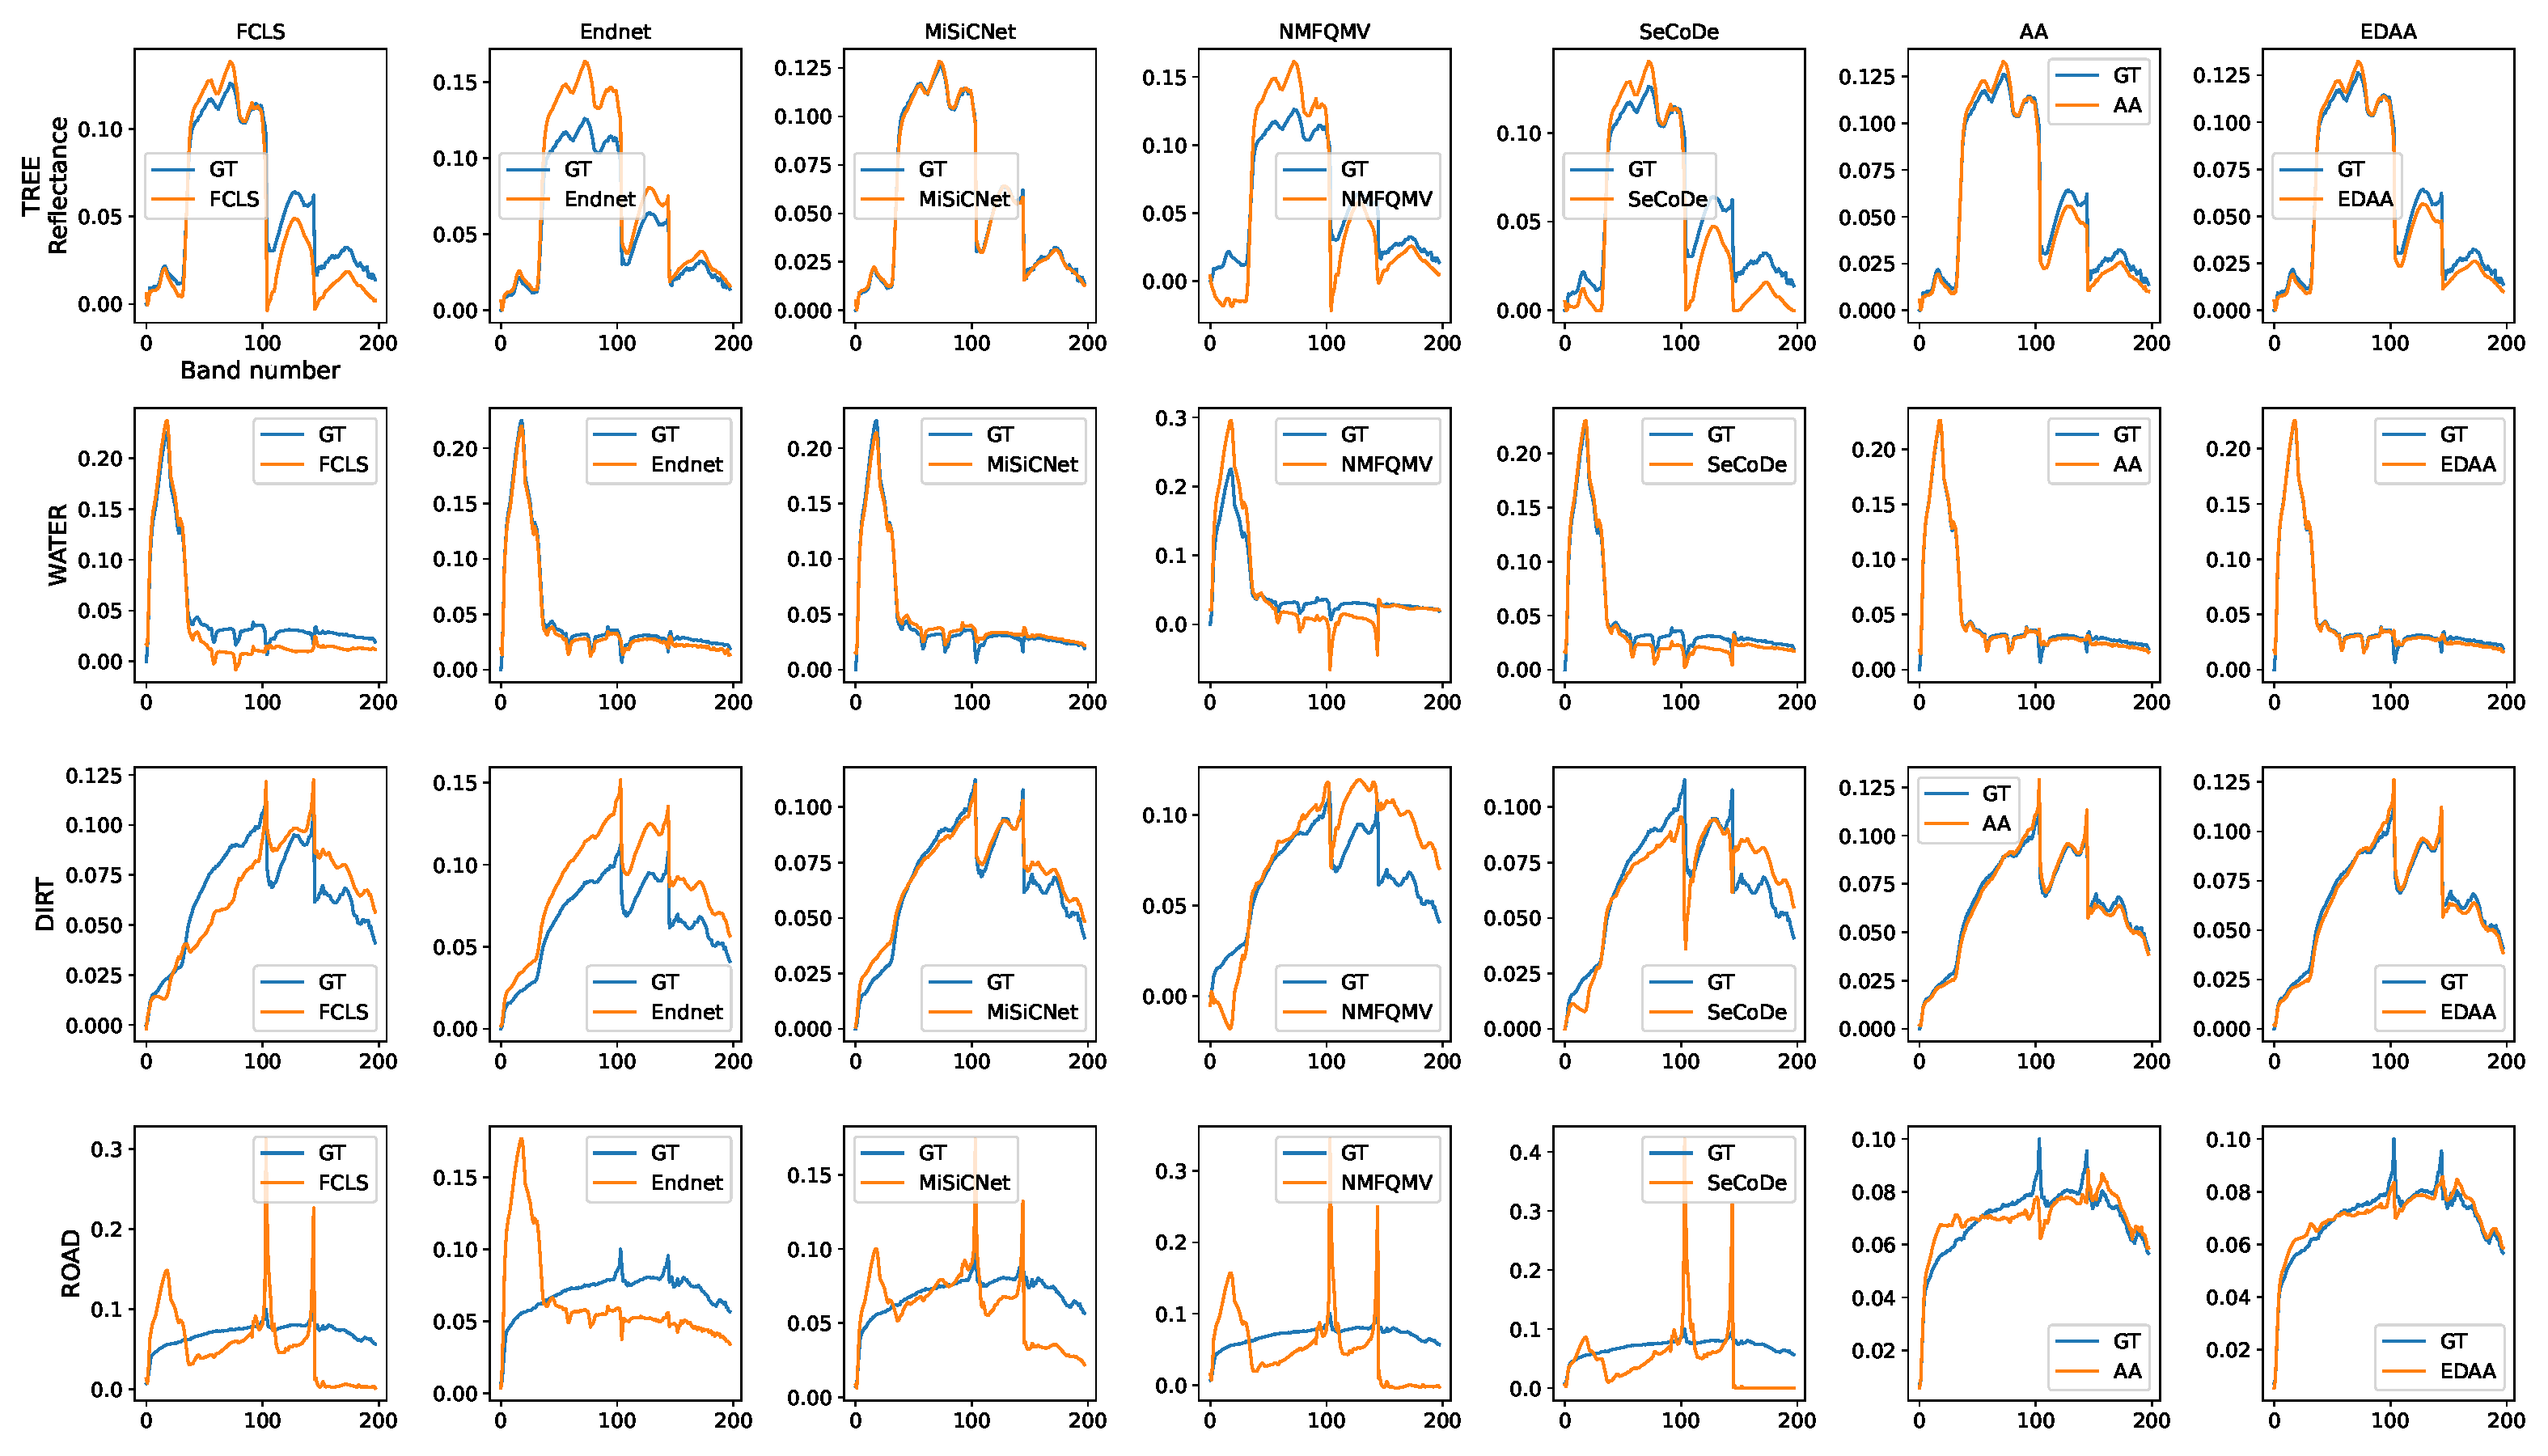
\includegraphics[width=\textwidth]{fichiers_latex/Chap2/figs/JasperRidgeE-final.pdf}}
  \hfil
  \centering
  \subfloat[]{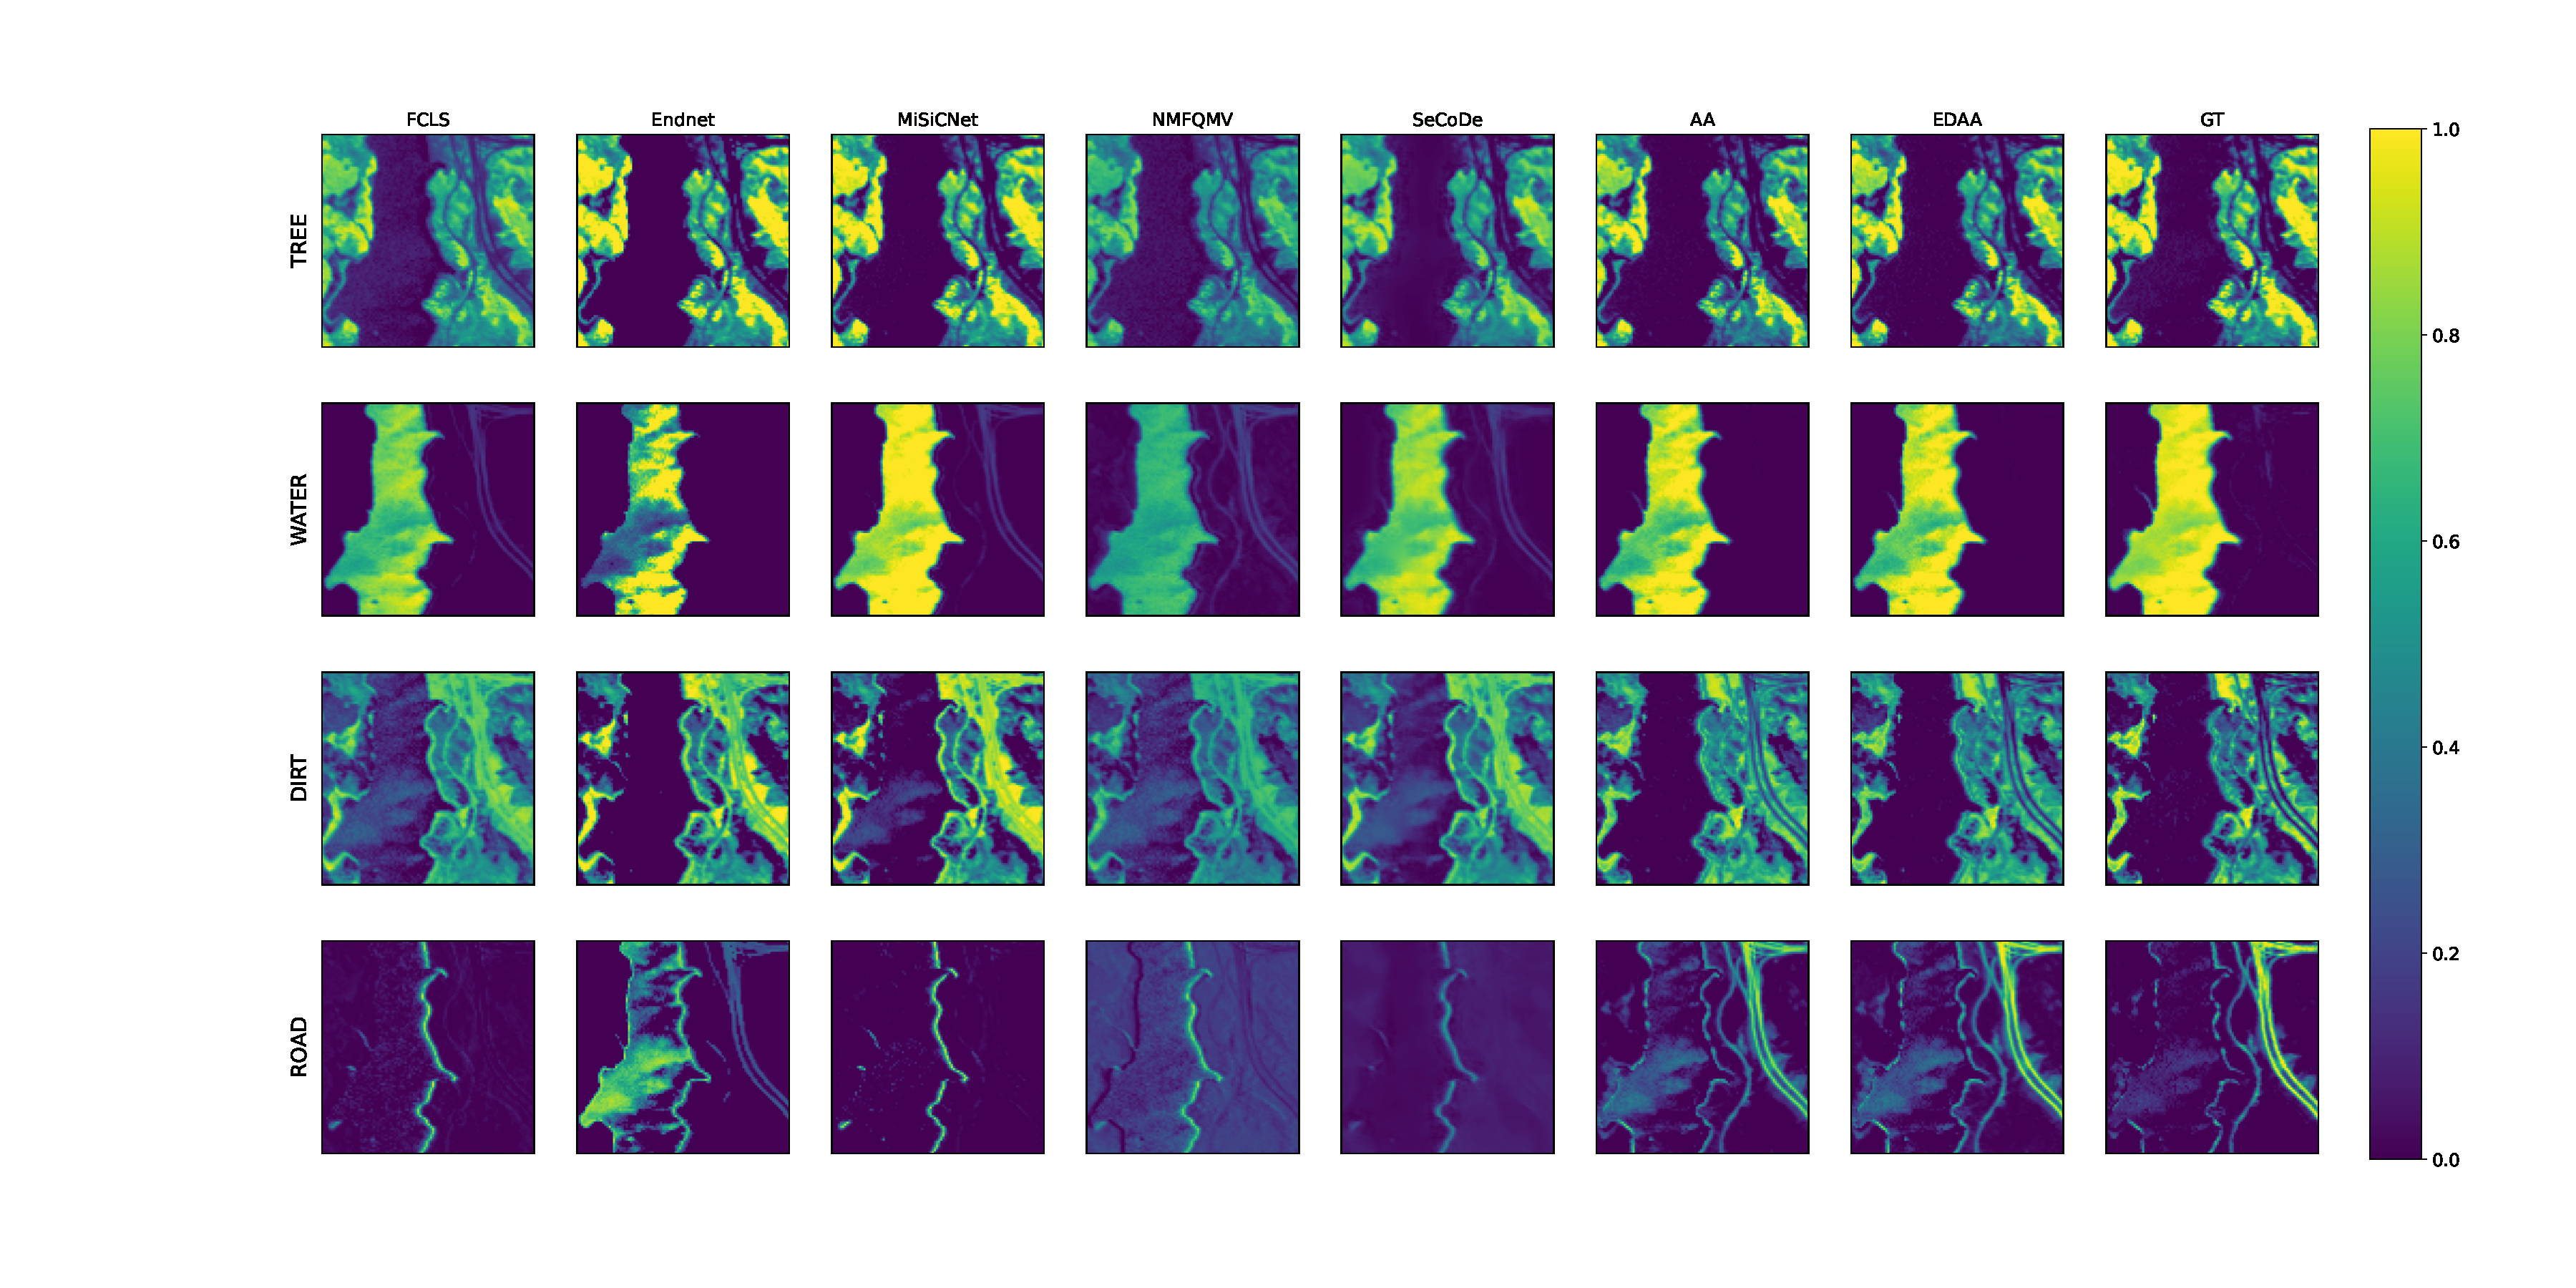
\includegraphics[width=\textwidth]{fichiers_latex/Chap2/figs/JasperRidgeA-final.pdf}}
  \caption{\rev{Estimated endmembers (a) and abundances (b) on the Jasper Ridge dataset.  Ground truth abundances are displayed on the right-most column.}}
  \label{fig:JR}
\end{figure}


\begin{figure}[h]
  \centering
  \subfloat[]{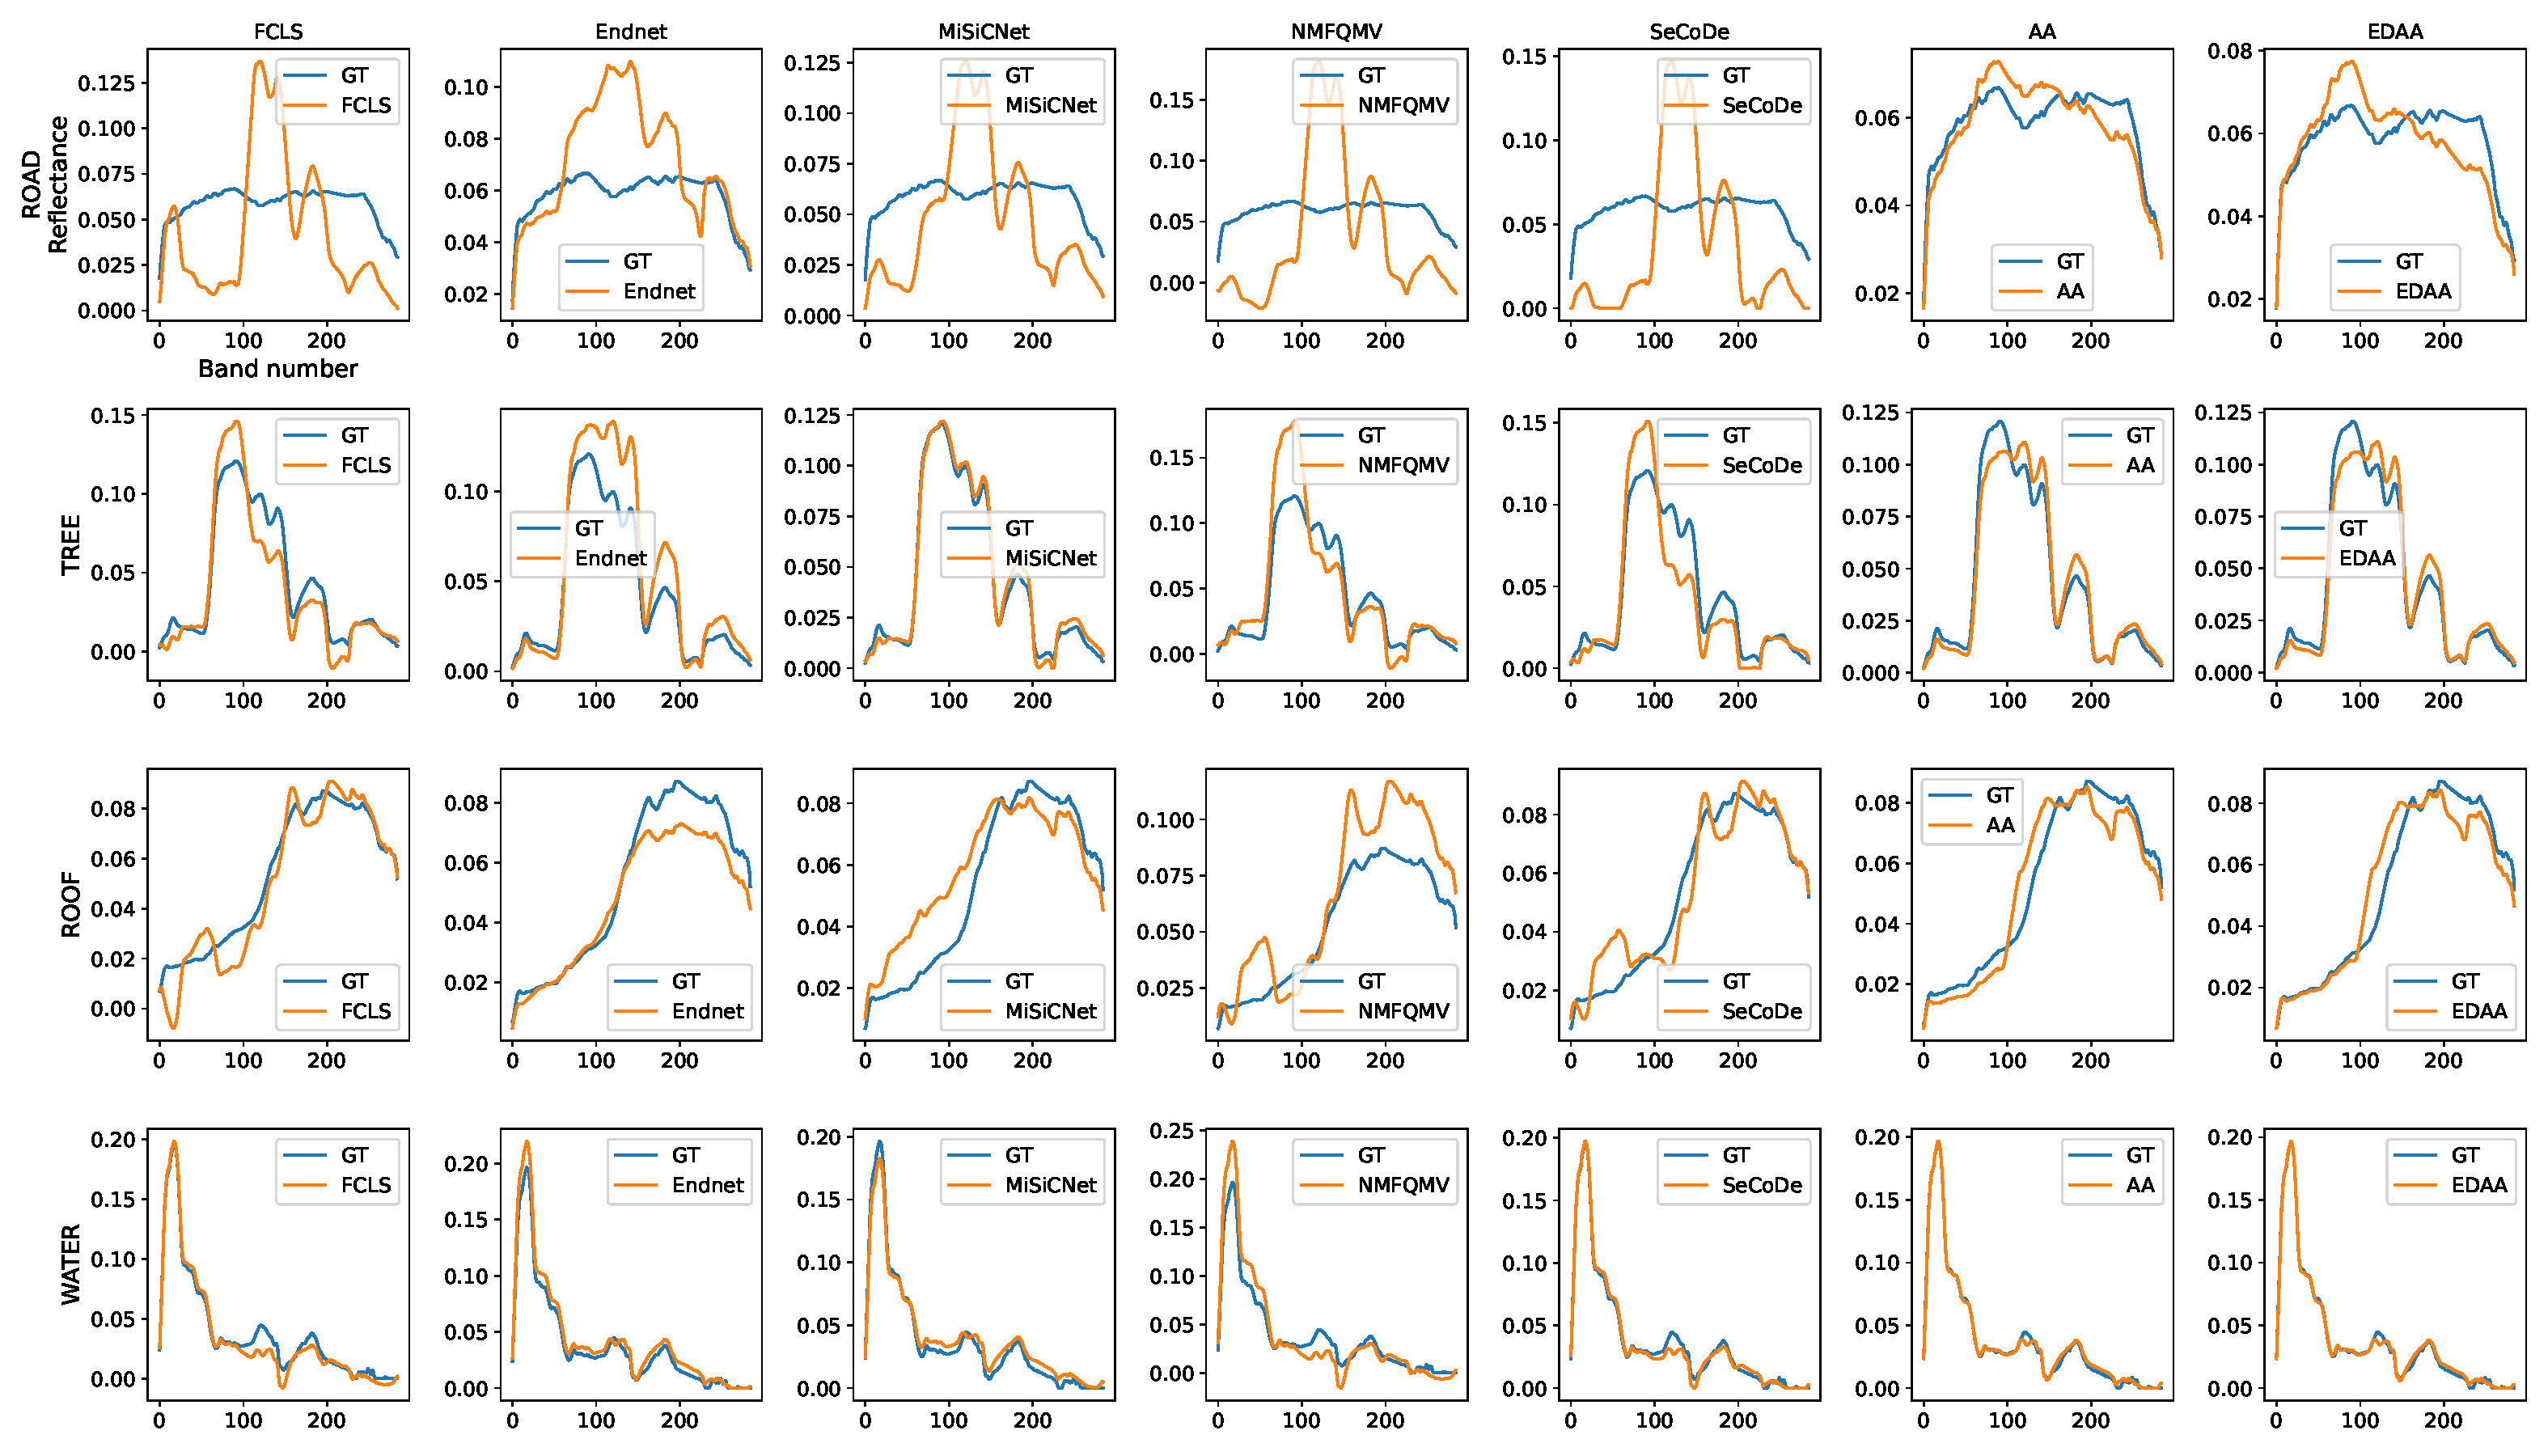
\includegraphics[width=\textwidth]{fichiers_latex/Chap2/figs/ApexE-final.pdf}}
  \hfil
  \subfloat[]{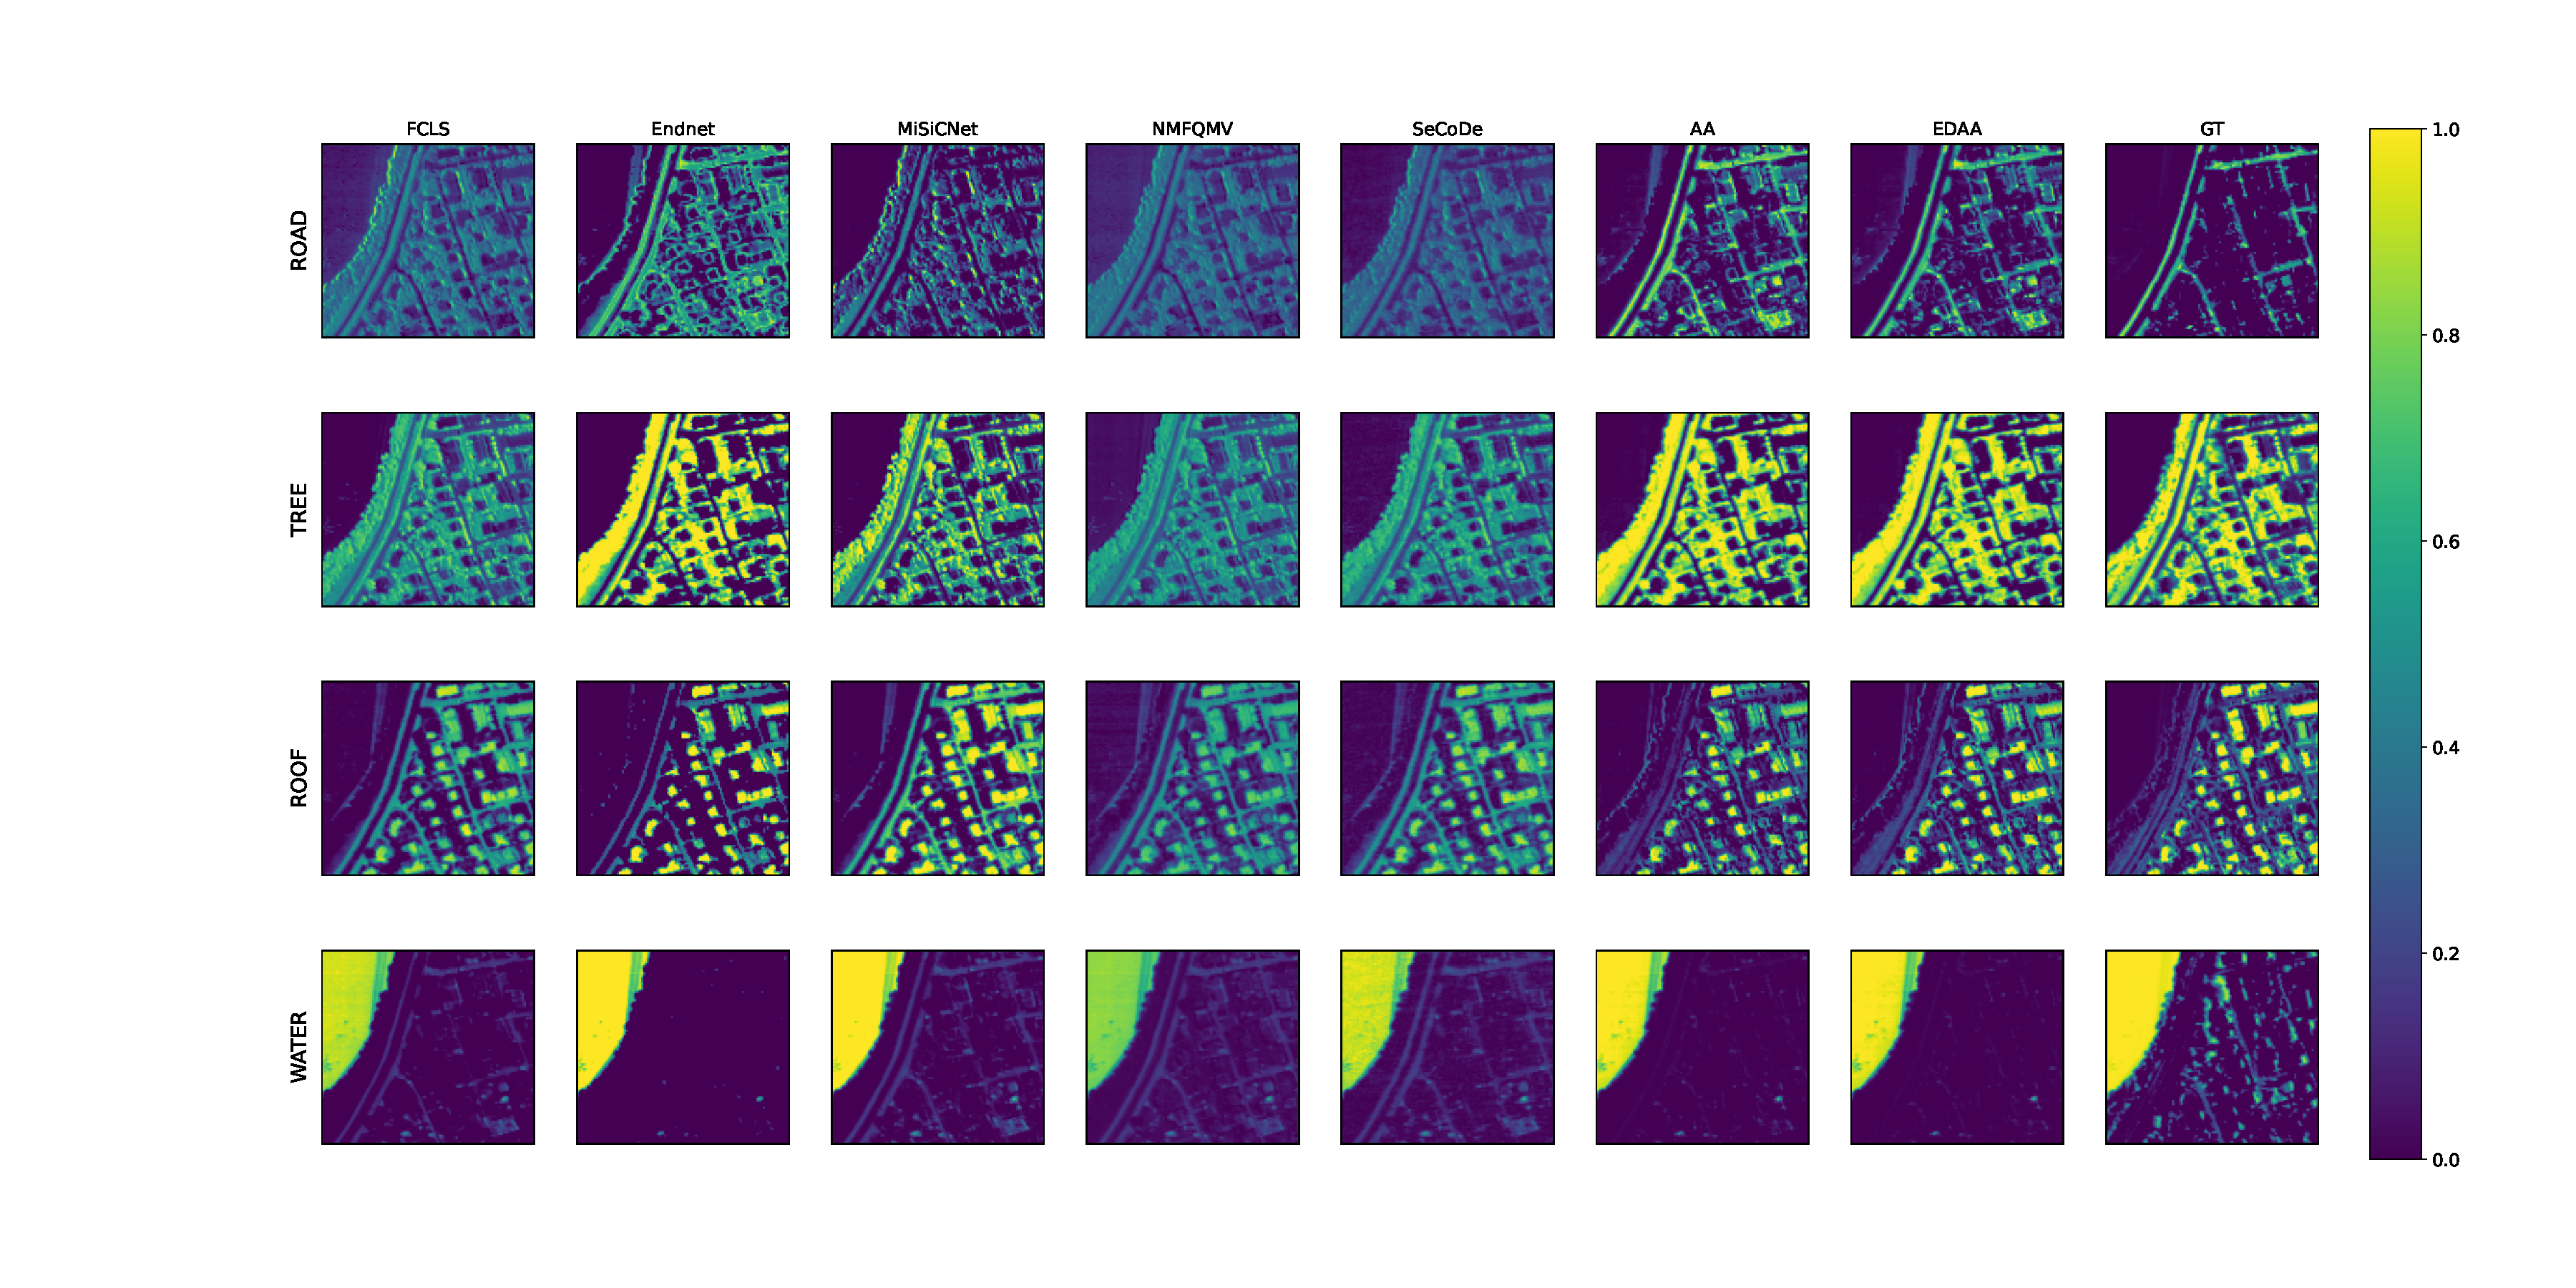
\includegraphics[width=\textwidth]{fichiers_latex/Chap2/figs/ApexA-final.pdf}}
  \caption{\rev{Estimated endmembers (a) and abundances (b) on the APEX dataset. Ground truth abundances are displayed on the right-most column.}}
  \label{fig:APEX}
\end{figure}

\begin{figure}[h]
  \centering
  \subfloat[]{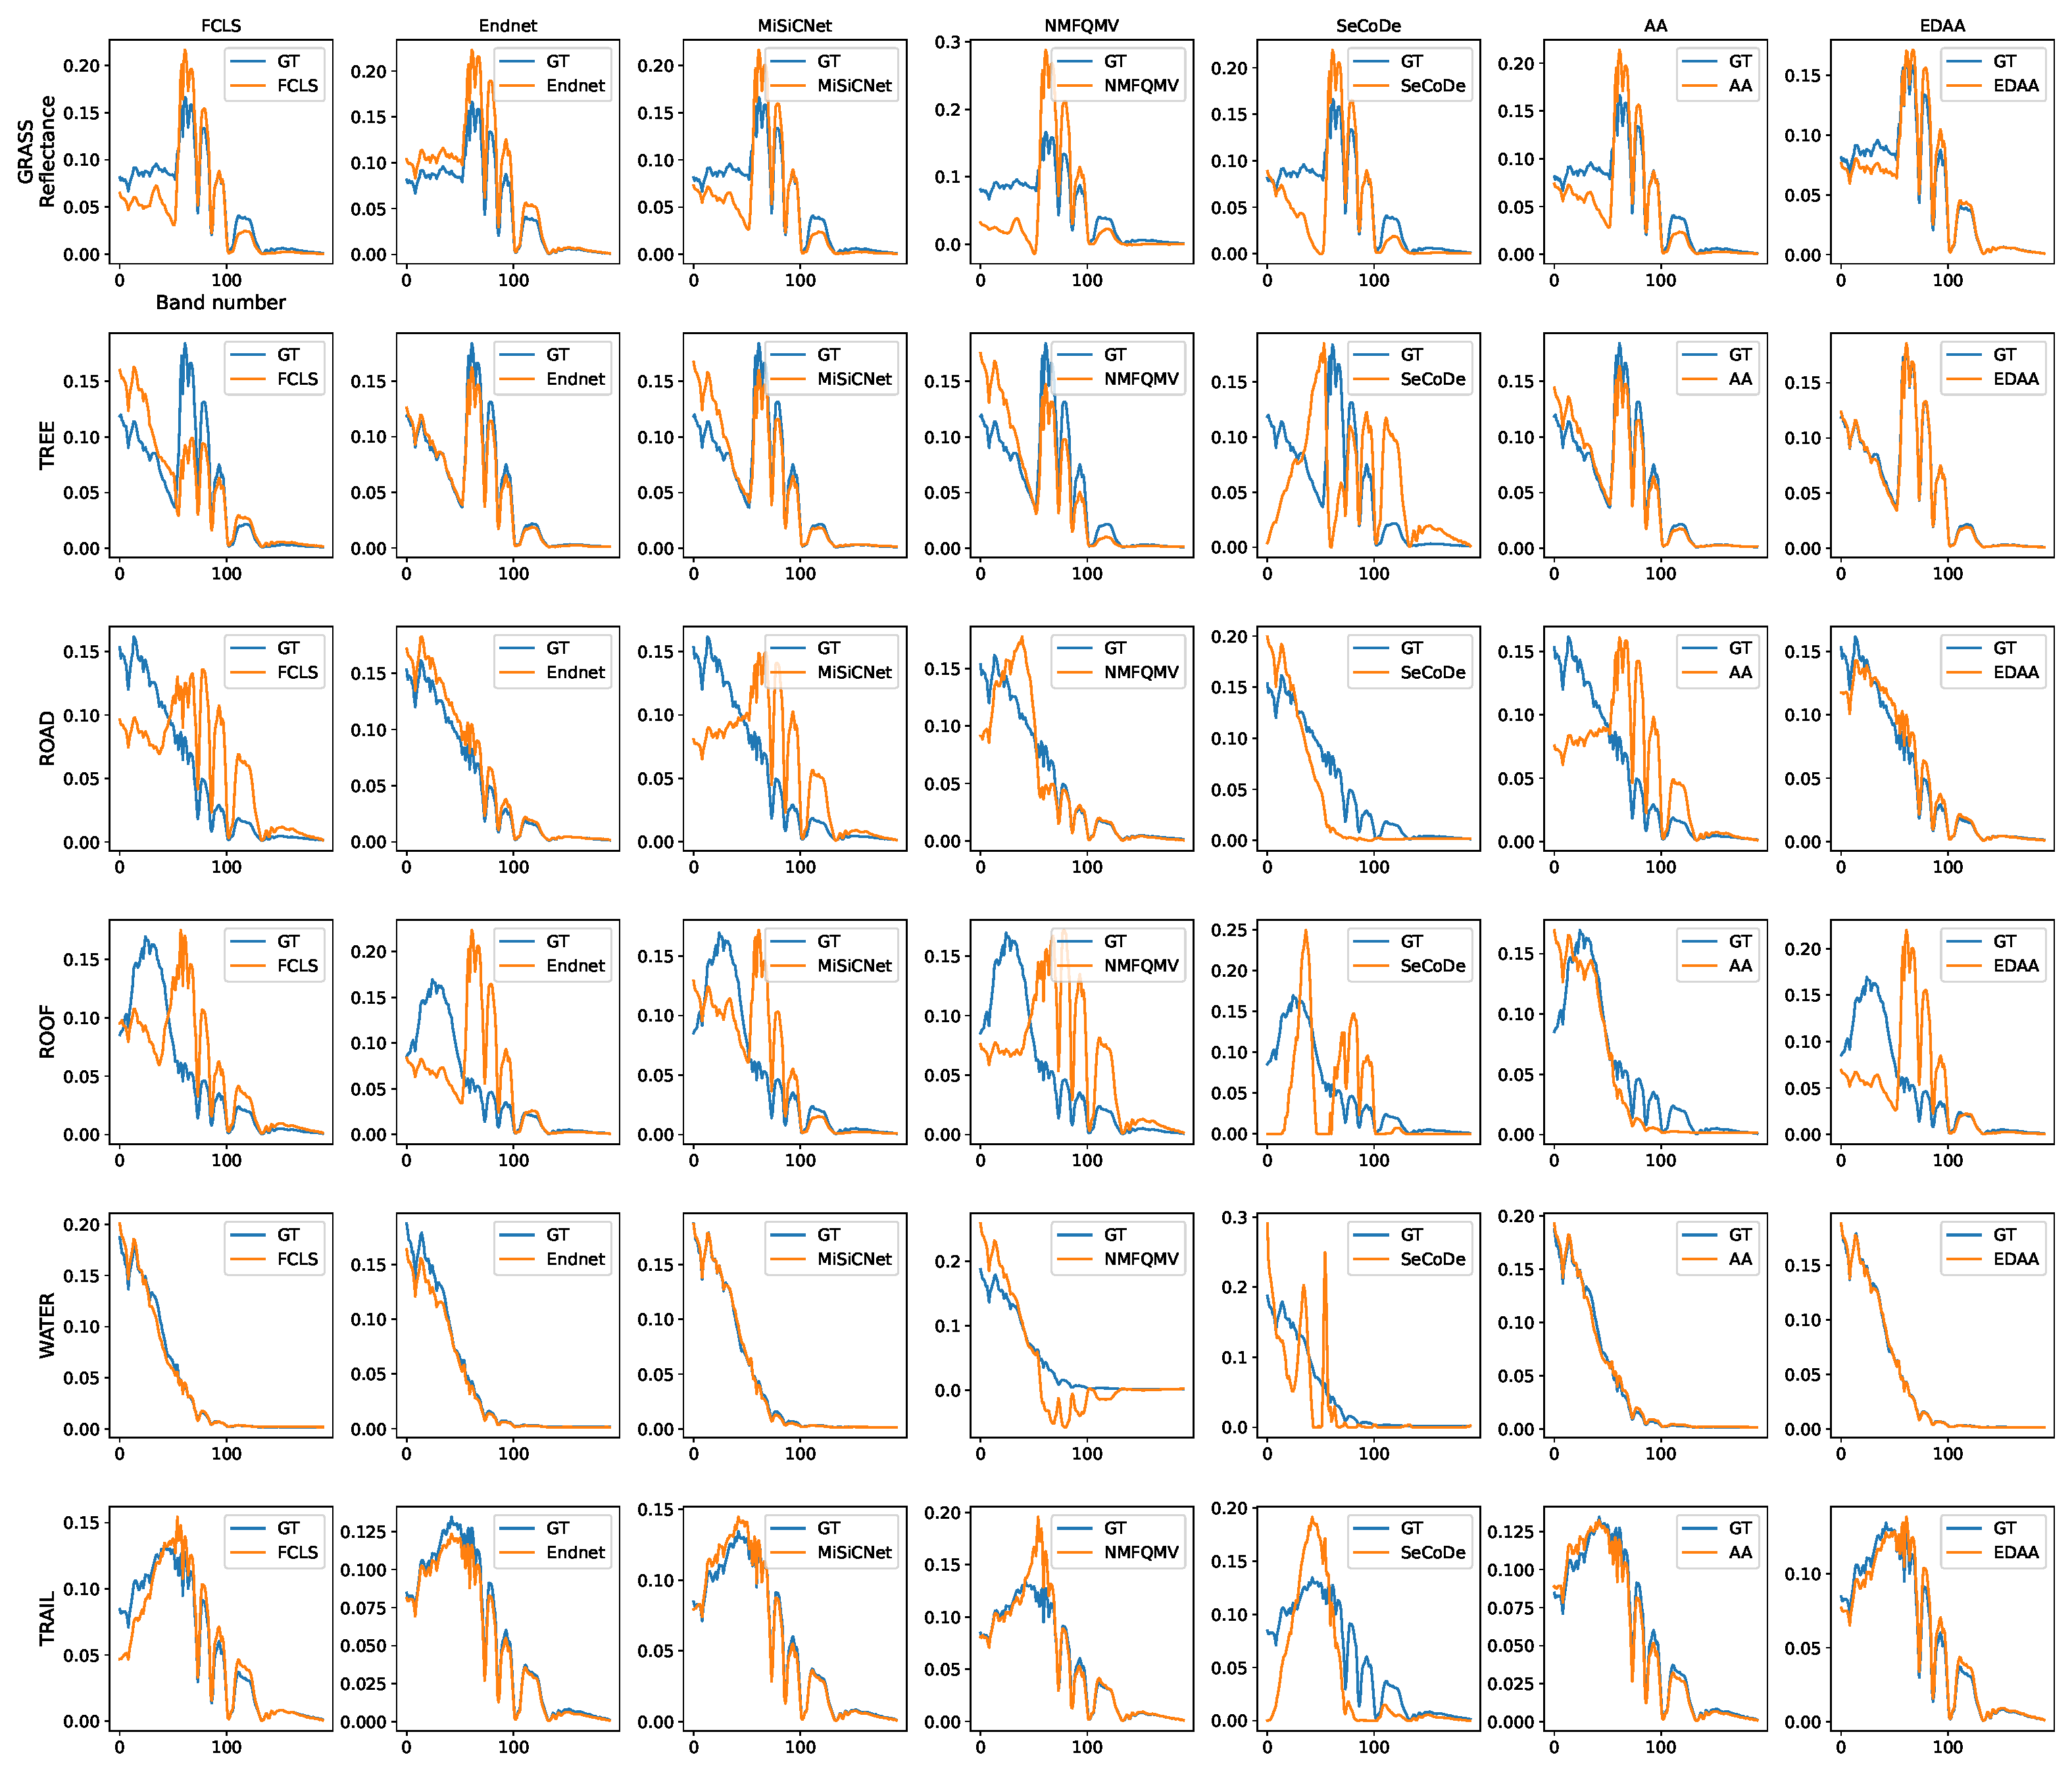
\includegraphics[width=0.66\textwidth]{fichiers_latex/Chap2/figs/WDCE-final.pdf}}
  \hfil
  \subfloat[]{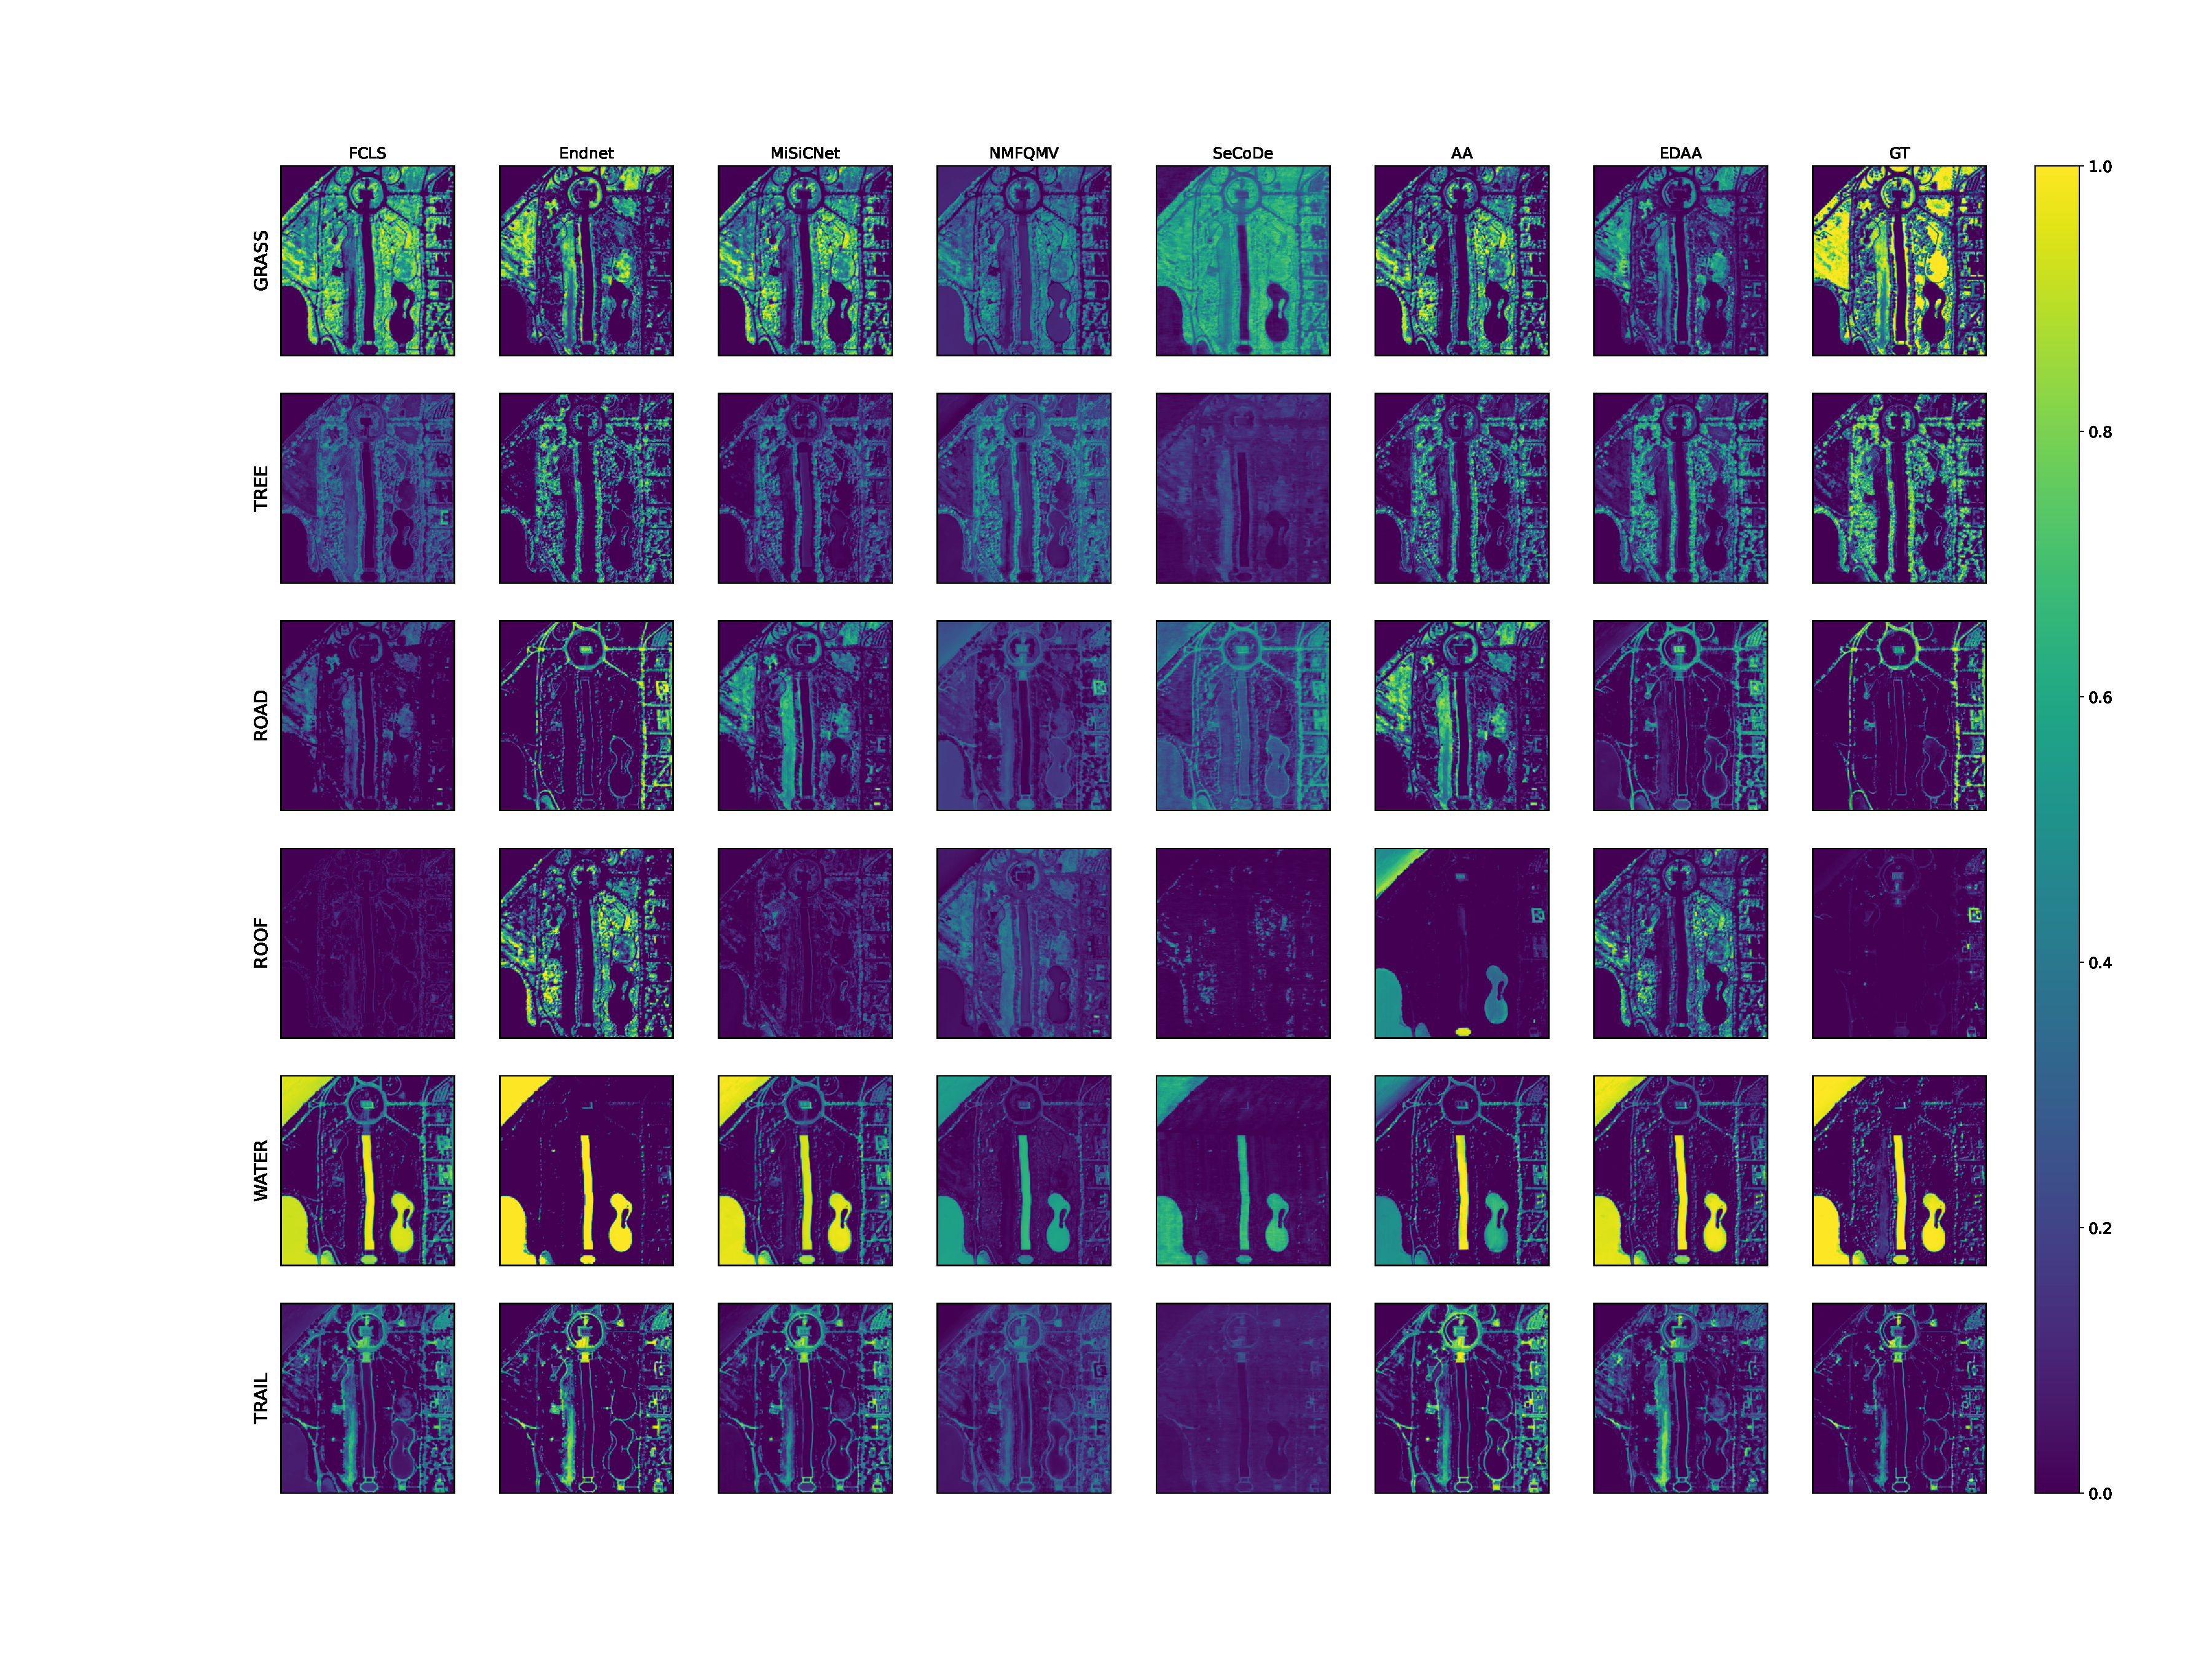
\includegraphics[width=\textwidth]{fichiers_latex/Chap2/figs/WDCA-final.pdf}}
  \caption{\rev{Estimated endmembers (a) and abundances (b) on the WDC dataset.  Ground truth abundances are displayed on the right-most column.}}
  \label{fig:WDC}
\end{figure}

Tables \ref{table:RMSE} and \ref{table:SAD} report the unmixing accuracy in
terms of abundances RMSE (\ref{eq:RMSE}) and endmembers SAD (\ref{eq:SAD}) on
six standard real datasets.
The datasets are arbitrarily ranked based on their difficulty.
For a fair comparison, all methods were evaluated on the $\ell_2$-normalized
data (\ref{eq:normalization}) which induces slight changes compared to the
results reported in \cite{rasti_misicnet_2022}.

\revision{Overall EDAA obtains the best abundances RMSE on five out of six real datasets. The results on Urban6 fall in favor of plain AA but the gap is moderate (12.83 vs 13.63) given that EDAA is more than seven times faster (594 versus 75 seconds) than plain AA on this dataset (see table \ref{table:cost}).}

\revision{Note however that plain AA performs poorly on WDC where the ground truth endmembers are highly correlated.}
We argue that our model selection technique is instrumental in avoiding
collapsing runs in which endmembers spectra are highly correlated.
This is underlined by the overall competitive SAD results obtained by EDAA
across datasets.
\revision{It should be noted that the SAD metric alone is not sufficient to assess the unmixing performance as a good SAD score does not necessarily lead to better abundance maps.
Thus it is not contradictory to have slightly worse SAD scores yet better looking abundance maps.}

The FCLS baseline based on VCA obtains rather poor results except for WDC.
This is likely due to the pure pixel assumption. Indeed, VCA selects a single
pixel to represent the endmembers spectra, which is too stringent in real
scenarios where spectral variability is ubiquitous.

Despite its quadratic minimum volume \emph{boundary} term, NMF-QMV generally
obtains worse results than the FCLS baseline.
Since it operates the unmixing in a subspace, NMF-QMV cannot prevent the endmembers spectra from having negative
values, which breaks the physical interpretability of the estimates and
subsequently harms the unmixing performance.
This phenomenon can be observed in figures
\ref{fig:JR},
\ref{fig:APEX} and \ref{fig:WDC} for
several endmembers.
The associated abundances show that NMF-QMV produces maps that are too uniform and lack sparsity.

\rev{In contrast, MVCNMF is a strong baseline as it does not operate in a subspace.}

When it comes to deep learning based methods, Endnet achieves very good results in terms of SAD but tends to
create overly sparse abundances which hinders its performance in terms of
abundances RMSE.
For instance, as can be seen in figure~\ref{fig:JR}, the
Road endmember is overlooked by Endnet even though EDAA recovers it neatly.
Likewise, in figure~\ref{fig:APEX}, the Road endmember spreads too much
compared to EDAA which appears closer to the ground truth.

MiSiCNet gives better unmixing results than Endnet in terms of abundances RMSE
except for APEX although the SAD results falls in favor of Endnet except for
Jasper Ridge.
This is likely due to Endnet using the spectral angle distance on
the input data in its loss which helps in achieving better SAD accuracy.
However a good SAD is not sufficient to obtain good abundance maps, an area
where MiSiCNet tends to shine as it incorporates spatial information by using
convolutional filters and implicitly applying a regularizer on abundances.

\rev{ADMMNet obtains rather poor results on all datasets, which is likely due to using ADMM to blindly solve 
the linear mixing model rather than leveraging a known library.}

\rev{SeCoDe works reasonably well on the Samson dataset due to its implementation available online that has been tailored to this dataset. However it does not perform as well on other datasets, which is likely due to requiring precise hyperparameters tuning depending on the data at hand.}

\rev{NCAA obtains reasonable results due to its fine-tuning procedure but its computational cost is prohibitive as we will be discussing next.}

\revision{Finally, the plain AA method leveraging an active-set algorithm is a very competitive method for five out of six datasets, yet its performance drops significantly when dealing with the hardest mixing scenario that is WDC.}

For example, in figure~\ref{fig:JR} only
AA and EDAA are able to uncover the Road endmember in Jasper
Ridge whereas all the other techniques fail.

\revision{Unlike EDAA, AA does not rely on a random initialization of the estimates as they are set to zeros in practice. 
Instead, EDAA requires starting from feasible points w.r.t. the optimization sub-problems.
In addition, the initial estimates in EDAA should not contain any zeros due to the presence of the logarithm in 
(\ref{eq:update_EDAA_softmax2}).
Thanks to the entropic gradient descent speed, it is possible to fit several models that have been randomly initialized as described in \ref{subsec:details} and use the model selection procedure presented in Algorithm \ref{alg:criterion} which selects the model that exhibits the lowest coherence among the pool of candidates that are well fitted.
Notably, this approach prevents the estimated endmembers from \emph{collapsing} into degenerate solutions that would end up being perfectly correlated.
This likely explains why the performance of plain AA on WDC drops as the endmembers are highly correlated.
}

\rev{Additional qualitative results for the Samson, Urban4 and Urban6 datasets can be found
in the supplementary material.}
\revision{Moreover, we have also included the results on a 250$\times$191 pixels subset of the Cuprite dataset, which is more challenging and does not come with ground truth abundance maps.}

\subsection{Computational cost}

Table \ref{table:cost} reports the processing times for the different unmixing
algorithms on the six real datasets. 
\rev{MVCNMF, NMF-QMV, SeCoDe and NCAA were implemented in Matlab (2020b) while
FCLS, Endnet, MiSiCNet, ADMMNet and the AA variants were implemented in Python (3.8).
NMF-QMV, MVCNMF, SeCoDe, NCAA, FCLS and AA run on CPU whereas Endnet, MiSiCNet, ADMMNet and EDAA run on GPU.}
The processing times were obtained using a computer with an Intel(R) Xeon(R)
Silver 4110 processor (2.10 GHz), 32 cores, 64GB of memory, and a NVIDIA
GeForce RTX (2080 Ti) graphical processing unit.
The table shows that FCLS is clearly faster than the other unmixing techniques,
however it is a supervised method that relies on an endmembers extraction
algorithm. In this case, VCA is used which is also fast.
The deep learning methods are the slowest techniques despite running on GPU.
Interestingly, EDAA requires a lower computational cost than NMF-QMV and AA although our approach consists in aggregating 50 runs obtained
iteratively. 
For example, it takes on average 1.5 seconds for EDAA to perform a single unmixing
task on the Urban6 dataset, which is three times faster than FCLS. 
This demonstrates the efficiency of EDAA which allows us to use an
adequate model selection procedure over several runs.
\rev{Note that the processing time of NCAA is prohibitive due to its fine-tuning component despite using a fast projected gradient method.}

\begin{table*}[h]
  \centering
  \captionof{table}{Processing times in seconds on six real datasets. The best
    results are in bold and the second best underlined. EDAA includes the model
    selection procedure over $M=50$ runs.}
  \begin{adjustbox}{width=\textwidth}
    % \begin{tabular}{c | c c c c c c c}
%   \toprule
%   & FCLSU & Endnet & MiSiCNet & NMF-QMV & AA & RAA & EDAA \\
%   \hline
%   Samson & \textbf{0.3} & 560.0 & 80.0 & 20.1 & 17.6 & 16.4 & \underline{11.2} \\
%   JasperRidge & \textbf{0.4} & 680.0 & 90.0 & 22.3 & 21.9 & 21.1 & \underline{9.6} \\
%   Urban4 & \textbf{3.6} & 720.0 & 411.0 & 112.5 & 237.6 & 228.4 & \underline{66.3} \\
%   Urban6 & \textbf{4.4} & 1000.0 & 417.0 & 158.4 & 343.0 & 327.9 & \underline{75.2} \\
%   APEX & \textbf{0.6} & 720.0 & 92.0 & 27.2 & 44.8 & 31.0 & \underline{15.4} \\
%   WDC & \textbf{4.0} & 1000.0 & 409.0 & 174.4 & 361.8 & 324.7 & \underline{81.0} \\
%   \bottomrule
% \end{tabular}

% Remove RAA


%\begin{tabular}{c | c c c c c c}
%  \toprule
%  & FCLSU & Endnet & MiSiCNet & NMF-QMV & AA & EDAA \\
%  \hline
%  Samson & \textbf{0.3} & $\approx$ 560 & $\approx$ 80 & 20.1 & 17.6 & \underline{11.2} \\
%  JasperRidge & \textbf{0.4} & $\approx$ 680 & $\approx$ 90 & 22.3 & 21.9 & \underline{9.6} \\
%  Urban4 & \textbf{3.6} & $\approx$ 720 & $\approx$ 411 & 112.5 & 237.6 & \underline{66.3} \\
%  Urban6 & \textbf{4.4} & $\approx$ 1000 & $\approx$ 417 & 158.4 & 343.0 & \underline{75.2} \\
%  APEX & \textbf{0.6} & $\approx$ 720 & $\approx$ 92 & 27.2 & 44.8 & \underline{15.4} \\
%  WDC & \textbf{4.0} & $\approx$ 1000 & $\approx$ 409 & 174.4 & 361.8 & \underline{81.0} \\
%  \bottomrule
%\end{tabular}

% Recompute AA with T=100

\begin{tabular}{c | c c c c c c c c | c c}
  \toprule
  & FCLS & Endnet & MiSiCNet & \rev{ADMMNet} & \rev{MVCNMF} & NMF-QMV & \rev{SeCoDe} & \rev{NCAA} & \revision{AA ($T=100$)} & EDAA \\
  \hline
  Samson & \textbf{0.3} & $\approx$ 560 & $\approx$ 80 & 55.2 & \underline{3.8} & 20.1 & 24.2 & 113.1 & \revision{33.0} & 11.2 \\
  JasperRidge & \textbf{0.4} & $\approx$ 680 & $\approx$ 90 & 54.1 & \underline{8.0} & 22.3 & 28.6 & 501.4 & \revision{43.6} & 9.6 \\
  Urban4 & \textbf{3.6} & $\approx$ 720 & $\approx$ 411 & 504.6 & \underline{25.4} & 112.5 & 475.1 & 3529.9 & \revision{415.7} & 66.3 \\
  Urban6 & \textbf{4.4} & $\approx$ 1000 & $\approx$ 417 & 507.5 & \underline{45.0} & 158.4 & 707.7 & 4880.8 & \revision{593.7} & 75.2 \\
  APEX & \textbf{0.6} & $\approx$ 720 & $\approx$ 92 & 80.0 & \underline{11.3} & 27.2 & 56.1 & 441.5 & \revision{75.4} & 15.4 \\
  WDC & \textbf{4.0} & $\approx$ 1000 & $\approx$ 409 & 535.8 & \underline{55.1} & 174.4 & 524.7 & 4179.0 & \revision{493.1} & 81.0 \\
  \bottomrule
\end{tabular}






  \end{adjustbox}
  \label{table:cost}
\end{table*}

\subsection{Ablation study}

Finally, we study the sensitivity to hyper-parameters for Algorithm \ref{alg:EDAA} and
\ref{alg:criterion} in figure \ref{fig:ablation} where the Y-axis corresponds to the
overall abundances RMSE.
Given a fixed computational budget of 1000 updates, figure \ref{fig:ablation}
(a) shows that the hyper-parameters of EDAA are robust provided that the number
of runs $M$ in the model selection is large enough (here 100). Only the two extremes
configurations ($K_1=K_2=1$, $T=500$ and $K_1=K_2=50$, $T=10$) are slightly
worse, especially on Urban6.
For the remaining experiments, we use $K_1=K_2=5$.
In figure \ref{fig:ablation} (b), we see that the number of outer iterations is
quite stable except for WDC which requires more updates (1000, \ie $T=100$).
Finally, we study the importance of the number of runs $M$ from which to select
the best candidate in figure \ref{fig:ablation} (c).
We observe that the model selection procedure requires at least 50 runs to
obtain very good performances, hence we use $M=50$ in our unmixing experiments.
On unknown datasets where real-time unmixing is not required, it is advised to
use a large number of runs (at least 100) to ensure that the model selection
procedure yields a good candidate.
Detailed results for both abundances RMSE and SAD metrics are available in the
supplementary material.

\begin{figure}[]
  \centering
  \subfloat[]{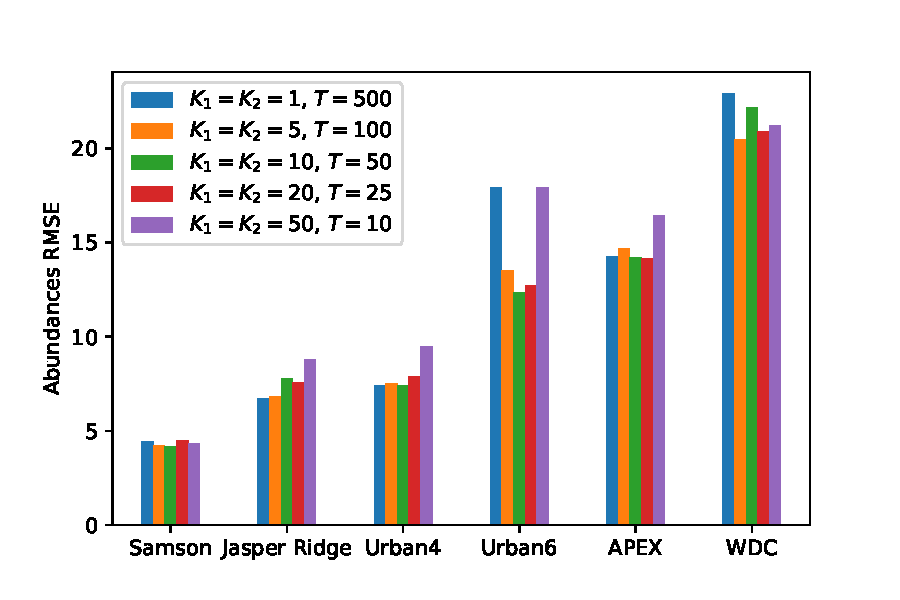
\includegraphics[width=0.33\textwidth]{fichiers_latex/Chap2/figs/alg1_constant.pdf}}
  \hfil
  \subfloat[]{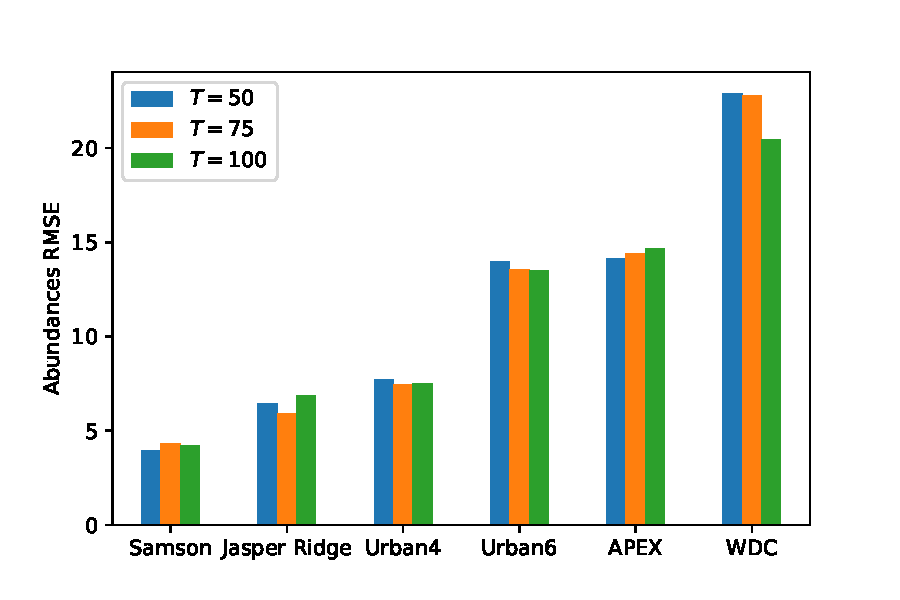
\includegraphics[width=0.33\textwidth]{fichiers_latex/Chap2/figs/alg1_T.pdf}}
  \hfil
  \subfloat[]{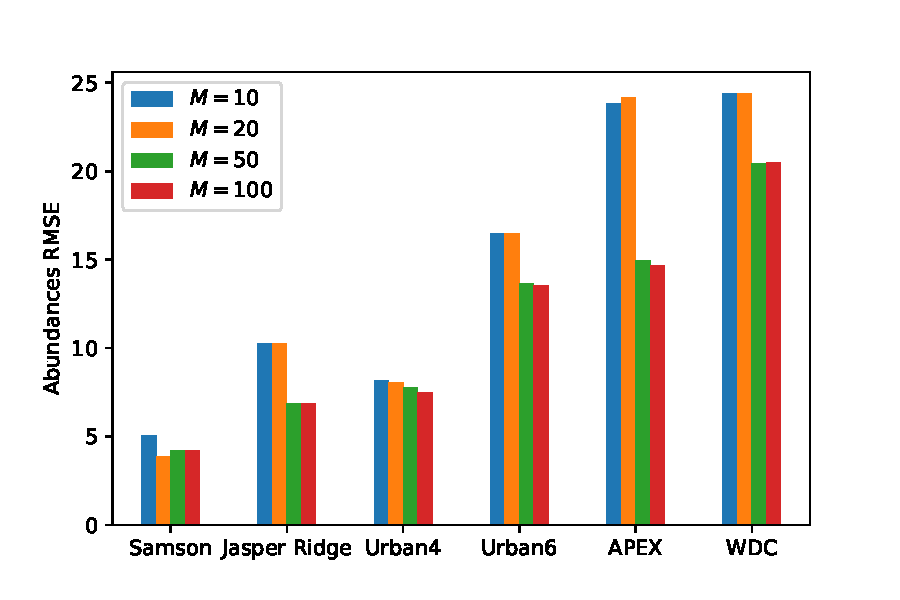
\includegraphics[width=0.33\textwidth]{fichiers_latex/Chap2/figs/alg2.pdf}}
  \caption{Sensitivity analysis to the hyperparameters in Algorithms
    \ref{alg:EDAA} and \ref{alg:criterion} measured in global abundances RMSE: (a) Varying
  inner and outer iterations $K_1, K_2$ and $T$ for a constant number of updates
  (1000) and runs $M=100$, (b) Varying
outer iterations $T$ using $K_1=K_2=5$ and (c) Varying number of runs $M$ using
$K_1=K_2=5$ and $T=100$.}
  % \caption{Samson dataset: (a) False colors RGB image (Red: 83rd band, Green: 43, Blue: 9) (b)
  % $\ell_2$-normalized ground truth endmembers.}
  \label{fig:ablation}
\end{figure}

\section{Conclusion}
\label{sec:EDAA_ccl}

We have proposed a new algorithm based on archetypal analysis for blind
hyperspectral unmixing.
We have shown how to take advantage of its efficient GPU implementation in order
to develop an adequate model selection procedure to obtain state-of-the-art
performances.
Remarkably, our simple and easy-to-use approach considerably improves the unmixing
results on a comprehensive collection of standard real datasets.
In addition, we have made our results reproducible by releasing an open source
codebase which also includes the plain archetypal analysis variant presented in this study.
\rev{While this paper was under review, we also investigated in~\cite{rasti_sunaa_2023} the problem of semi-supervised unmixing by using a variant of archetypal analysis, showing that such a framework may be useful beyond the problem of blind unmixing that we address here.}
\revision{Finally, it is worth noting that our approach does not consider the spatial structure of the data. This feature suggests that a natural extension to our approach would be to incorporate missing spatial information, which could potentially improve the accuracy of our results.}

\chapter*{Appendix}

\section{Datasets description}

In this section, we provide illustrations of the unmixing datasets
used in the experiments. Each dataset is described with a false-color RGB image
alongside the $\ell_2$-normalized ground truth endmembers.


  \begin{figure}[h]
    \centering
    \subfloat[]{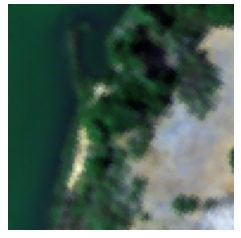
\includegraphics[height=1in]{fichiers_latex/Chap2/figs/SamsonY_GT.png}}
    \hfil
    \subfloat[]{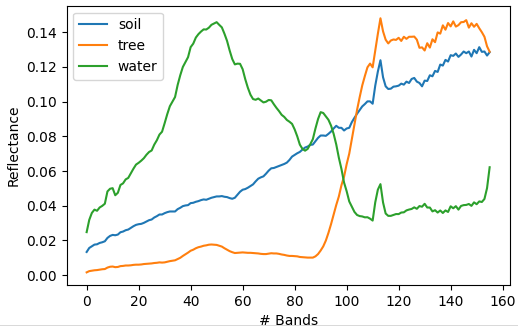
\includegraphics[height=1in]{fichiers_latex/Chap2/figs/SamsonE_GT.png}}
    \caption{Samson dataset: (a) False colors RGB image (Red: 83rd band, Green: 43, Blue: 9) (b)
    $\ell_2$-normalized ground truth endmembers.}
    \label{fig:samson}
  \end{figure}

  \begin{figure}[h]
    \centering
    \subfloat[]{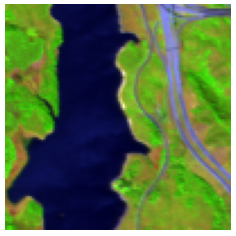
\includegraphics[height=1in]{fichiers_latex/Chap2/figs/JasperRidgeY_GT.png}}
    \hfil
    \subfloat[]{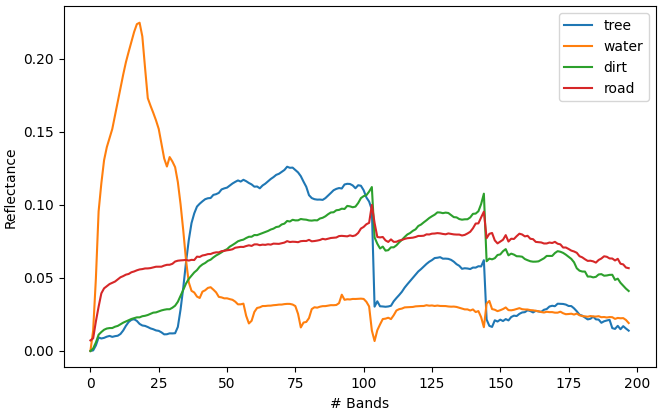
\includegraphics[height=1in]{fichiers_latex/Chap2/figs/JasperRidgeE_GT.png}}
    \caption{JasperRidge dataset: (a) False colors RGB image (Red: 130th band, Green: 50, Blue:
    5) (b) $\ell_2$-normalized ground truth endmembers.}
    \label{fig:jasper}
  \end{figure}

  \begin{figure}[h]
    \centering
    \subfloat[]{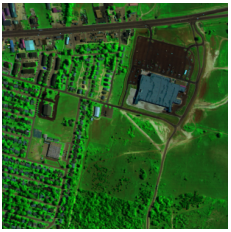
\includegraphics[height=1in]{fichiers_latex/Chap2/figs/UrbanY_GT.png}}
    \hfil
    \subfloat[]{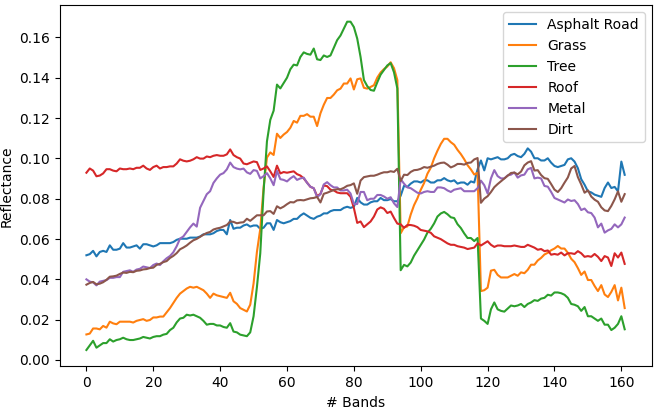
\includegraphics[height=1in]{fichiers_latex/Chap2/figs/Urban6E_GT.png}}
    \caption{Urban dataset: (a) False colors RGB image (Red: 130th band, Green: 70, Blue: 30) (b)
    $\ell_2$-normalized ground truth endmembers for Urban6. Urban4 corresponds to the first 4
    materials.}
    \label{fig:urban_GT}
  \end{figure}
  
  \begin{figure}[h]
    \centering
    \subfloat[]{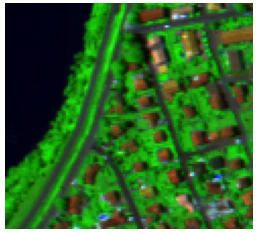
\includegraphics[height=1in]{fichiers_latex/Chap2/figs/APEXY_GT.png}}
    \hfil
    \subfloat[]{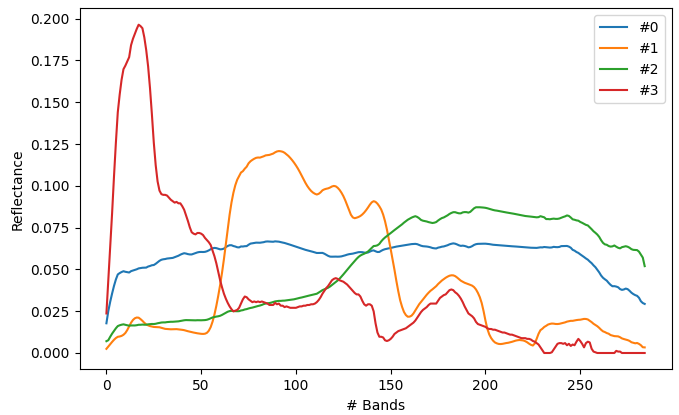
\includegraphics[height=1in]{fichiers_latex/Chap2/figs/APEXE_GT.png}}
    \caption{APEX dataset: (a) False colors RGB image (Red: 200th band, Green: 100, Blue: 10) (b)
    $\ell_2$-normalized ground truth endmembers (\#0: Road, \#1: Tree, \#2: Roof,
    \#3: Water).}
    \label{fig:apex}
  \end{figure}

  \begin{figure}[h]
    \centering
    \subfloat[]{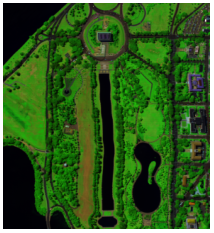
\includegraphics[height=1in]{fichiers_latex/Chap2/figs/WDCY_GT.png}}
    \hfil
    \subfloat[]{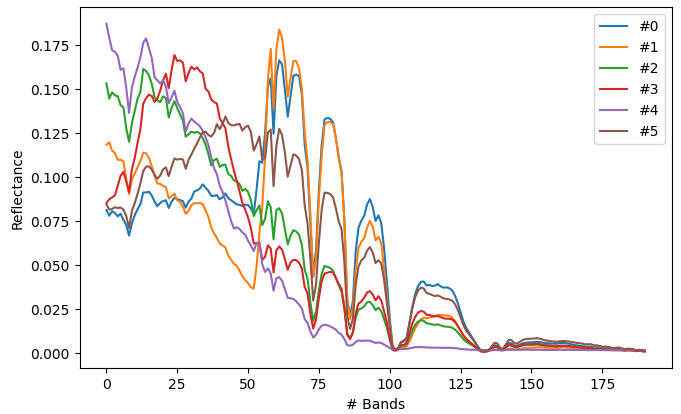
\includegraphics[height=1in]{fichiers_latex/Chap2/figs/WDCE_GT.png}}
    \caption{Washington DC Mall dataset: (a) False colors RGB image (Red: 150th band, Green: 75,
    Blue: 20) (b) $\ell_2$-normalized ground truth endmembers (\#0: Grass, \#1:
    Tree, \#2: Road, \#3: Roof, \#4: Water, \#5: Trail).}
    \label{fig:wdc}
  \end{figure}

\section{Additional results}

We provide qualitative results on the Samson, Urban4 and Urban6 datasets in figures~\ref{fig:Samson}, ~\ref{fig:Urban4} and ~\ref{fig:Urban6}.

\begin{figure}[h]
  \centering
  \subfloat[]{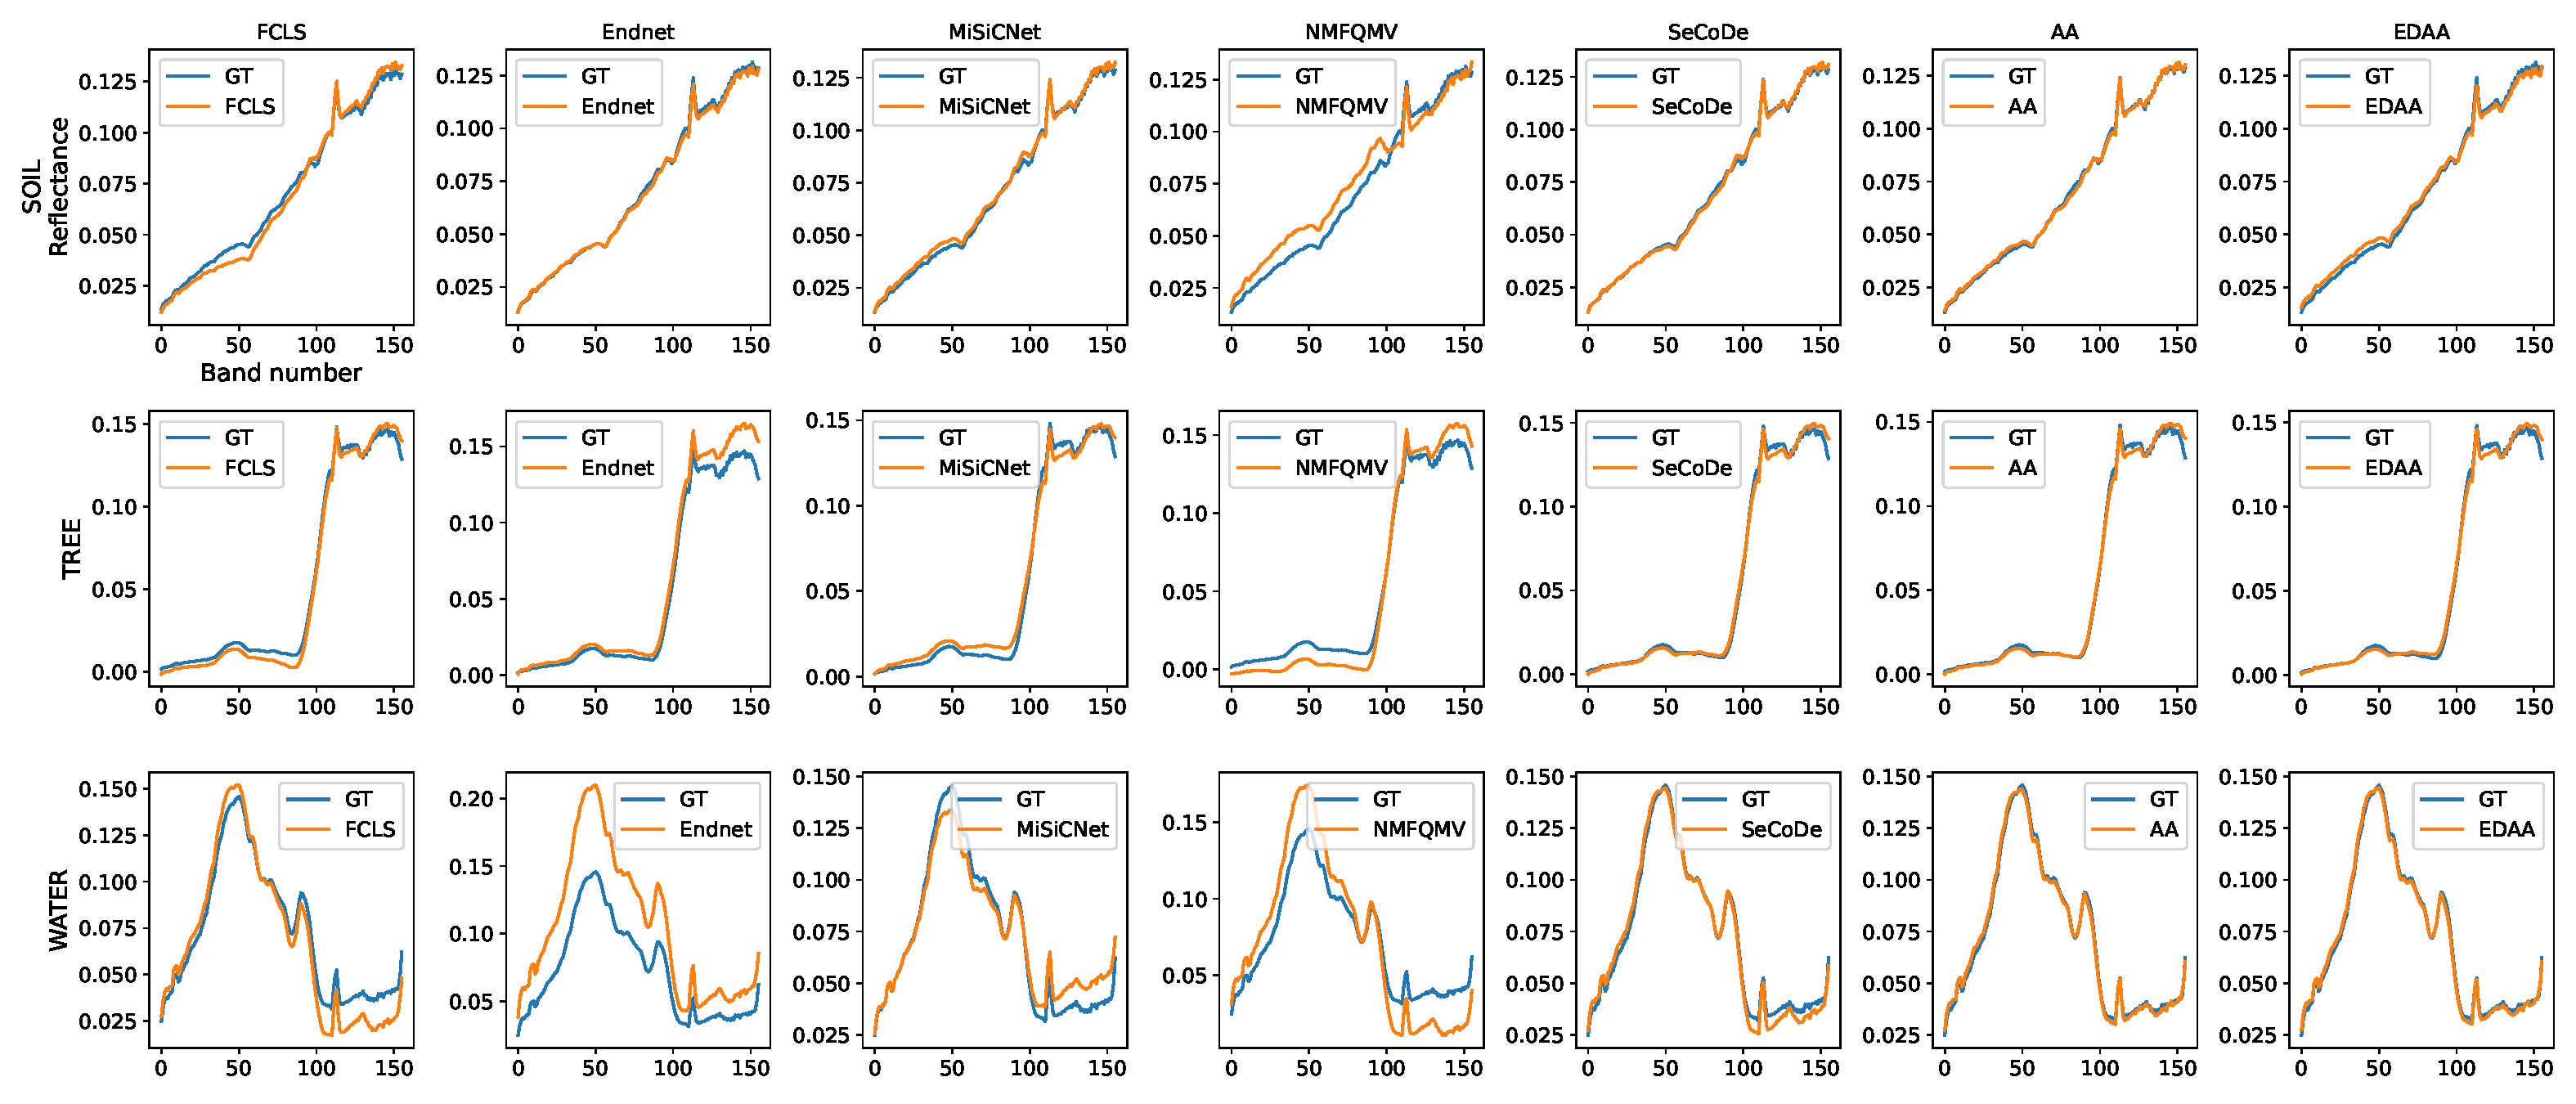
\includegraphics[width=\textwidth]{fichiers_latex/Chap2/figs/SamsonE-final.pdf}}
  \hfil
  \subfloat[]{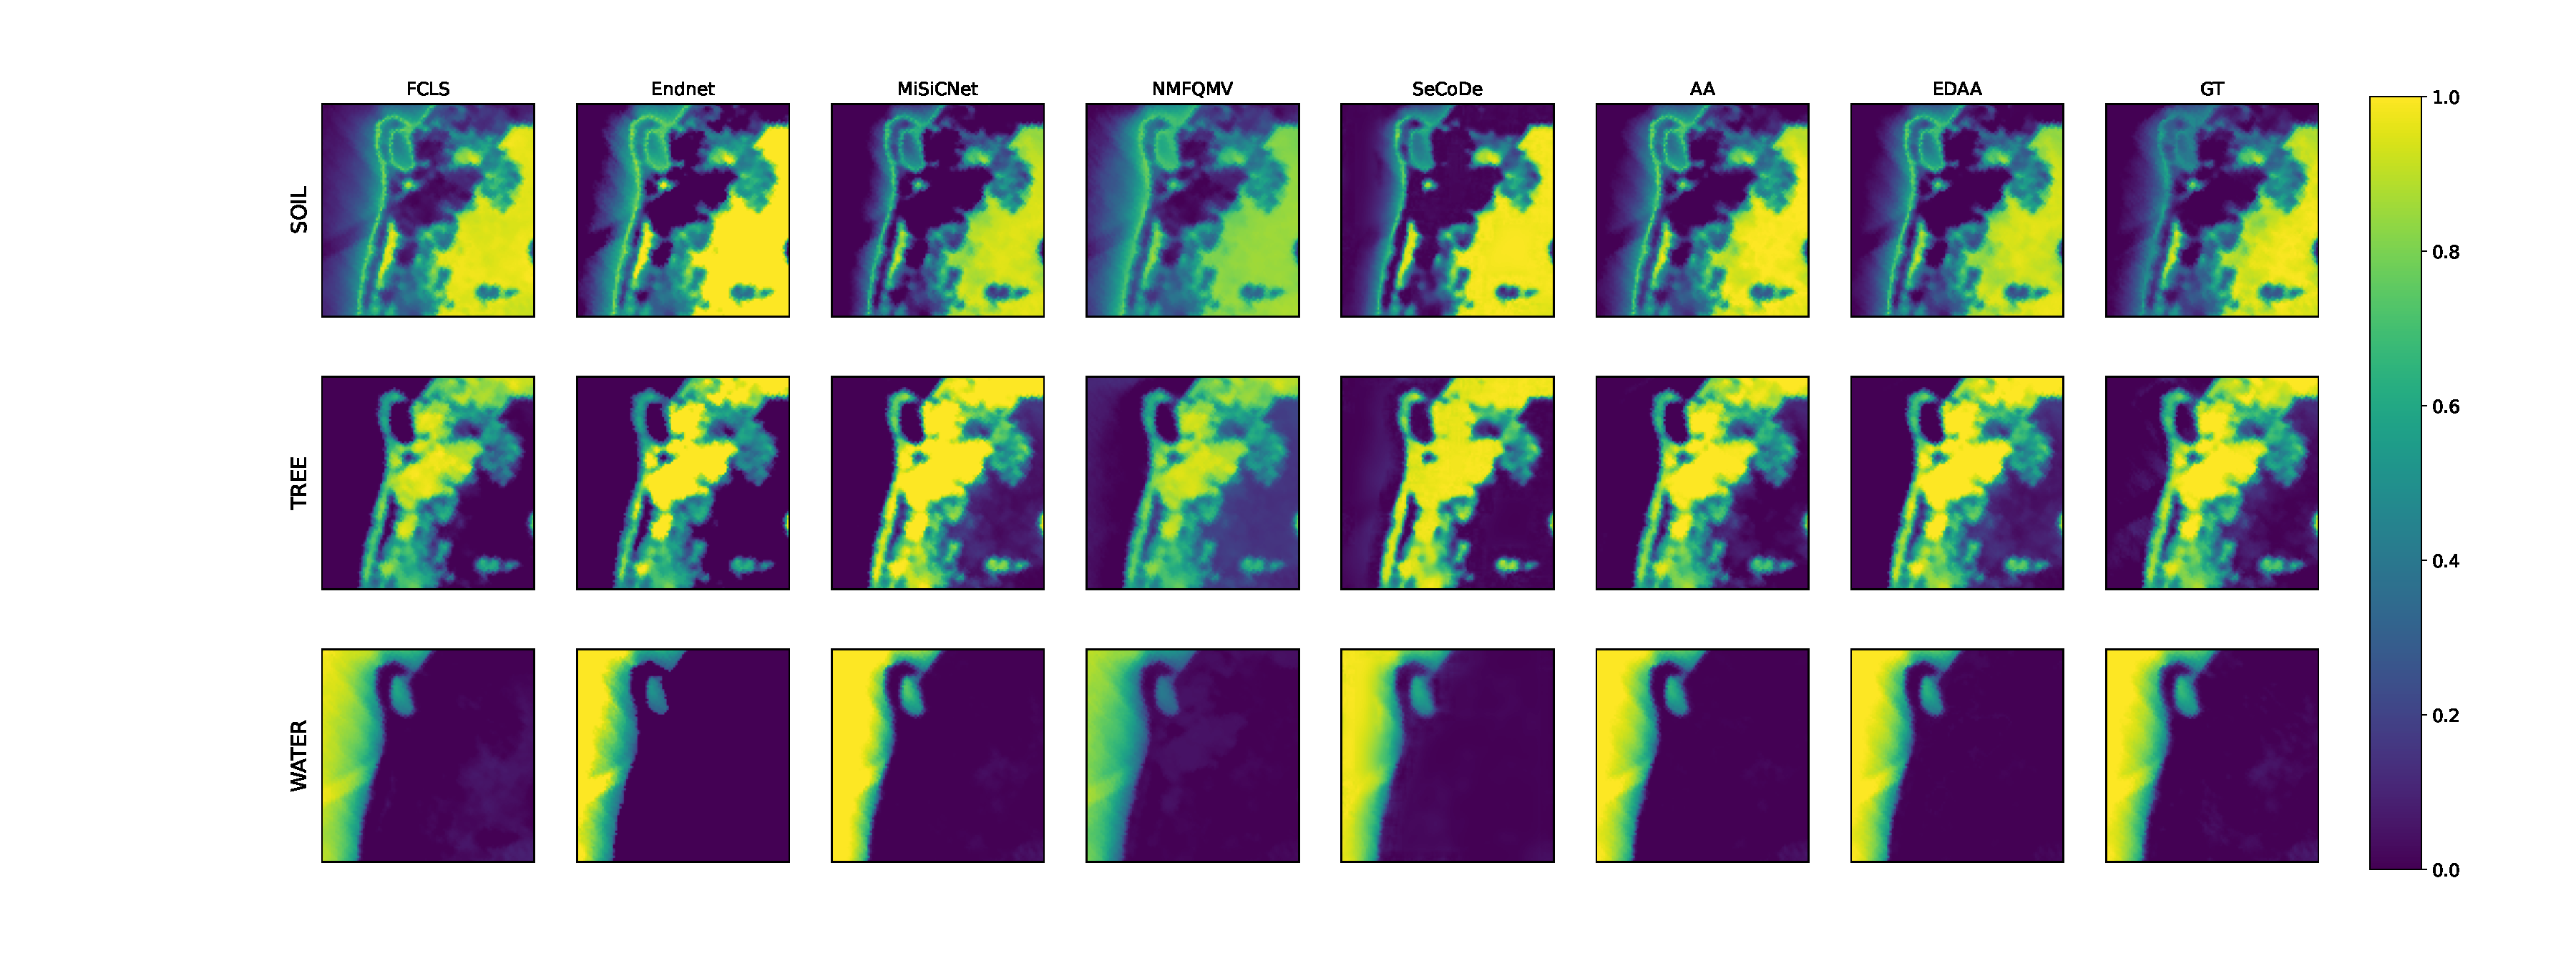
\includegraphics[width=\textwidth]{fichiers_latex/Chap2/figs/SamsonA-final.pdf}}
  \caption{\rev{Estimated endmembers (a) and abundances (b) on the Samson dataset. Ground truth abundances are displayed on the right-most column.}}
  \label{fig:Samson}
\end{figure}


\begin{figure}[h]
  \centering
  \subfloat[]{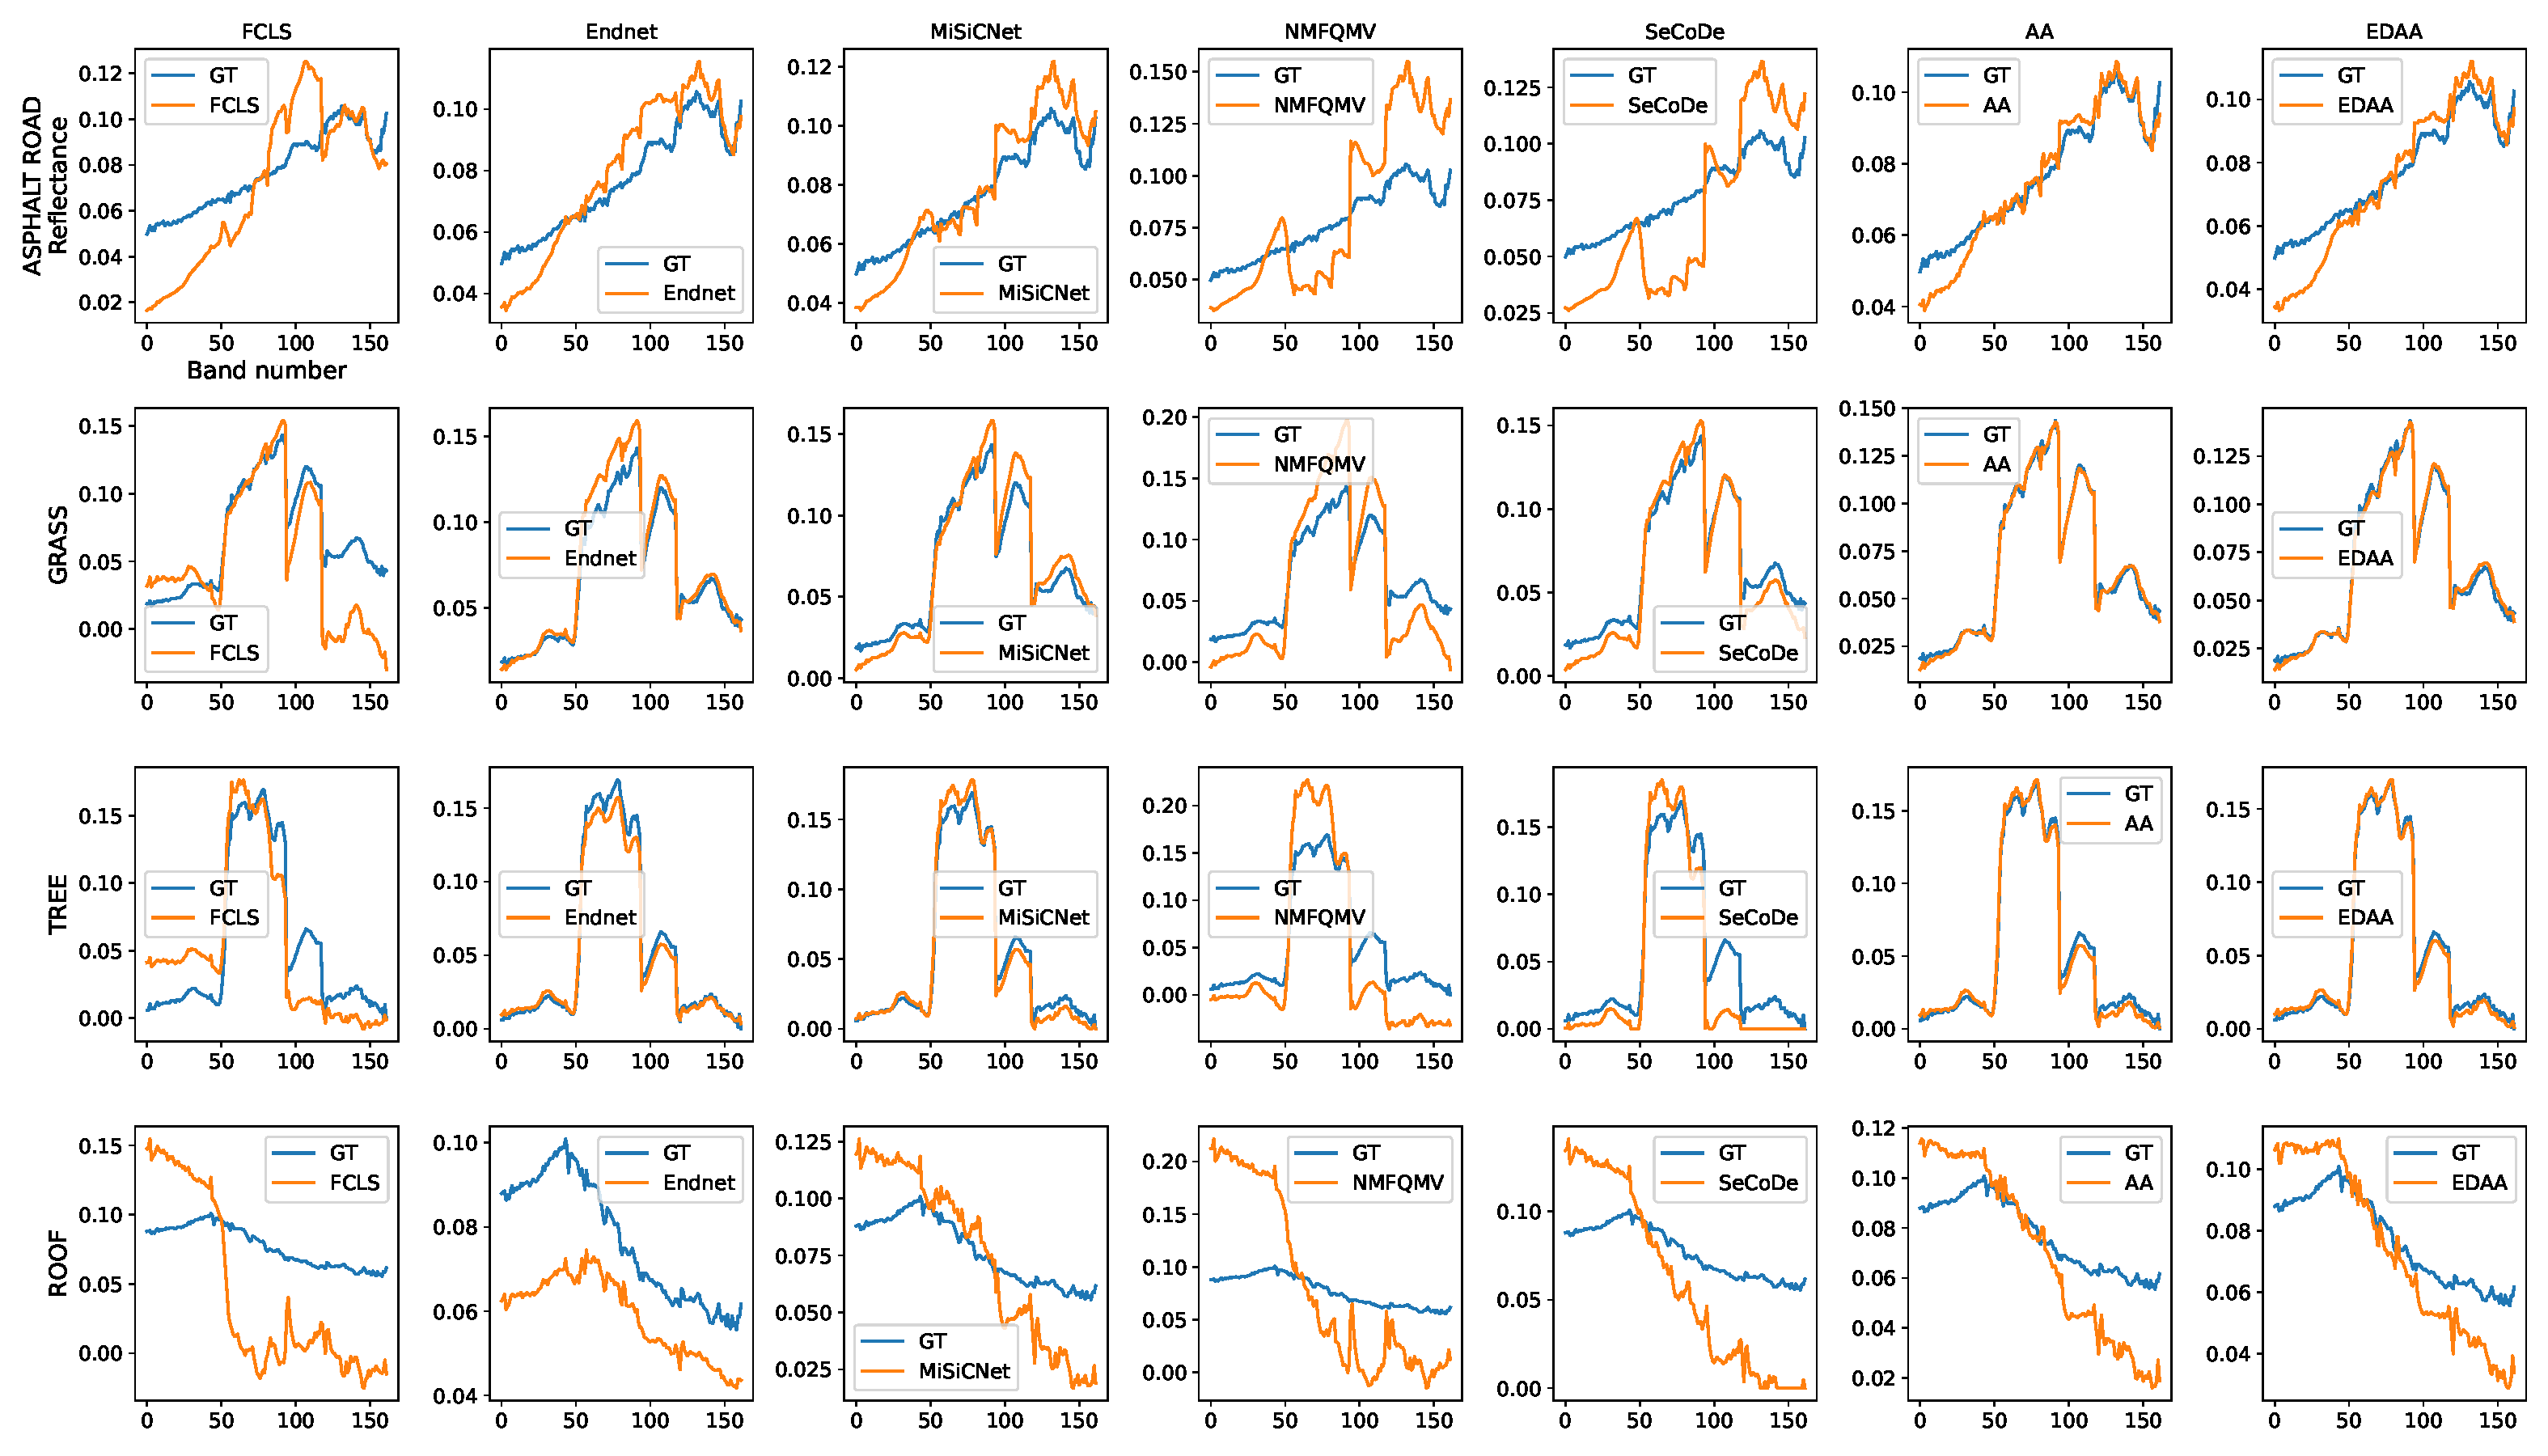
\includegraphics[width=\textwidth]{fichiers_latex/Chap2/figs/Urban4E-final.pdf}}
  \hfil
  \subfloat[]{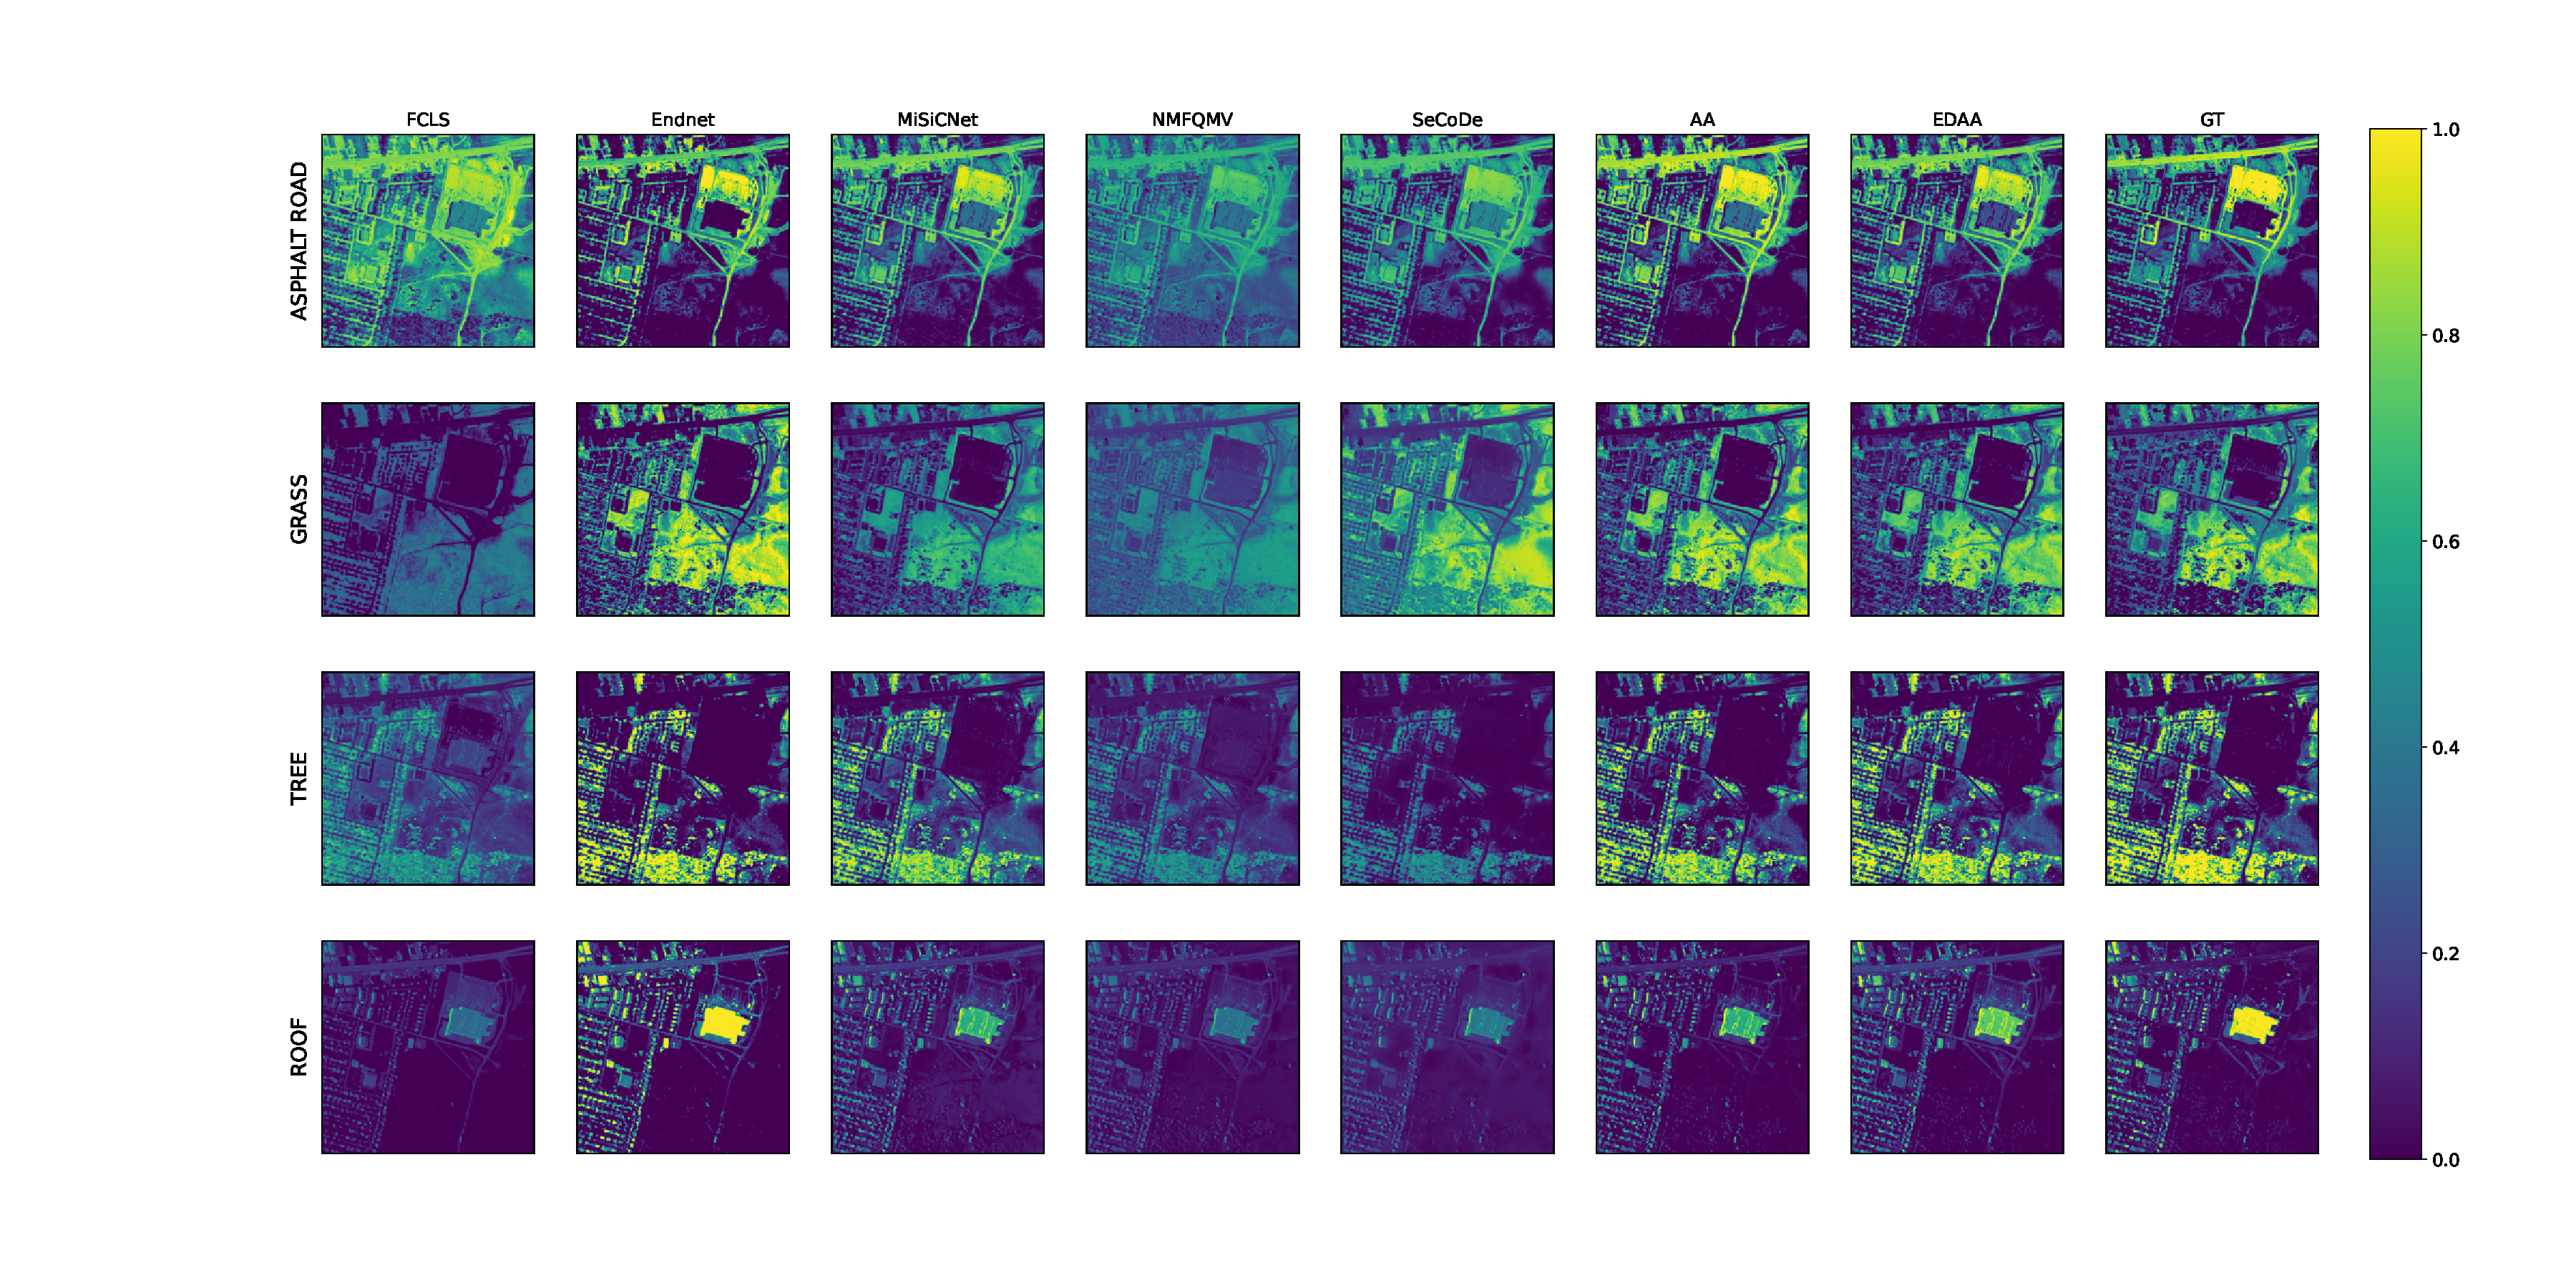
\includegraphics[width=\textwidth]{fichiers_latex/Chap2/figs/Urban4A-final.pdf}}
  \caption{\rev{Estimated endmembers (a) and abundances (b) on the Urban4 dataset. Ground truth abundances are displayed on the right-most column.}}
  \label{fig:Urban4}
\end{figure}

\begin{figure}[h]
  \centering
  \subfloat[]{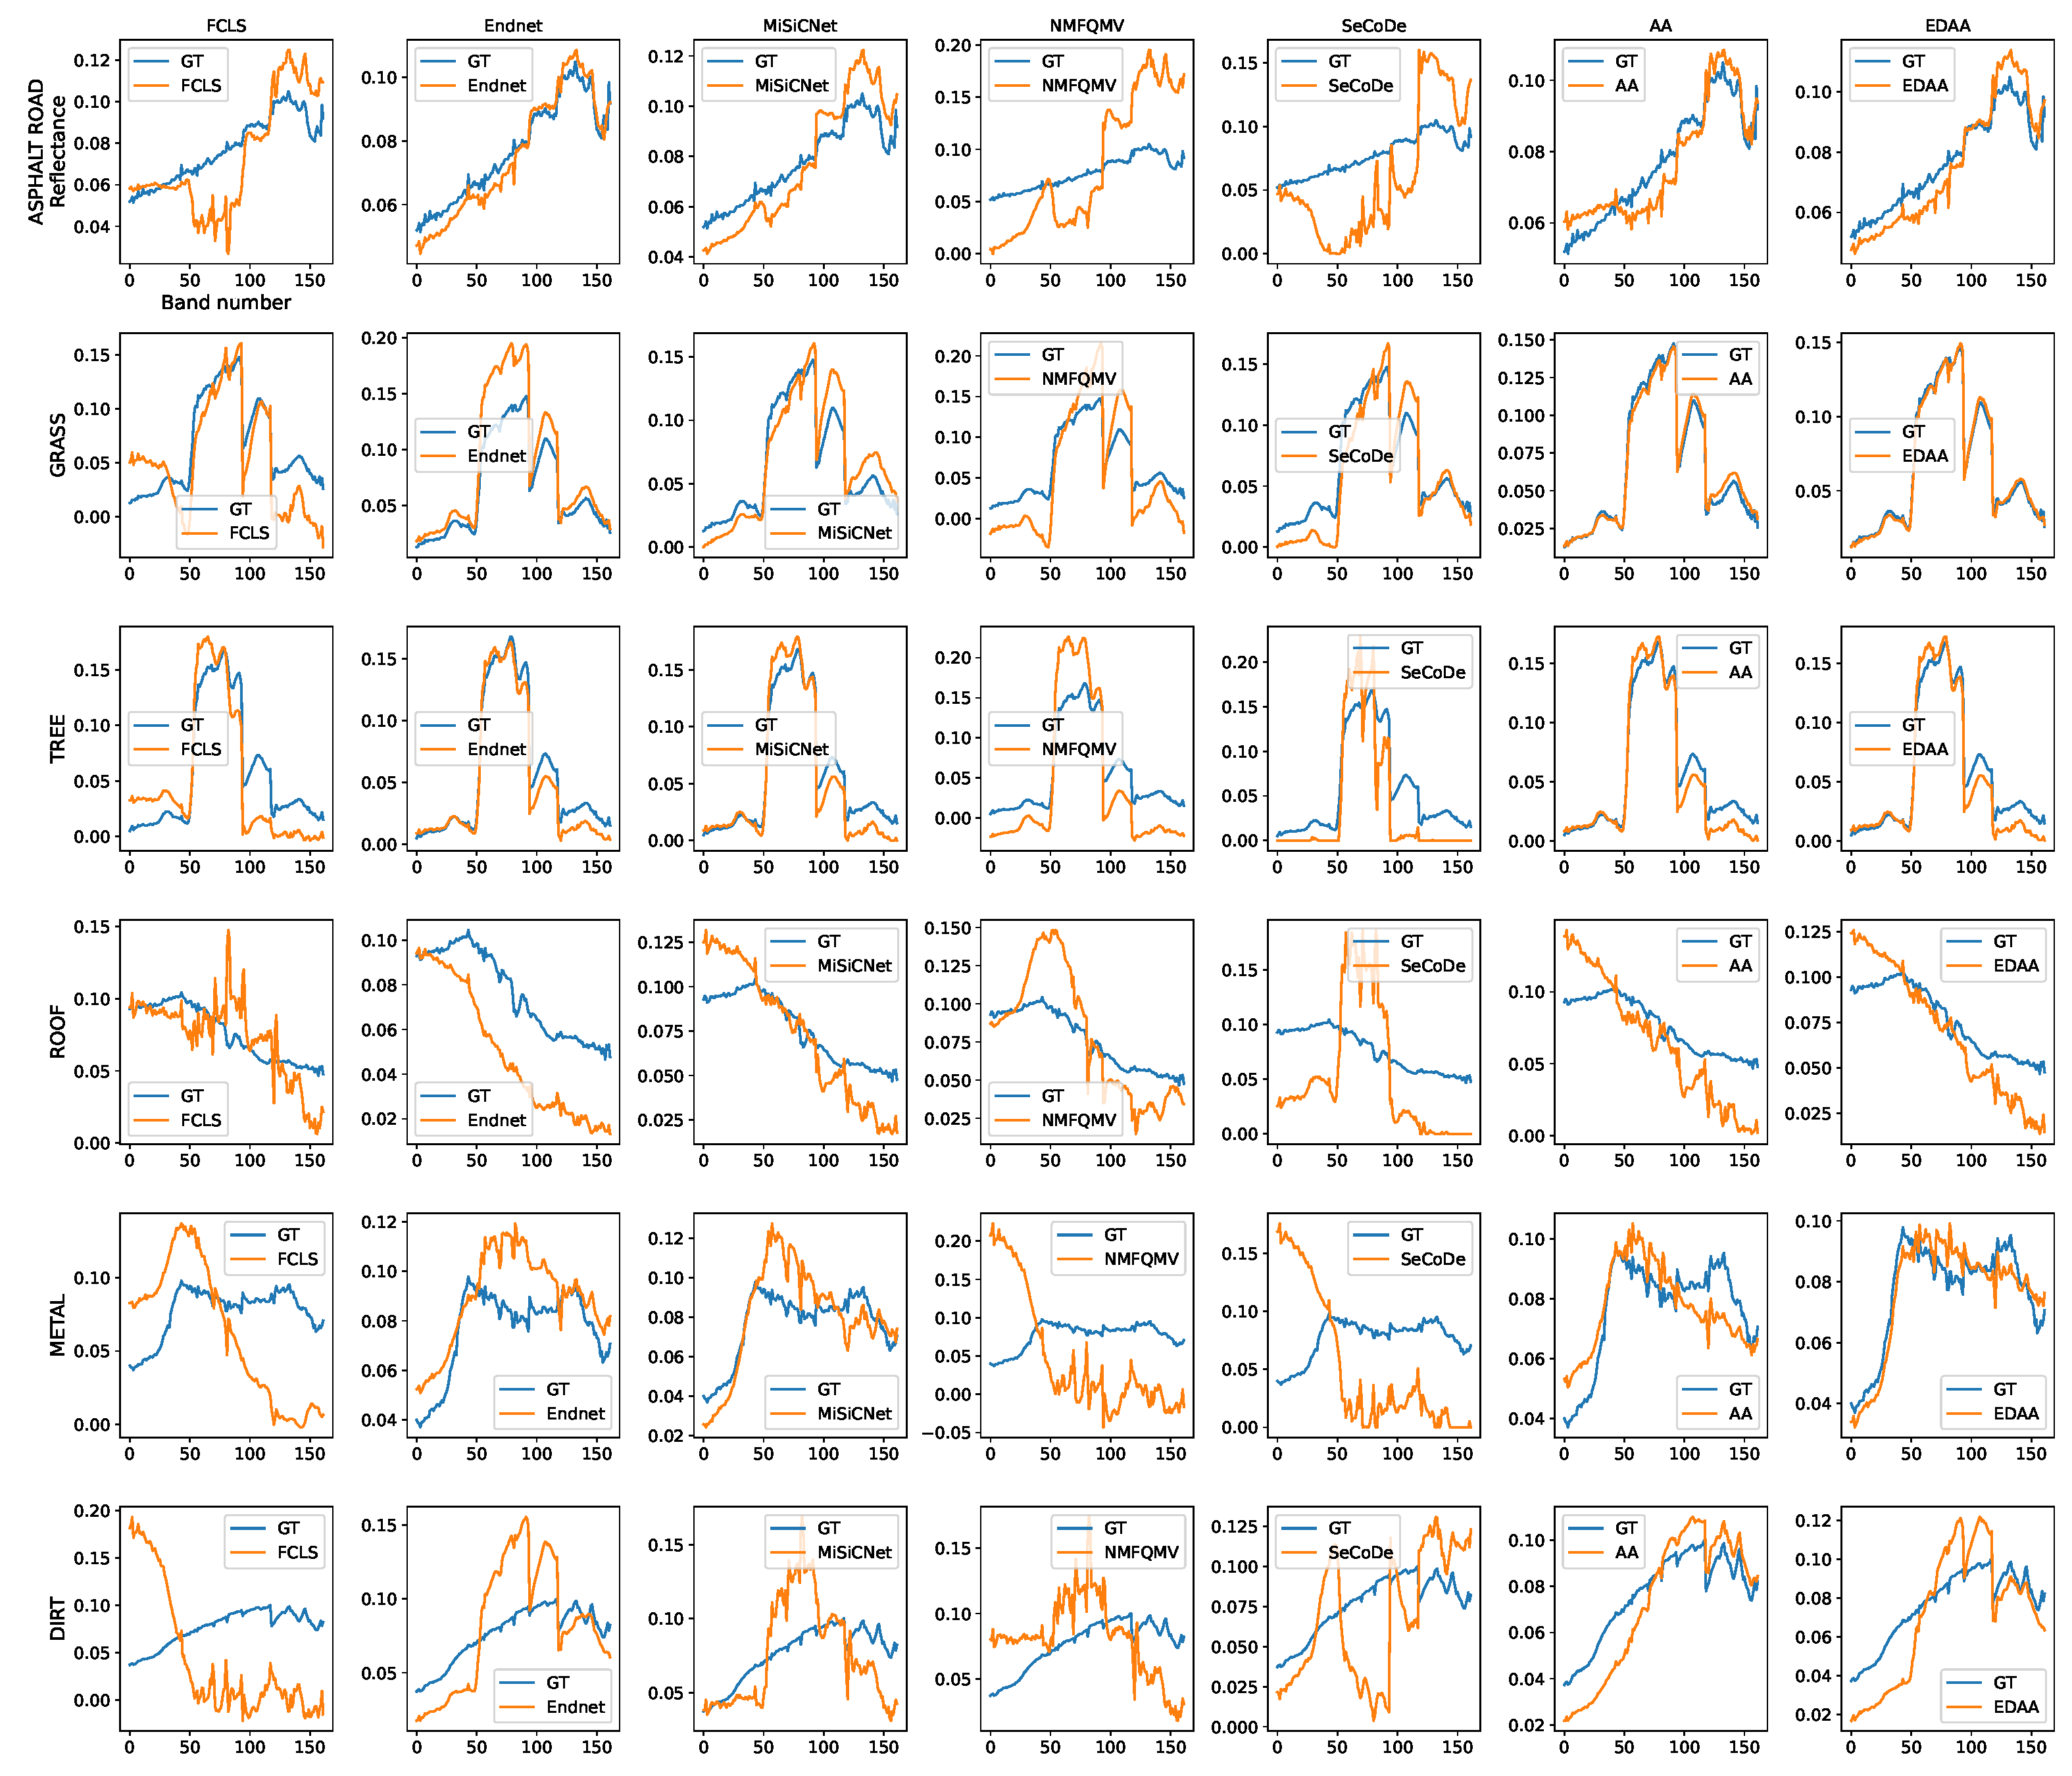
\includegraphics[width=0.66\textwidth]{fichiers_latex/Chap2/figs/Urban6E-final.pdf}}
  \hfil
  \subfloat[]{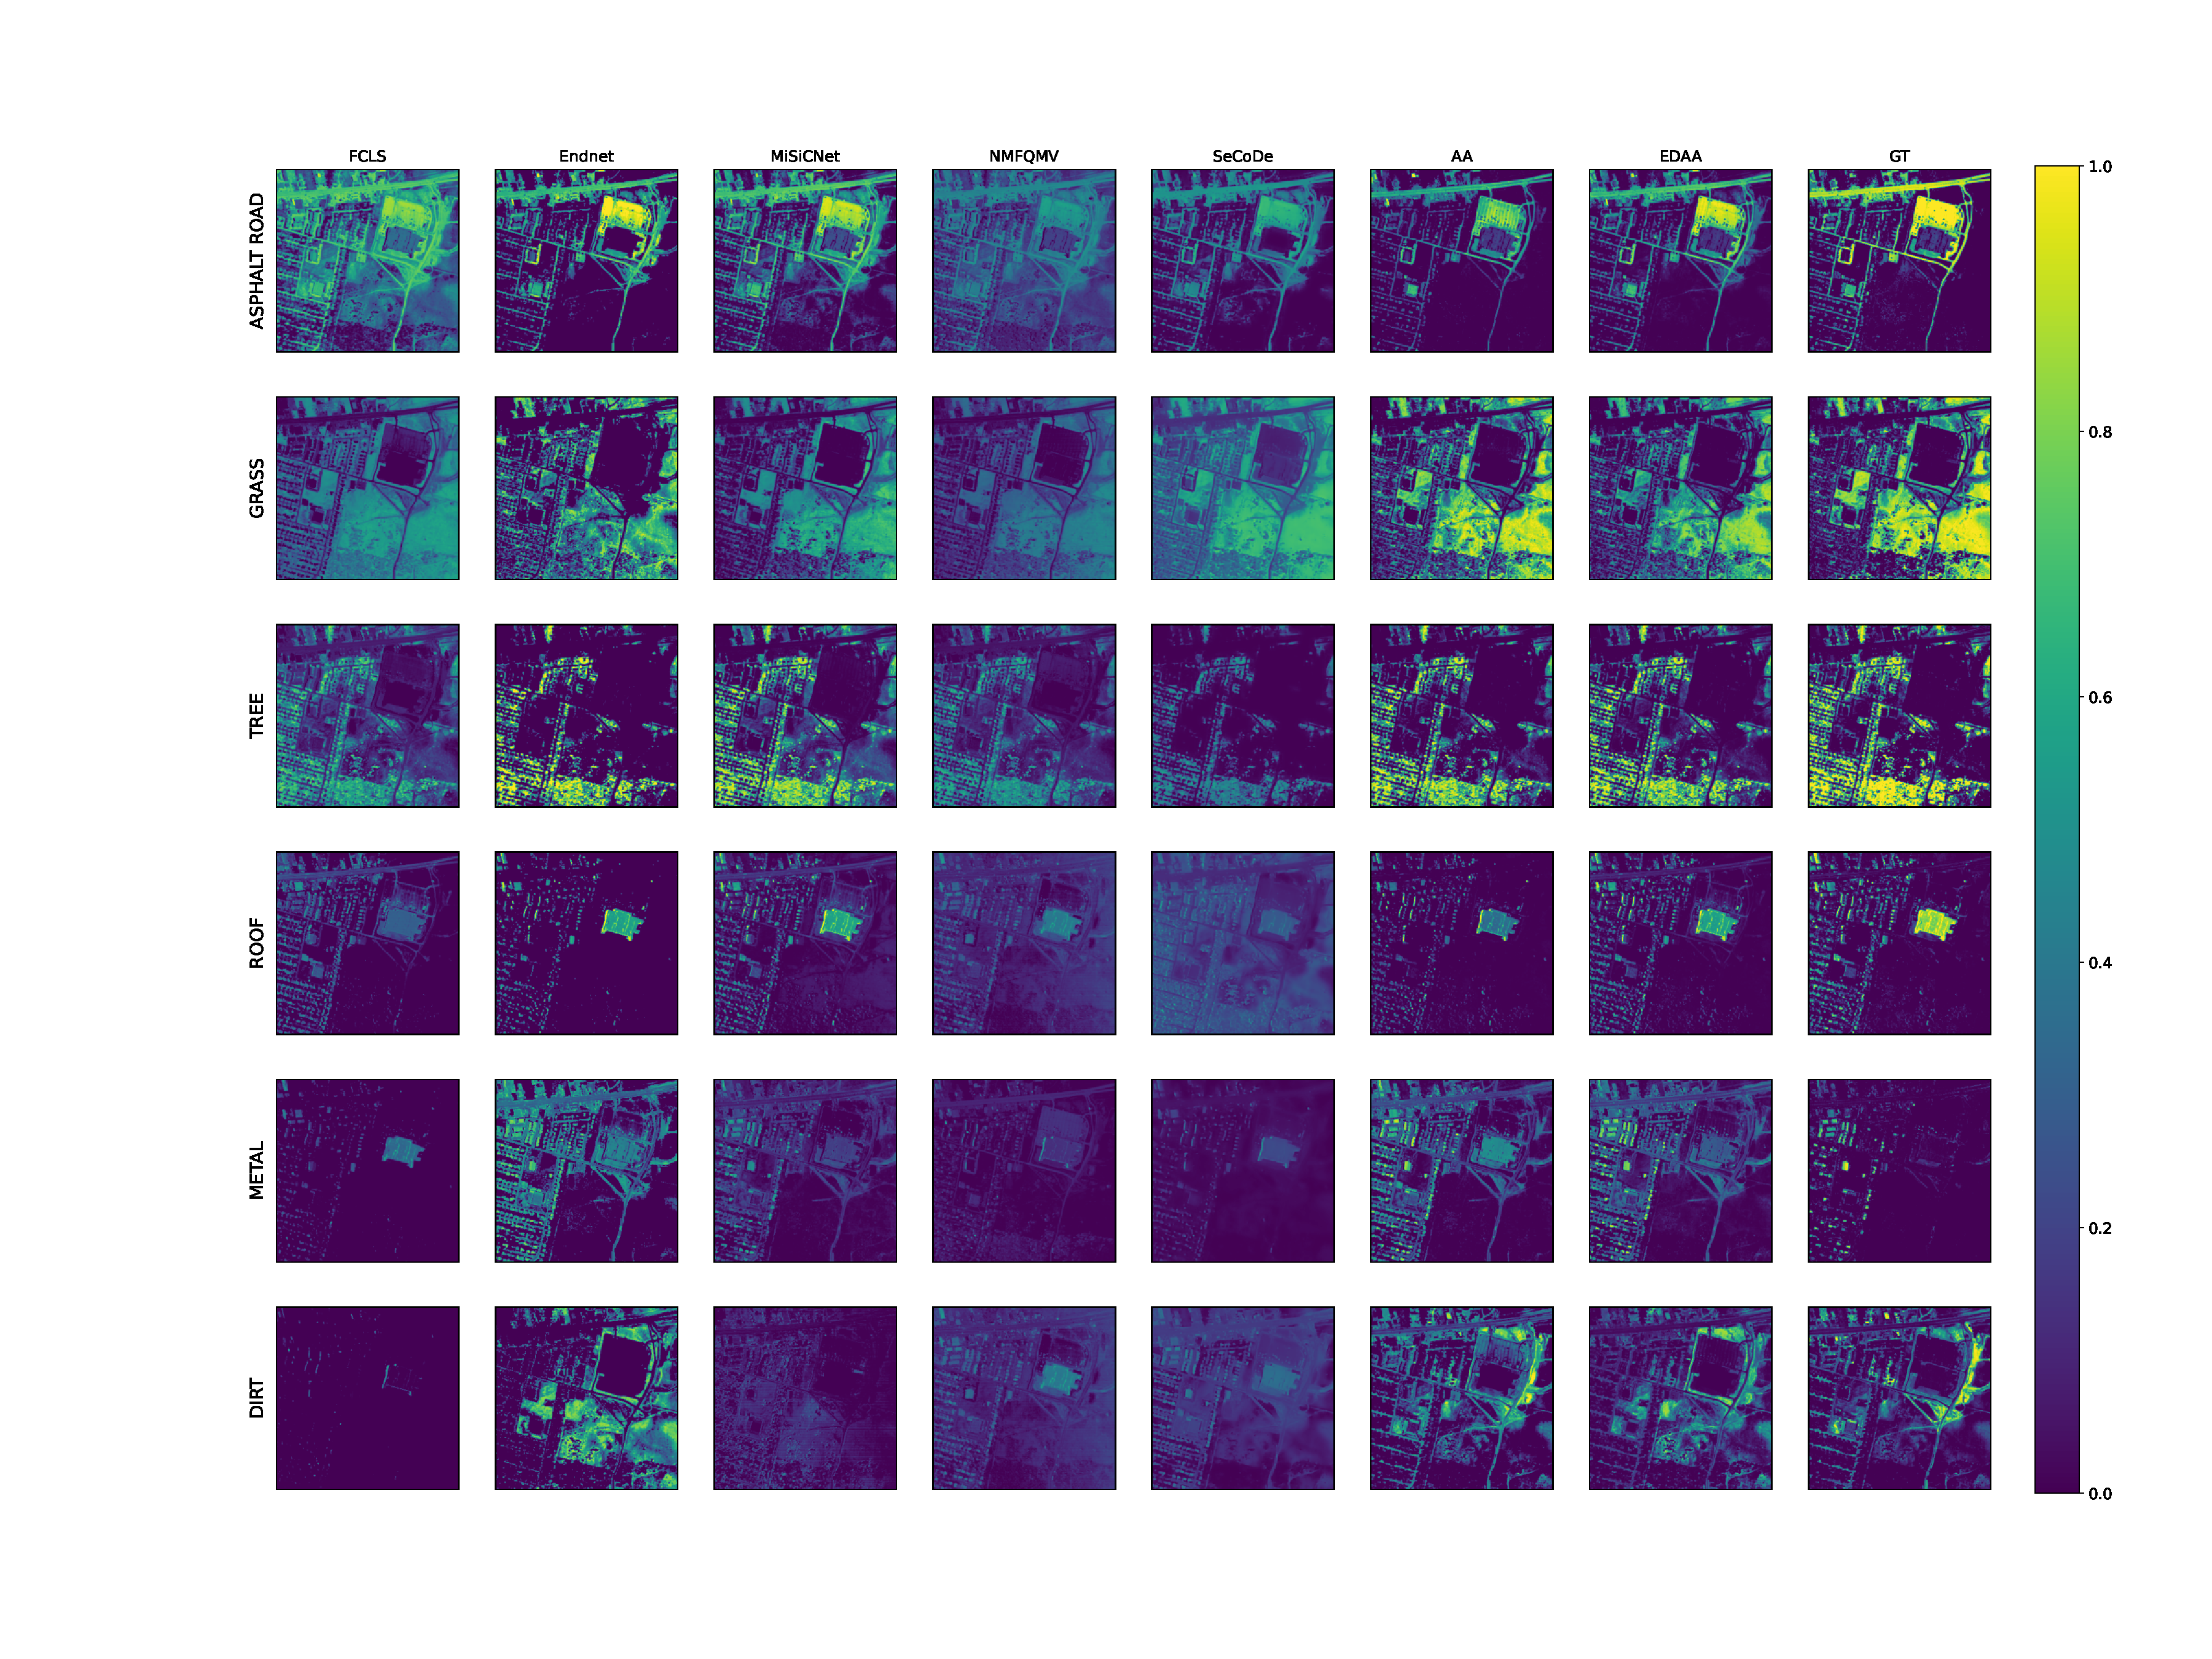
\includegraphics[width=\textwidth]{fichiers_latex/Chap2/figs/Urban6A-final.pdf}}
  \caption{\rev{Estimated endmembers (a) and abundances (b) on the Urban6 dataset.  Ground truth abundances are displayed on the right-most column.}}
  \label{fig:Urban6}
\end{figure}

\paragraph{Cuprite dataset}

\revision{
In order to evaluate the performance of the selected methods, we provide qualitative results on a 191 $\times$ 250 pixels subset of the Cuprite dataset, which is only accompanied by a geological map of the main materials present in the scene (see Fig.\ref{Real dataset}(a)). Recovering the spectral signatures of interest in this dataset is a challenging task due to the similarity of their spectral signatures and the presence of significant spectral variability. All methods were asked to output abundance maps for $r=5$ unknown endmembers. As shown in Fig.\ref{Real dataset}(b), all methods successfully recovered the three dominant materials of interest, namely Chalcedony, Alunite, and Kaolinite. However, we observed that MiSiCNet, AA, and EDAA produced sharper abundance maps than FCLS and NMFQMV. It is worth noting that we could not provide results for Endnet due to its outdated code base. Moreover, we had to increase the number of outer iterations for EDAA to 1000 to obtain meaningful results, while AA iterations could be kept at 100. Finally, we found that the $\ell_1$ fitting criterion was not satisfactory and had to be replaced with $\ell_2$ for this particular dataset.}

\begin{figure} [h]
\centering
\begin{tabular}{cc} 
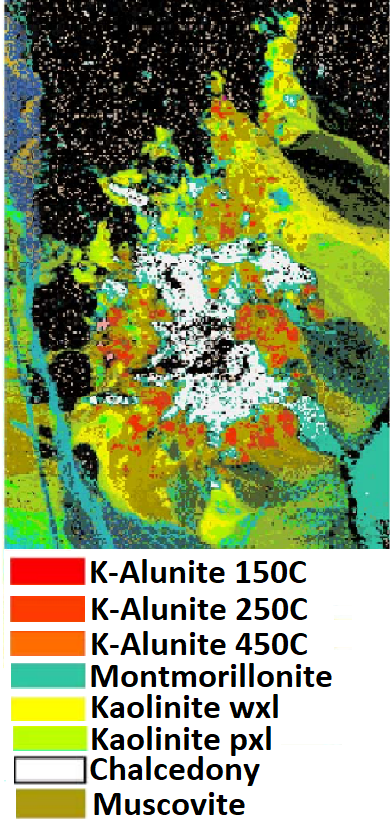
\includegraphics[width=.20\textwidth]{fichiers_latex/Chap2/figs/GRMap_Cup.png}&
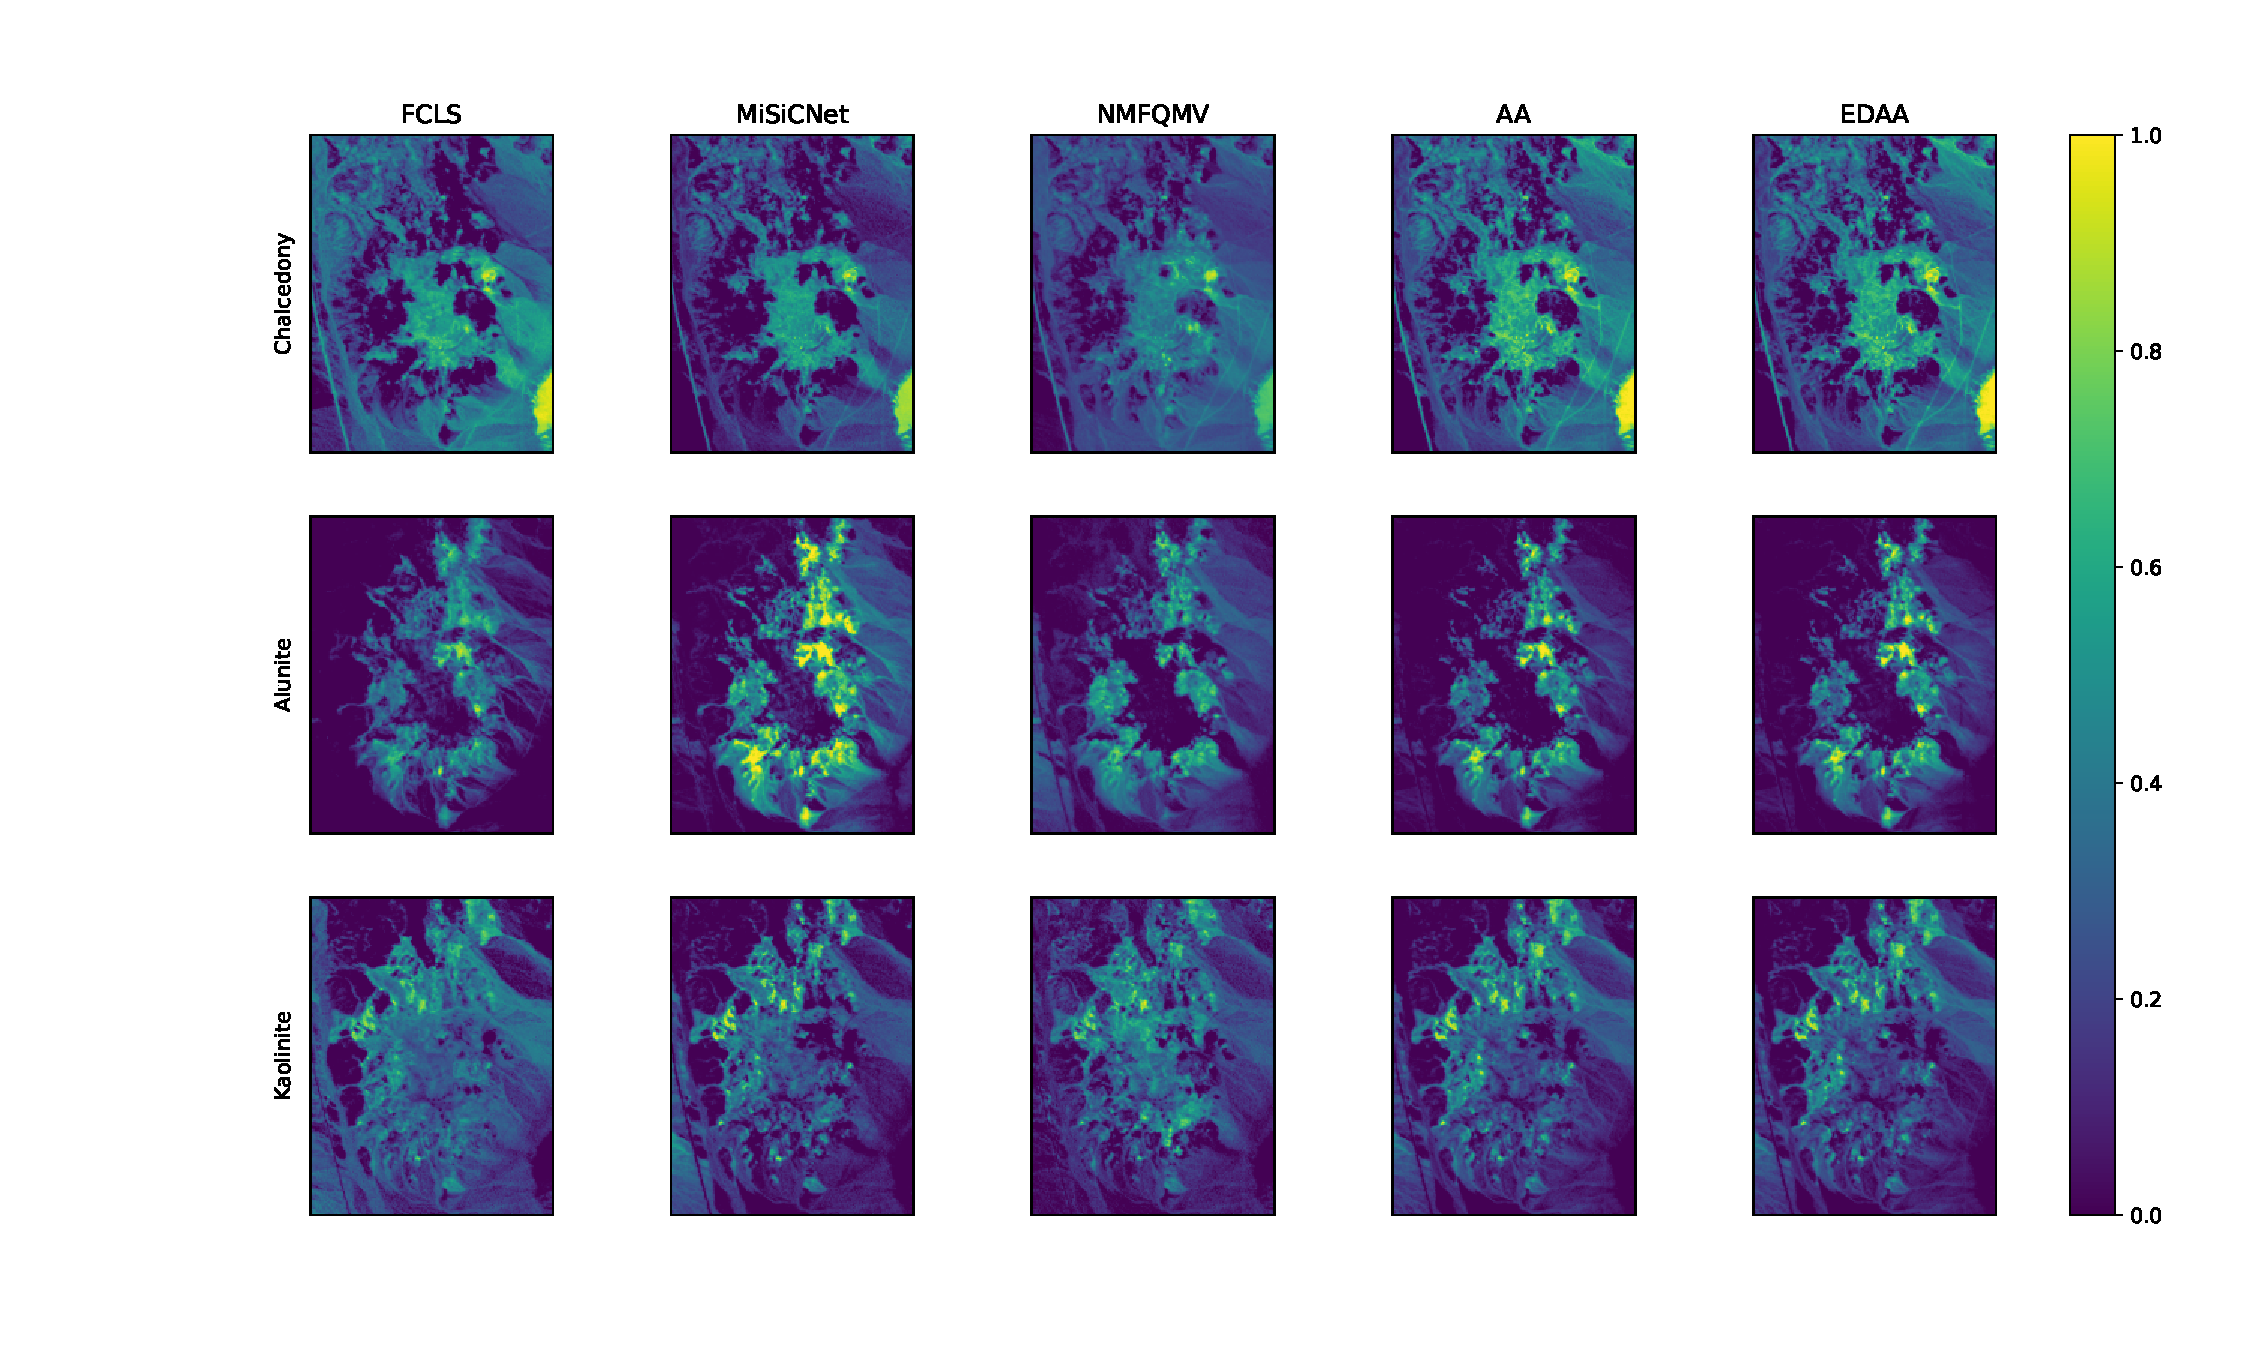
\includegraphics[width=.70\textwidth]{fichiers_latex/Chap2/figs/Cuprite_A.pdf}\\
 (a) Geological Map & (b) Estimated abundance maps
 \end{tabular} %\end{center} 
\caption{
\revision{Abundance maps of three dominant minerals estimated using different blind unmixing techniques applied to the Cuprite dataset.}
}
\label{Real dataset}
\end{figure}


\paragraph{Ablation study}

We report the detailed results obtained in the ablation study.
For each dataset, the overall abundances RMSE and SAD are computed for all configurations.
Table \ref{table:alg2} underlines the importance of the number of runs
$M$ in the model selection procedure.
Table \ref{table:alg1_decrease} studies the sensitivity of the outer iterations $T$ in EDAA when we decrease the computational budget.
Finally, table \ref{table:alg1_constant} studies the sensitivity of the inner and outer
iterations $K_1$, $K_2$ and $T$ in EDAA given a fixed computational budget.

\begin{table}[h]
\centering
  \captionof{table}{Sensitivity to the number of outer iterations $T$ of Algorithm
    EDAA with $K_1=K_2=5$. The abundances RMSE and SAD metrics are computed globally. The best results are in bold and the second best are underlined.}
    \begin{tabular}{c | c | c c c}
  \toprule
  & & $T=100$  & $T=75$ & $T=50$ \\
  \hline
  \multirow{2}{*}{Samson}
  & RMSE & \underline{4.24} & 4.34 & \textbf{3.97} \\
  & SAD &  \underline{1.64} & 1.69 & \textbf{1.46} \\
  \hline
  \multirow{2}{*}{Jasper Ridge}
  & RMSE &  6.85 & \textbf{5.90} & \underline{6.44} \\
  & SAD &  3.22 & \textbf{3.06} & \underline{3.19} \\
  \hline
  \multirow{2}{*}{Urban4}
  & RMSE & \underline{7.51} & \textbf{7.46} & 7.72 \\
  & SAD & 5.87 & \underline{5.01} & \textbf{4.67} \\
  \hline
  \multirow{2}{*}{Urban6}
  & RMSE & \textbf{13.52} & \underline{13.54} & 13.99 \\
  & SAD &  7.95 & \textbf{7.85} & \underline{7.93} \\
  \hline
  \multirow{2}{*}{APEX}
  & RMSE & 14.66 & \underline{14.38} & \textbf{14.12} \\
  & SAD & \textbf{6.29} & \underline{6.58} & 6.99 \\
  \hline
  \multirow{2}{*}{WDC}
  & RMSE & \textbf{20.47} & \underline{22.81} & 22.89 \\
  & SAD & \textbf{12.33} & 16.97 & \underline{16.87} \\

  \bottomrule
\end{tabular}
  \label{table:alg1_decrease}
\end{table}

\begin{table}[h]
  \captionof{table}{Sensitivity to the number of runs $M$ of the model selection
    procedure with $K_1=K_2=5$ and $T=100$. The abundances RMSE and SAD metrics are computed globally. The best results are in bold and the second best are underlined.}
    \begin{tabular}{c | c | c c c c}
  \toprule
  & & $M=10$  & $M=20$ & $M=50$ & $M=100$ \\
  \hline
  \multirow{2}{*}{Samson}
  & RMSE & 5.05 & \textbf{3.90} & \underline{4.24} & \underline{4.24} \\
  & SAD & 1.94 & \textbf{1.43} & \underline{1.64} &\underline{1.64} \\
  \hline
  \multirow{2}{*}{Jasper Ridge}
  & RMSE & 10.27 & 10.27 & \textbf{6.85} & \textbf{6.85} \\
  & SAD & 3.73 & 3.73 & \textbf{3.22} & \textbf{3.22} \\
  \hline
  \multirow{2}{*}{Urban4}
  & RMSE & 8.17 & 8.06 & \underline{7.75} & \textbf{7.51} \\
  & SAD & 5.43 & \underline{5.41} & \textbf{5.36} & 5.87 \\
  \hline
  \multirow{2}{*}{Urban6}
  & RMSE & 16.50 & 16.50 & \underline{13.63} &\textbf{13.52} \\
  & SAD & 8.16 & 8.16 & \textbf{7.92} & \underline{7.95} \\
  \hline
  \multirow{2}{*}{APEX}
  & RMSE & 23.84 & 24.17 & \underline{14.94} & \textbf{14.66} \\
  & SAD & 12.57 & 12.88 & \textbf{6.06} &\underline{6.29} \\
  \hline
  \multirow{2}{*}{WDC}
  & RMSE & 24.39 & 24.39 & \textbf{20.46} &\underline{20.47} \\
  & SAD & \textbf{11.52} & \textbf{11.52} & 12.40 & 12.33 \\
  \bottomrule
\end{tabular}
  \label{table:alg2}
\end{table}

\begin{table}[h]
  \captionof{table}{Sensitivity to hyperparameters of EDAA
    for a constant number of updates (1000). The abundances RMSE and SAD metrics are computed globally. The best results are in bold and the second best are underlined.}
  \begin{adjustbox}{width=\textwidth}
    \begin{tabular}{c | c | c c c c c}
  \toprule
  & & $K_1=K_2=1$, $T=500$ & $K_1=K_2=5$, $T=100$  & $K_1=K_2=10$, $T=50$ & $K_1=K_2=20$, $T=25$ & $K_1=K_2=50$, $T=10$ \\
  \hline
  \multirow{2}{*}{Samson}
  & RMSE & 4.42 & \underline{4.24} & \textbf{4.15} & 4.48 & 4.34 \\
  & SAD & 1.65 & \underline{1.64} & \textbf{1.61} & 1.78 & 1.68 \\
  \hline
  \multirow{2}{*}{Jasper Ridge}
  & RMSE & \textbf{6.70} & \underline{6.85} & 7.80 & 7.59 & 8.79 \\
  & SAD & 3.48 & \underline{3.22} & 4.28 & \textbf{3.12} & 4.79 \\
  \hline
  \multirow{2}{*}{Urban4}
  & RMSE & \textbf{7.40} & 7.51 & \underline{7.43} & 7.90 & 9.49 \\
  & SAD & 5.72 & 5.87 & \underline{5.53} & 6.05 & \textbf{5.46} \\
  \hline
  \multirow{2}{*}{Urban6}
  & RMSE & 17.92 & 13.52 & \textbf{12.35} & \underline{12.71} & 17.92 \\
  & SAD & 11.71 & \textbf{7.95} & 8.74 & \underline{8.52} & 8.79 \\
  \hline
  \multirow{2}{*}{APEX}
  & RMSE & 14.25 & 14.66 & \underline{14.20} & \textbf{14.15} & 16.46\\
  & SAD & 8.17 & \underline{6.29} & 7.73 & 8.06 & \textbf{5.26} \\
  \hline
  \multirow{2}{*}{WDC}
  & RMSE & 22.91 & \textbf{20.47} & 22.16 & \underline{20.92} & 21.20 \\
  & SAD & \underline{12.59} & \textbf{12.33} & 16.05 & 13.46 & 13.51 \\

  \bottomrule
\end{tabular}
  \end{adjustbox}
  \label{table:alg1_constant}
\end{table}



